
\documentclass[a4paper, 12pt]{report}

\usepackage[spanish,es-tabla]{babel}

\makeatletter

%!TEX root = rdegiovanni-phd-tesis.tex
\usepackage[parts]{classicthesis} 

%\usepackage[left=1.5in,right=1.5in,top=1.5in,bottom=1.5in]{geometry} %configure margins
%\usepackage[left=3.65cm,right=3.65cm,bindingoffset=0.5cm]{geometry} %raul config

%%Options: Sonny, Lenny, Glenn, Conny, Rejne, Bjarne, Bjornstrup
%\usepackage[Bjarne]{fncychap}

\usepackage[T1]{fontenc}
% manual chapter style
%\newcommand\mychapterNumber{\normalfont\fontfamily{pplj}\fontsize{35}{36}\selectfont}
%\titleformat{\chapter}[block]%
%  {\vspace*{-2cm}}{\color{halfgray}\mychapterNumber\thechapter}{1em}
%  {\raggedright\spacedallcaps}[\normalsize\vspace*{.8\baselineskip}\color{halfgray}{\titlerule[2pt]}]%


% General useful packages
\usepackage[spanish, es-tabla, es-noquoting]{babel}
\usepackage{amsmath,amsthm,amssymb,verbatim}
\usepackage{graphicx}
\usepackage{caption}
\usepackage{subcaption}
\usepackage{alltt}
\renewcommand{\ttdefault}{txtt}
\usepackage{mathrsfs}
\usepackage{stmaryrd}
%\usepackage[hidelinks]{hyperref}
\usepackage{enumitem}
\usepackage{proof}
\usepackage{lscape}
\usepackage{booktabs}
\usepackage{tikz}
\usetikzlibrary{matrix,chains,positioning,calc,shadows,fit,arrows, shapes, shapes.geometric, petri} 
\usetikzlibrary{decorations.text, decorations.markings,decorations.pathreplacing} %calc,decorations.pathmorphing}
%\usetikzlibrary{shapes,fit,arrows,calc,positioning, decorations.pathreplacing}

%citations
\usepackage[hyperpageref]{backref}
\usepackage{cite}
\renewcommand\citepunct{; }

%paragraph space
\setlength{\parskip}{.2cm}%\baselineskip}

% import tikz styles
%\input{LTS-style}

% listings
\usepackage{listings}
\definecolor{lightgray}{gray}{.60}
\definecolor{Lightgray}{gray}{.98}
\definecolor{bordegray}{gray}{.70}
\definecolor{gray}{gray}{.3}

% Hyperreferences
\hypersetup{%
    %draft,	% = no hyperlinking at all (useful in b/w printouts)
    colorlinks=true, linktocpage=true, pdfstartpage=3, pdfstartview=FitV,%
    % uncomment the following line if you want to have black links (e.g., for printing)
    %colorlinks=false, linktocpage=false, pdfborder={0 0 0}, pdfstartpage=3, pdfstartview=FitV,% 
    breaklinks=true, pdfpagemode=UseNone, pageanchor=true, pdfpagemode=UseOutlines,%
    plainpages=false, bookmarksnumbered, bookmarksopen=true, bookmarksopenlevel=1,%
    hypertexnames=true, pdfhighlight=/O,%nesting=true,%frenchlinks,%
    urlcolor=webbrown, linkcolor=RoyalBlue, citecolor=gray!20!RoyalBlue %webgreen, %pagecolor=RoyalBlue,%
    %urlcolor=Black, linkcolor=Black, citecolor=Black, %pagecolor=Black,%
}


% References
\usepackage[spanish]{cleveref}
\crefname{figure}{Figura}{Figuras}
\crefname{table}{Tabla}{Tablas}
\crefname{chapter}{Cap\'itulo}{Cap\'itulos}
\crefname{section}{Secci\'on}{Secciones}
\crefname{subsection}{Subsecci\'on}{Subsecciones}
\crefname{definition}{Definici\'on}{Definiciones}
\crefname{theorem}{Teorema}{Teoremas}
\crefname{lemma}{Lema}{Lemas}
\crefname{algorithm}{Algoritmo}{Algoritmos}
%\renewcommand{\figureautorefname}{Figura}%
%\renewcommand{\figureautorefname}{Figura}%
%\renewcommand{\tableautorefname}{Tabla}%
%\renewcommand{\partautorefname}{Parte}%
%\renewcommand{\chapterautorefname}{Cap\'itulo}%
%\renewcommand{\sectionautorefname}{Secci\'on}%
%\renewcommand{\subsectionautorefname}{Secci\'on}%
%\renewcommand{\subsubsectionautorefname}{Secci\'on}% 	
%\renewcommand{\listtablename}{\'Indice de Tablas}
% ********************************************************************
% Using different fonts
% ********************************************************************
%\usepackage[oldstylenums]{kpfonts} % oldstyle notextcomp
%\usepackage[osf]{libertine}
%\usepackage{hfoldsty} % Computer Modern with osf
%\usepackage[light,condensed,math]{iwona}
%\renewcommand{\sfdefault}{iwona}
\usepackage{lmodern} % <-- no osf support :-(
%\usepackage[urw-garamond]{mathdesign} <-- no osf support :-(
% ****************************************************************************************************

% Personal data and user ad-hoc commands
\newcommand{\ingles}[1]{#1}
\newcommand{\lenguaje}[1]{{\sc#1}}
\newcommand{\herramienta}[1]{\textsf{#1}}
\newcommand{\codigo}[1]{\texttt{#1}}
\newcommand{\FSPcode}[1]{\colorbox{gray!10}{\textcolor{black}{\tt #1}}}
\newcommand{\ALVcode}[1]{\colorbox{gray!10}{\textcolor{black!80}{\tt #1}}}

% Teoremas, Lemas, Definiciones y Ejemplos
\newtheorem{theorem}{Teorema}[chapter]
\newtheorem{lemma}[theorem]{Lema}
\newtheorem{definition}{Definici\'on}[chapter]
\newtheorem{example}{Ejemplo}[chapter]


\newcommand{\tituloES}{Expresiones de navegaci\'on, el mutante perdido.}

\newcommand{\HRule}{\rule{\linewidth}{0.5mm}}

%%% 
\newcommand{\SAT}[1]{\models_{\scriptscriptstyle{#1}}}
\newcommand{\LTSproc}[1]{\textbf{\texttt{#1}}}
\newcommand{\Fluent}[1]{\textit{#1}}

\newcommand{\GoalDef}[1]{\fbox{\parbox{\textwidth}{#1}}}

%% Algoritmos
\usepackage[chapter]{algorithm}
% \usepackage[noend]{algpseudocode}
% New definitions
% \algnewcommand\algorithmicswitch{\textbf{switch}}
% \algnewcommand\algorithmiccase{\textbf{case}}
% \algnewcommand\algorithmicassert{\texttt{assert}}
% \algnewcommand\Assert[1]{\State \algorithmicassert(#1)}%
% New "environments"
% \algdef{SE}[SWITCH]{Switch}{EndSwitch}[1]{\algorithmicswitch\ #1\ \algorithmicdo}{\algorithmicend\ \algorithmicswitch}%
% \algdef{SE}[CASE]{Case}{EndCase}[1]{\algorithmiccase\ #1}{\algorithmicend\ \algorithmiccase}%
% \algtext*{EndSwitch}%
% \algtext*{EndCase}%
% \newcommand{\Break}{\State \textbf{break} }
% \newcommand{\Continue}{\textbf{continue} }
%\algnewcommand{\LineComment}[1]{\State \algorithmicend\ right\) #1}
% \algnewcommand{\LineComment}[1]{\State {\small \(--\) #1}}
% \algnewcommand{\MyComment}[1]{{\small \(--\) #1}}
%\newcommand{\Let}{\State \textbf{let} }
% \algblockdefx{Let}{EndLet}[1]{\textbf{let} #1 \textbf{in}}{\textbf{endlet}}
% \algtext*{EndLet}%

\usepackage[utf8]{inputenc}

\usepackage[utf8]{inputenc}
\usepackage[spanish]{babel}

\usepackage{titletoc}
\usepackage{tikz}
\usetikzlibrary{shapes,arrows,positioning}
\renewcommand{\lstlistingname}{Figure}% Listing -> Figure

 % Add new own commands
\newcommand{\cacho}{\textcolor{red}}
\usepackage{colortbl}
\newcommand{\hightlight}{\rowcolor[gray]{.95}}

% Define el comando \cellcolorgray para aplicar sombreado a una celda
\newcommand{\cellcolorgray}{\cellcolor{gray!25}}%Indice
\renewcommand{\cftchapleader}{\cftdotfill{\cftdotsep}} % Agrega puntos para las secciones
\titlecontents{chapter}
  [0em]
  {\vspace{1em}\bfseries}
  {\thecontentslabel.\enspace}
  {}
  {\hfill\contentspage} % Mueve el número de página a la derecha
\titlecontents{section}
  [2em]
  {}
  {\thecontentslabel.\enspace}
  {}
  {\titlerule*[0.75em]{.}\contentspage} % Agrega líneas de puntos para las secciones
\titlecontents{subsection}
  [4.5em]
  {}
  {\thecontentslabel.\enspace}
  {}
  {\titlerule*[0.75em]{.}\contentspage} % Agrega líneas de puntos para las subsecciones

%Formato para chapter

\titleformat{\chapter}[display]{\normalfont\Huge\bfseries}{\chaptertitlename\ \thechapter.}{0.42em}{}
\titleformat{\section}{\bfseries}{\thesection}{1em}{}
% chktex-file 1

\titleformat{\subsection}{\bfseries}{\thesubsection}{1em}{}

\titlespacing{\chapter}{0pt}{0pt}{4pt}
% Configuración del estilo de página
% \fancypagestyle{mypagestyle}{
%     \fancyhf{} % Limpiar encabezado y pie de página
%     \renewcommand{\headrulewidth}{0pt} % Eliminar la línea horizontal del encabezado
%     \fancyfoot[C]{\thepage} % Número de página alineado a la derecha en el pie de página
% }

% Aplicar el estilo de página a todo el documento
% \pagestyle{mypagestyle}

\usepackage{arydshln}

\babelhyphenation[spanish]{Node-Caching-Linked-List}
\definecolor{dkgreen}{rgb}{0,0.6,0}
\usepackage{listings}
\lstset{ %this is the stype
        captionpos=b,
        mathescape=true,
        texcl=false,
        frame=tb,
        language=Java,
        numbers=left,
      	aboveskip=0mm,
      	belowskip=0mm,
      	showstringspaces=false,
      	columns=flexible,
      	basicstyle={\scriptsize\ttfamily}, 
        keywordstyle=\color{blue}\bfseries,
        commentstyle=\color{dkgreen},
        morekeywords={,input, output, return, datatype, function, in, if, then, else, foreach, while, begin, end, inputs, outputs, procedure, for, do, done, fi, break, not, local, continue, and,} %add the keywords you want, or load a language as Rubens explains in his comment above.
        numbers=left,
        xleftmargin=.05\textwidth
      }

\lstdefinestyle{javaStyle}{
    language=Java,
    basicstyle=\ttfamily\small,
    keywordstyle=\color{blue},
    commentstyle=\color{green!70!black},
    stringstyle=\color{orange},
    numbers=left,
    numberstyle=\tiny\color{gray},
    stepnumber=1,
    numbersep=5pt,
    tabsize=4,
    showspaces=false,
    showstringspaces=false,
    frame=none,
    breaklines=true,
    breakatwhitespace=false,
    captionpos=b
    }

\usepackage{pgfplots}
\usepackage[linesnumbered,ruled,vlined,spanish,onelanguage,noend]{algorithm2e}

\newcommand{\pp}[1]{{\color{blue}\bf [PP: #1]}}


\lstnewenvironment{algorithm1}[1][] %defines the algorithm listing environment
{   
    \lstset{ %this is the stype
        mathescape=true,
        texcl=false,
        frame=tb,
        language=Java,
      	numbers=left,
      	aboveskip=0mm,
      	belowskip=0mm,
      	showstringspaces=false,
      	columns=flexible,
      	basicstyle={\scriptsize\ttfamily}, 
%        numberstyle=\scriptsize,
%        numberstyle=\tiny,
%        basicstyle=\scriptsize, 
%        keywordstyle=\color{black}\bfseries\em,
        keywordstyle=\color{blue}\bfseries,
        commentstyle=\color{dkgreen},
        morekeywords={,input, output, return, datatype, function, in, if, then, else, foreach, while, begin, end, inputs, outputs, procedure, for, do, done, fi, break, not, local, continue, and,} %add the keywords you want, or load a language as Rubens explains in his comment above.
        numbers=left,
        xleftmargin=.05\textwidth
      }
}
{}




%%%%  Contenido  %%%%%%%%%%%%%%%%%%%%%%%%%%%%%%%%%%%%%%%%%%%%%%%%%%%%%%%%
\begin{document}


% ********************************************************************
% Frontmatter
%!TEX root = main.tex
\begin{titlepage}

\begin{center}
{\LARGE \textbf{Mejoras en la eficiencia de Generaci\'on Exahustiva Acotada'}}\\ 
\vspace{4mm}
{\Large por Mariano Politano}\\

\vspace{50mm}

Presentado ante la Facultad de Matem\'atica, Astronom\'ia y F\'isica\\
como parte de los requerimientos para la obtenci\'on del grado de\\
Doctor en Ciencias de la Computaci\'on de la\\
\textsc{Universidad Nacional de C\'ordoba}\\
 
\vspace{50mm}

Agosto, 2023\\
@FaMAF - UNC 2023\\
{\Large Director: Pablo Daniel Ponzio}

\vspace{10mm}
\href{https://licensebuttons.net/l/by-nc-sa/4.0/88x31.png}{
\includegraphics{images/licencia-famaf.png}}\\
{Mejoras en la eficiencia de Generaci\'on Exahustiva Acotada por Mariano Politano se distribuye bajo una \href{https://creativecommons.org/licenses/by-nc-sa/4.0/deed.es_ES}{Licencia Creative Commons Atribución-NoComercial-CompartirIgual 4.0 Internacional}.}
\end{center}  
\end{titlepage} 

%LICENCIA FAMAF
%<a rel="license" href="http://creativecommons.org/licenses/by-nc/2.5/ar/"><img alt="Licencia Creative Commons" style="border-width:0" src="https://i.creativecommons.org/l/by-nc/2.5/ar/88x31.png" /></a><br /><span xmlns:dct="http://purl.org/dc/terms/" property="dct:title">Técnicas Automáticas para la Elaboración, Validación y Verificación de Requisitos de Software</span> por <a xmlns:cc="http://creativecommons.org/ns#" href="http://dc.exa.unrc.edu.ar/staff/rdegiovanni/" property="cc:attributionName" rel="cc:attributionURL">Renzo Degiovanni</a> se distribuye bajo una <a rel="license" href="http://creativecommons.org/licenses/by-nc/2.5/ar/">Licencia Creative Commons Atribución-NoComercial 2.5 Argentina</a>.


%\textbf{Lugar de Trabajo}
% Departamento de Computaci\'on\\
%\hspace{3cm} Facultad de Ciencias Exactas F\'isico-Qu\'imicas y Naturales\\
%\hspace{3cm} Universidad Nacional de R\'io Cuarto\\
%\vspace{5mm}
%Director: \textbf{Dr.~Nazareno~Mat\'ias~Aguirre}\\
%\vspace{5mm}
%Jurado:\\
%\vspace{5mm}
%\noindent
%C\'ordoba, Argentina, 2014

% \chapter*{}
\pagenumbering{Roman} % para comenzar la numeracion de paginas en numeros romanos
%!TEX root = main.tex
\chapter*{Resumen}


%!TEX root = main.tex
\chapter*{Agradecimientos}
\label{cap:agradecimientos}

\cacho{Completar}
\newpage

\pagestyle{empty}

\tableofcontents % indice de contenidos


% ********************************************************************
% Mainmatter
% \lstset{basicstyle=\ttfamily,showstringspaces=false}
% \pagestyle{headings}
\clearpage
\pagenumbering{arabic} % para empezar la numeración con números
\setcounter{page}{5}

\chapter[Introducción]{Introducción}
\label{cap:introduccion}

% Esqueleto de la intro general de la tesis
% Contexto: Explayarse sobre por qué los análisis de software son importantes. Meter énfasis en el testing y la verificación
% El análisis de software es una tarea crucial en el campo de la Ingeniería de
% Software \cite{}. Por ejemplo, la generación automática de tests \cite{} y la verificación \cite{} son muy efectivos para encontrar defectos en el software.


% Contribuciones:
% 1- Definición y cómputo automático de builders

% Cuales son los análisis que se podrían beneficiar de los builders y por qué

% Definición intuitiva de builders
% Introducción de cómputo automático de builders

% 2- BEAPI
% Importancia de técnicas exhaustivas acotadas

% Por que me conviene generar a partir de la API

% Descripción breve de la técnica


% Breve resumen de los resultados




\pp{1- Traducir la intro del paper de builders y ponerla acá.}
A medida que el software se vuelve más ubicuo gracias a los rápidos avances tecnológicos, garantizar la corrección funcional del software es más crucial que nunca. Por lo tanto, un área de investigación de creciente importancia es la del análisis automatizado de software, cuyo objetivo es asistir a los ingenieros, a través de herramientas de análisis automatizado, en la identificación de deficiencias tanto en el software como en los modelos relacionados con el software. La generación automatizada de pruebas \cite{Ponzio:2016, Rosner15, Abad13, Galeotti:2010, Khalek:2011, Pasareanu:2010, Gligoric10, Tillmann:2008, Pacheco07}, los \emph{model checkers} para software \cite{Visser06, Visser05, Clarke:2004}, y los análisis estáticos \cite{Calcagno:2011, Itzhaky:2014}, entre otros, son enfoques destacados en esta línea de investigación.

Aunque estas técnicas implican en muchos casos análisis completamente automatizados, su aplicación suele requerir cierto esfuerzo por parte de los ingenieros de software. Los \emph{model checkers} para software dependen de la definición de \emph{drivers}, programas que permiten construir entradas para el código bajo análisis. De manera similar, en los enfoques de pruebas unitarias parametrizadas \cite{Tillmann:2010} es obligatorio un mecanismo para construir entradas. Algunas herramientas basadas en la ejecución simbólica requieren las llamadas "fábricas de objetos" para construir casos de prueba que incluyan entradas con tipos no primitivos \cite{Tillmann:2008}. Las técnicas automatizadas de generación de pruebas basadas en la API de un módulo pueden usarse para construir entradas de tipos no primitivos \cite{Pacheco07, Fraser11}, automatizando así los problemas de generación de entradas antes mencionados. Sin embargo, suelen presentar dificultades para generar un buen conjunto de entradas diversas para módulos con estados complejos. Esto es aún más difícil para módulos con APIs ricas \cite{Ponzio:2018}. Muchos autores han abordado este problema definiendo diferentes enfoques para guiar la generación de pruebas y crear conjuntos más diversos de entradas \cite{Ponzio:2018, Ciupa:2008}.

En este trabajo, adoptamos un enfoque diferente para abordar el problema de generar mejores entradas para módulos con estados complejos. Observamos que la selección de rutinas de una API de módulo, para alimentar una herramienta de generación de entradas y construir estructuras de entrada para el análisis de programas (drivers para la verificación de modelos, estructuras de entrada para pruebas unitarias parametrizadas, etc.), tiene un impacto crucial en el análisis. Llamamos \emph{métodos generadores de objectos} a un conjunto de métodos \(B\), extraídos de la API de un módulo \(M\), que pueden emplearse para crear estructuras de entrada en un análisis automatizado de programas para \(M\) (por ejemplo, un driver para la verificación de modelos). Claramente, cuanto mayor sea el número de estructuras diferentes que se puedan crear con \(B\), mayores serán las posibilidades de encontrar errores en \(M\).

Dado que el número de instancias de un módulo de software es potencialmente infinito, y los análisis de programas que abordamos también están limitados en cuanto al número de estructuras que pueden emplear, nos limitamos a un conjunto exhaustivo acotado de estructuras para \(M\) \cite{Boyapati02} (por ejemplo, todas las instancias de una lista enlazada con hasta \(k\) nodos). Denotamos este conjunto como \(BE(M, k)\). Decimos que un conjunto de constructores es suficiente si se pueden combinar para construir todas las instancias en \(BE(M, k)\). Por lo tanto, los constructores suficientes son la mejor opción posible para encontrar errores (en un contexto acotado). Cabe notar que \(B\) puede contener rutinas superfluas. Una rutina superflua \(s\) es aquella tal que \(BE(M, k)\) puede construirse usando las rutinas en $B - \{s\}$ (el ejemplo más simple son las rutinas que nunca cambian el estado de los objetos). Estas rutinas no aportan beneficios en términos de las capacidades de detección de errores del análisis. Llamamos \emph{mínimo} a un conjunto de constructores que no contiene rutinas superfluas. La minimalidad es importante porque proporcionar a una herramienta de análisis rutinas superfluas suele impactar negativamente en su eficiencia (el número de formas en que se pueden combinar \(k\) rutinas usualmente aumenta exponencialmente con \(k\)).

Identificar un conjunto suficiente y mínimo de métodos generadores de objetos requiere un análisis exhaustivo de las rutinas disponibles y una comprensión profunda de la semántica del módulo. Esto es especialmente difícil para módulos con APIs ricas, donde hay muchas rutinas y mucha redundancia en la API. Proponemos un enfoque automatizado para identificar dicho conjunto suficiente y mínimo de métodos, basado en un algoritmo evolutivo que busca un conjunto mínimo de rutinas capaz de generar el máximo número de objetos (acotados) diferentes (es decir, \(BE(M, k)\)). Además, nuestro enfoque evolutivo también tiene en cuenta otras características de los métodos generadores, como la cantidad y la complejidad de sus parámetros, de modo que se favorecen las rutinas “más simples” en la búsqueda. El objetivo es elegir métodos generadores que puedan ser utilizados de manera más fácil y eficiente en los análisis de programas.

El valor de aptitud (\emph{fitness}) para un conjunto de rutinas \(R\) se basa en el número de estructuras acotadas que se pueden generar utilizando combinaciones de estas rutinas. Para calcular la aptitud, usamos una versión modificada de una herramienta de generación de casos de prueba aleatorios (Randoop \cite{ref24}) para generar la mayor cantidad posible de estructuras acotadas a partir de \(R\), permitiendo como máximo \(k\) objetos de cada tipo en las estructuras (un parámetro de nuestro algoritmo). 
%Dado que los conjuntos de objetos son muy costosos de mantener y manipular, tanto en términos de espacio como de tiempo de ejecución, empleamos una abstracción eficiente de un conjunto de objetos, llamada extensiones de campos (\emph{field extensions}), definida como el conjunto de valores de los campos que aparecen en cualquiera de los objetos del conjunto \cite{ref25}. Por lo tanto, en lugar de contar el número de objetos diferentes generados por un candidato, la función de aptitud calculará las extensiones de campos a medida que se generan los objetos y devolverá el número de valores de campo en las extensiones. Intuitivamente, un mayor número de valores de campo en las extensiones de campo significa que los constructores se pueden usar para construir un conjunto más diverso de objetos, y por lo tanto, deberían ser preferidos sobre otros conjuntos de constructores.

Evaluamos nuestro enfoque experimentalmente en un conjunto de clases Java con estados complejos, extraídas de la literatura. Los resultados muestran que, en nuestros casos de estudio, nuestro enfoque identifica conjuntos de rutinas que son suficientes y mínimos, en un tiempo aceptable \pp{Cuánto en promedio?}. También evaluamos el impacto de nuestro enfoque en un análisis automatizado, concretamente, en la generación de casos de prueba para pruebas parametrizadas \pp{No hicimos esto según entiendo}. Comparamos cómo se comporta la herramienta de generación de casos de prueba aleatorios Randoop cuando se le proporciona la API completa del módulo, frente a proporcionarle únicamente los constructores identificados por nuestro enfoque. Los resultados indican que, en este último caso, Randoop generó más objetos (y más grandes), dentro de un tiempo límite fijo.

\pp{2- También habría que traducir la intro del paper de bounded exhuastive y ponerla acá.}

Los enfoques de generación automática de pruebas tienen como objetivo asistir a los desarrolladores en tareas cruciales de testing de software \cite{Ammann16,Myers11}, como la generación automática de casos de test \cite{Cadar08,Christakis15,Iosif02,Luckow14,Fraser11}, y la detección y reporte automáticos de fallas \cite{Pacheco07, Ma15 , Godefroid05, Marinov01, Boyapati02, Godefroid12}. Muchos de estos enfoques incluyen componentes aleatorios, los cuales evitan realizar una exploración sistemática del espacio de comportamientos, pero mejoran la eficiencia de la generación de pruebas \cite{Pacheco07, Ma15, Fraser11}. Aunque estos enfoques han sido útiles para encontrar un gran número de errores en software, podrían no explorar ciertos comportamientos defectuosos debido a su naturaleza aleatoria. 

Enfoques alternativos buscan explorar sistemáticamente un gran número de ejecuciones del software bajo prueba (\emph{SUT}, por sus siglas en inglés), con el objetivo de proporcionar garantías más sólidas sobre la ausencia de errores \cite{Marinov01, Boyapati02, Godefroid05, Godefroid18, Cadar08, Luckow14}. Algunos de estos enfoques se basan en la generación exhaustiva acotada \cite{Marinov01, Boyapati02}, que consiste en generar todas las entradas que pueden construirse utilizando dominios de datos acotados. Los objetivos comunes de los enfoques de generación exhaustiva acotada han sido implementaciones de estructuras de datos dinámicas complejas con restricciones estructurales significativas (por ejemplo, listas enlazadas, árboles, etc.). Los enfoques más utilizados y eficientes de generación exhaustiva acotada para testear el software \cite{Marinov01, Boyapati02} requieren que el usuario proporcione una especificación formal de las restricciones que las entradas deben satisfacer (típicamente, el invariante de representación que deben satisfacer las entradas (denominado \textit{repOK})), y límites en el tamaño de los dominios de datos \cite{Marinov01, Boyapati02} (a menudo denominados \textit{scopes}). Así, los enfoques de generación exhaustiva acotada basados en especificaciones generan todas las entradas acotadas que satisfacen \textit{repOK}.

Escribir especificaciones formales adecuadas para la generación exhaustiva acotada es una tarea desafiante y que consume mucho tiempo. Las especificaciones deben capturar con precisión las restricciones sobre las  entradas. Las especificaciones demasiado restrictivas pueden llevar a no generar algunas entradas válidas, lo cual podría hacer que la etapa de prueba posterior no explore comportamientos defectuosos del SUT. Por otro lado, las especificaciones poco restrictivas pueden llevar a la generación de entradas inválidas, lo que podría producir falsas alarmas durante la prueba del SUT. Además, a veces el usuario necesita tener en cuenta la forma en que opera el enfoque de generación y escribir las especificaciones de manera muy específica para lograr un buen rendimiento \cite{Boyapati02}. Por último, dichas especificaciones formales precisas raramente están disponibles en el software, lo que dificulta la usabilidad de los enfoques de generación exhaustiva acotada basados en especificaciones.

Varios estudios demuestran que los enfoques de generación exhaustiva acotada son efectivos para revelar fallas en el software \cite{Marinov01, Khurshid01, Boyapati02, Sullivan04}. Además, la hipótesis de la cota pequeña (\textit{small scope hypothesis}) \cite{Andoni02}, que establece que la mayoría de las fallas en el software pueden revelarse ejecutando el SUT con “datos de entrada pequeños”, sugiere que los enfoques de generación exhaustiva acotada deberían descubrir la mayoría de las fallas en el SUT (si no todas), si se utilizan \textit{scopes} lo suficientemente grandes. El desafío que enfrentan los enfoques de generación exhaustiva acotada es cómo explorar eficientemente un espacio de búsqueda enorme, que a menudo crece exponencialmente con respecto a los \textit{scopes}. El espacio de búsqueda típicamente incluye una gran cantidad de entradas inválidas (que no satisfacen \textit{repOK}), y entradas isomorfas \cite{15, 28} \pp{citas}. Por lo tanto, podar partes del espacio de búsqueda que involucren datos de entrada inválidos e isomorfos (redundantes) es clave para que estos enfoques sean eficientes y escalables en la práctica \cite{Boyapati02}.

En este trabajo, proponemos un nuevo enfoque para la generación exhaustiva acotada, denominado BEAPI, que funciona realizando llamadas a métodos de la API del SUT. De manera similar a los enfoques de generación de pruebas basados en API \cite{Pacheco07, Ma15,Fraser11}, BEAPI genera secuencias de invocaciones a métodos de la API, denominadas secuencias de test. La ejecución de cada secuencia de test generada por BEAPI produce una entrada en el conjunto resultante de objetos (exhaustivo acotado). 
%Como es habitual en la generación exhaustiva acotada, BEAPI requiere que el usuario proporcione los scopes para la generación, que en BEAPI incluyen cotas en el tamaño de las estructuras a generar, y valores primitivos para invocar a los métodos de la API (ver más adelante). 
Un enfoque de fuerza bruta intentaría generar todas las secuencias de test con hasta $m$ métodos, donde $m$ es la longitud máxima permitida para la secuencias de test, dado por el usuario. Este enfoque es intrínsecamente combinatorio, que agota los recursos computacionales antes de su finalización incluso para valores de $m$ muy pequeños. Proponemos varias técnicas de poda que son cruciales para la eficiencia de BEAPI, y que permiten que escale a scopes significativamente mayores. Primero, BEAPI ejecuta las secuencias de prueba y descarta aquellas que corresponden a violaciones de las reglas de uso de la API (por ejemplo, lanzar excepciones que indican un uso incorrecto de la API, como IllegalArgumentException en Java \cite{Liskov00, Pacheco07}). 

Segundo, BEAPI implementa la coincidencia de estados (\emph{state matching}) \cite{Iosif02, Politano20, Xie04} para descartar secuencias de prueba que produzcan estructuras ya creadas por secuencias previamente exploradas. Tercero, BEAPI emplea solo un subconjunto de los métodos de la API para crear secuencias de prueba: un conjunto de métodos identificados automáticamente como métodos generadores \cite{Ponzio19}. Previo a la generación de tests, BEAPI ejecuta un enfoque automatizado de identificación de métodos generadores \cite{Ponzio19}, en busca de un subconjunto más pequeño de métodos de la API que sea suficiente para generar el conjunto de entradas exhaustivas acotadas. 

Una ventaja de BEAPI respecto de los enfoques basados en especificaciones es que no requiere una especificación que describa con precisión las propiedades de las entradas válidas (repOK). En cambio, en BEAPI 
%requiere un esfuerzo mínimo de especificación en la mayoría de los casos (incluidos la mayoría de nuestros estudios de estudios), que consiste en 
es suficiente con
hacer que los métodos de la API lancen excepciones en presencia de entradas inválidas. Este estilo de programación se denomina "programación defensiva", popularizado por Liskov \cite{Liskov00}, y es ampliamente recomendado para el desarrollo de APIs robustas. 
Otra ventaja de BEAPI respecto a los enfoques basados en especificaciones es que produce secuencias de test para crear las entradas correspondientes utilizando métodos de la API, lo que facilita la creación de tests, y mejora la legibilidad y mantenibilidad de los mismos \cite{Braione17}. Esto es en contraste con las técnicas existentes, en las que las estructuras son codificadas directamente en los tests (como grafos) usando mecanismos de bajo nivel del lenguaje de programación (como reflexión en Java \cite{} \pp{algo de reflection}).

Evaluamos experimentalmente BEAPI y mostramos que su eficiencia y escalabilidad son comparables a las del mejor enfoque exhaustivo acotado actual (Korat), sin necesidad de proveer especificaciones formales para la estructuras (repOKs). También mostramos que BEAPI puede ser útil para encontrar fallos en los repOKs, comparando los conjuntos de entradas generados por BEAPI utilizando la API con los conjuntos de entradas generados por Korat a partir de un repOK. Usando este procedimiento, encontramos varios errores en los repOKs empleados en la evaluación experimental de herramientas relacionadas, proporcionando así evidencia sobre la dificultad de escribir repOKs (en particular, los repOKs precisos requeridos por las herramientas de generación acotada).


\pp{3- Habría que intentar mergear ambas, pero me gustaría también tenerlas por separado para no omitir detalles importantes.}

 % En este artículo, se propone un nuevo enfoque para generar valores de entrada exhaustivos y acotados para las APIs de los programas. Nuestro enfoque combina la ejecución simbólica con la resolución de restricciones para generar un conjunto representativo de valores de entrada que se pueden utilizar para probar APIs con una alta cobertura, sin la necesidad de probar cada posible valor de entrada. Evaluamos nuestro enfoque en un conjunto de APIs del mundo real y mostramos que es más efectivo que los enfoques existentes en términos de cobertura y eficiencia.


En la actualidad, el software está presente en casi todos los aspectos de la vida diaria, desde sistemas críticos en la industria aeronáutica y en salud, hasta aplicaciones móviles de uso cotidiano. La evolución de la tecnología y su integración en nuestra sociedad han hecho que la calidad del software sea un factor clave en el desarrollo tecnológico.  La ingeniería de software es una disciplina fundamental en el desarrollo y construcción de sistemas de software complejos y de alta calidad. A medida que la tecnología ha avanzado, el software se ha vuelto omnipresente en nuestra vida cotidiana. A medida que el software se vuelve más ubicuo gracias a los rápidos avances en tecnología, garantizar la corrección funcional del software es más crucial que nunca. Sin embargo, a menudo sucede que se lanza software defectuoso al mercado, lo que causa inconvenientes a los usuarios finales. Además, la creciente demanda de sistemas de software críticos ha llevado a la aparición de diversos desafíos y problemas en su desarrollo y mantenimiento.
Para abordar este problema, un área de investigación de creciente importancia es la del análisis automático de software, cuyo objetivo es ayudar a los programadores, a través de la provisión de herramientas para el análisis automatizado, a encontrar deficiencias tanto en el software
como en los modelos relacionados con el software, Garantizar la corrección funcional del software sigue siendo un desafío importante, y es por ello que el análisis automatizado del software ha cobrado relevancia en los últimos años. Este campo de investigación busca asistir a los ingenieros a través de herramientas automatizadas para identificar deficiencias en el software.

%\cacho{Tengo que enganchar la verificación de modelos de software \cite{Visser06, Visser05, Clarke:2004}, y los análisis estáticos \cite{Calcagno:2011, Itzhaky:2014}}

Entre las técnicas de análisis automatizado destacan la generación automatizada de casos de test \cite{Ponzio:2016, Rosner15, Abad13, Galeotti:2010, Khalek:2011, Pasareanu:2010, Gligoric10, Tillmann:2008, Pacheco07}, y la detección y reporte automáticos de fallas \cite{Pacheco07, Ma15 , Godefroid05, Marinov01, Boyapati02, Godefroid12}
Muchos de estos enfoques incluyen componentes aleatorios, los cuales evitan realizar una exploración sistemática del espacio de comportamientos, pero mejoran la eficiencia de la generación de casos de test \cite{Pacheco07, Ma15, Fraser11}. Aunque estos enfoques han sido útiles para encontrar un gran número de errores en software, podrían no explorar ciertos comportamientos defectuosos debido a su naturaleza aleatoria.

Enfoques alternativos buscan explorar sistemáticamente un gran número de ejecuciones del software bajo prueba (\emph{SUT}, por sus siglas en inglés), con el objetivo de proporcionar garantías más sólidas sobre la ausencia de errores \cite{Marinov01, Boyapati02, Godefroid05, Godefroid18, Cadar08, Luckow14}. Algunos de estos enfoques se basan en la generación exhaustiva acotada (\emph{BEG}, por sus siglas en inglés) \cite{Marinov01, Boyapati02}, que consiste en generar todos los datos de entrada factibles que pueden construirse utilizando dominios de datos acotados. Los objetivos comunes de los enfoques BEG han sido implementaciones de estructuras de datos dinámicas complejas con restricciones estructurales significativas (por ejemplo, listas enlazadas, árboles, etc.). Los enfoques más utilizados y eficientes de BEG para probar software \cite{Marinov01, Boyapati02} requieren que el usuario proporcione una especificación formal de las restricciones que los datos de entrada deben satisfacer (a menudo un invariante de representación del dato de entrada (\textit{repOK})), y límites en los dominios de datos \cite{Marinov01, Boyapati02} (a menudo denominados \textit{scopes}). Por lo tanto, los enfoques BEG basados en especificaciones generan todos los datos de entrada dentro de los \textit{scopes} proporcionados que satisfacen \textit{repOK}.


%Tengo que engancharlo
%Estas herramientas han demostrado ser útiles, aunque su aplicación en entornos reales a menudo requiere esfuerzos significativos por parte de los ingenieros de software. Por ejemplo, los verificadores de modelos necesitan \emph{drivers} para construir entradas al código bajo análisis, y en las pruebas unitarias parametrizadas \cite{Tillmann:2010} se requiere un mecanismo para generar dichas entradas.
%Además, las herramientas basadas en la ejecución simbólica dependen de "fábricas de objetos" para construir casos de prueba que incluyan entradas con tipos no primitivos \cite{Tillmann:2008}. Aunque algunos enfoques basados en la API de un módulo permiten automatizar la generación de entradas \cite{Pacheco07, Fraser11}, estos enfrentan dificultades al generar conjuntos diversos de entradas para estructuras complejas con estado, especialmente en el caso de APIs ricas en métodos \cite{Ponzio:2018}. 

Escribir especificaciones formales adecuadas para BEG es una tarea desafiante y que consume mucho tiempo. Las especificaciones deben capturar con precisión las restricciones previstas de los datos de entrada. Las especificaciones demasiado restrictivas pueden llevar a no generar entradas válidas, lo cual podría hacer que la etapa de prueba posterior no explore comportamientos defectuosos del SUT. Por otro lado, las especificaciones poco restrictivas pueden llevar a la generación de entradas no válidas, lo que podría producir falsas alarmas durante la prueba del SUT. Además, a veces el usuario necesita tener en cuenta la forma en que opera el enfoque de generación y escribir las especificaciones de manera muy específica para lograr un buen rendimiento \cite{Boyapati02}. Por último, dichas especificaciones formales precisas raramente están disponibles en el software, lo que dificulta la usabilidad de los enfoques BEG basados en especificaciones.

Varios estudios demuestran que los enfoques BEG son efectivos para revelar fallas en el software \cite{Marinov01, Khurshid01, Boyapati02, Sullivan04}. Además, la hipótesis de la cota pequeña (\textit{small scope hypothesis}) \cite{Andoni02}, que establece que la mayoría de los fallos de software pueden revelarse ejecutando el SUT con “datos de entrada pequeños”, sugiere que los enfoques BEG deberían descubrir la mayoría (si no todos) de los fallos en el SUT, si se utilizan \textit{scopes} lo suficientemente grandes. El desafío que enfrentan los enfoques BEG es cómo explorar eficientemente un enorme espacio de búsqueda, que a menudo crece exponencialmente con respecto al \textit{scope}. El espacio de búsqueda a menudo incluye una gran cantidad de datos de entrada inválidos (que no satisfacen \textit{repOK}) y datos de entrada isomorfos. Por lo tanto, podar partes del espacio de búsqueda que involucren datos de entrada inválidos y redundantes es clave para que los enfoques BEG sean escalables en la práctica \cite{Boyapati02}.


En esta tesis, se aporta un enfoque diferente para BEG.
En primer caso, abordamos el problema de generar mejores entradas para testear el software. Observamos que la selección de rutinas de una API, para alimentar una herramienta de generación de entradas y construir estructuras de entrada para el análisis de programas (drivers para la verificación de modelos, estructuras de entrada para pruebas unitarias parametrizadas, etc.), tiene un impacto crucial en el análisis. Llamamos \emph{métodos generadores de objetos} a un conjunto de métodos $B$, extraídos de la API de un módulo $M$, que pueden emplearse para crear estructuras de entrada en un análisis automatizado de programas para \( M \)  (por ejemplo, un driver para la verificación de modelos). Claramente, cuanto mayor sea el número de estructuras diferentes que se puedan crear con \( B \) , mayores serán las posibilidades de encontrar errores en \( M \).

Dado que el número de instancias de un módulo de software es potencialmente infinito, y los análisis de programas que abordamos también están limitados en cuanto al número de estructuras que pueden emplear, nos limitamos a un conjunto exhaustivo acotado de estructuras para \( M \) \cite{Boyapati02} (por ejemplo, todas las instancias de una lista enlazada con hasta \( k \) nodos). Denotamos este conjunto como \( BE(M, k) \). Decimos que un conjunto de constructores es suficiente si se pueden combinar para construir todas las instancias en \( BE(M, k) \). Por lo tanto, los métodos generadores de objetos suficientes son la mejor opción posible para encontrar errores (en un contexto acotado). Cabe notar que \( B \) puede contener rutinas superfluas. Una rutina superflua \( s \) es aquella tal que \( BE(M, k) \) puede construirse usando las rutinas en \( B - \{s\} \) (el ejemplo más simple son las rutinas que nunca cambian el estado de sus parámetros). Estas rutinas no aportan beneficios en términos de las capacidades de detección de errores del análisis. Llamamos \emph{mínimo} a un conjunto de metodos que no contiene rutinas superfluas. La minimalidad es importante porque proporcionar a una herramienta de análisis rutinas superfluas suele impactar negativamente en su eficiencia (el número de formas en que se pueden combinar \( k \) rutinas usualmente aumenta exponencialmente con \( k \)).

Identificar un conjunto suficiente y mínimo de métodos generadores de objetos requiere un análisis exhaustivo de las rutinas disponibles y una comprensión profunda de la semántica del programa. Esto es especialmente difícil para programas con APIs ricas, donde hay muchas rutinas y mucha redundancia en la API. Proponemos un enfoque automatizado para identificar dicho conjunto suficiente y mínimo de métodos, basado en algoritmos evolutivos que busca un conjunto mínimo de rutinas capaz de generar el máximo número de objetos (acotados) diferentes (es decir, \( BE(M, k) \)). Además, nuestro enfoque evolutivo también tiene en cuenta otras características de los metodos generadores, como el número y la complejidad de sus parámetros, de modo que se favorecen las rutinas “más simples” en la búsqueda. El objetivo es elegir métodos que puedan ser utilizados de manera más fácil y eficiente en los análisis de programas subsiguientes.

\cacho{Aca no se se si hace falta la fitness, sino hay que explicar las dos. Lo puse aca, lo saque del paper. Ver si lo dejamos y si es asi, lo explico mejor para las dos fitness}
El valor de aptitud (\emph{fitness}) para un conjunto de rutinas \( R \) se basa en el número de estructuras acotadas que se pueden generar utilizando combinaciones de estas rutinas. Para calcular la aptitud, usamos una versión modificada de una herramienta de generación de casos de prueba aleatorios (Randoop \cite{ref24}) para generar la mayor cantidad posible de estructuras acotadas a partir de \( R \), permitiendo como máximo \( k \) objetos de cada tipo en las estructuras (un parámetro de nuestro algoritmo). Dado que los conjuntos de objetos son muy costosos de mantener y manipular, tanto en términos de espacio como de tiempo de ejecución, empleamos una abstracción eficiente de un conjunto de objetos, llamada extensiones de campos (\emph{field extensions}), definida como el conjunto de valores de los campos que aparecen en cualquiera de los objetos del conjunto \cite{ref25}. Por lo tanto, en lugar de contar el número de objetos diferentes generados por un candidato, la función de aptitud calculará las extensiones de campos a medida que se generan los objetos y devolverá el número de valores de campo en las extensiones. Intuitivamente, un mayor número de valores de campo en las extensiones de campo significa que los constructores se pueden usar para construir un conjunto más diverso de objetos, y por lo tanto, deberían ser preferidos sobre otros conjuntos de constructores.


Luego, el otro aporte, y el más importante de esta tesis,  es el nuevo enfoque para BEG, denominado BEAPI, que funciona realizando llamadas a métodos de la API del SUT. De manera similar a los enfoques de generación de pruebas basados en API \cite{Pacheco07, Ma15,Fraser11}, BEAPI genera secuencias de llamadas a métodos de la API (es decir, secuencias de test). La ejecución de cada secuencia de test generada por BEAPI produce una entrada en el conjunto resultante de objetos BEG. Como es habitual en BEG, BEAPI requiere que el usuario proporcione los alcances para la generación, que en BEAPI incluyen una longitud máxima de secuencia de prueba. BEG a fuerza bruta, con un alcance proporcionado por el usuario, intentaría generar todas las secuencias de prueba factibles de métodos de la API con una longitud de secuencia máxima. Este es un proceso intrínsecamente combinatorio, que agota los recursos computacionales antes de su finalización, incluso para alcances muy pequeños. Proponemos varias técnicas de poda que son cruciales para la eficiencia de BEAPI y permiten que escale a alcances significativamente mayores. Primero, BEAPI ejecuta secuencias de prueba y descarta aquellas que corresponden a violaciones de las reglas de uso de la API (por ejemplo, lanzar excepciones que indican un uso incorrecto de la API, como IllegalArgumentException en Java \cite{Liskov00, Pacheco07}). Así, a diferencia de los enfoques BEG basados en especificaciones, BEAPI no requiere un repOK que describa con precisión las entradas válidas. En cambio, BEAPI requiere un esfuerzo mínimo de especificación en la mayoría de los casos (incluidos la mayoría de nuestros estudios de estudios), que consiste en hacer que los métodos de la API lancen excepciones ante entradas inválidas (en el estilo de "programación defensiva" popularizado por Liskov \cite{Liskov00}). Segundo, BEAPI implementa el emparejamiento de estados \cite{Iosif02, Politano20, Xie04} para descartar secuencias de prueba que produzcan entradas ya creadas por secuencias previamente exploradas. Tercero, BEAPI emplea solo un subconjunto de los métodos de la API para crear secuencias de prueba: un conjunto de métodos identificados automáticamente como constructores \cite{Ponzio19}. Este es el primer aporte que brinda esta tesis. Antes de la generación de pruebas, BEAPI ejecuta el enfoque, previamente comentado, de identificación de constructores \cite{Ponzio19} para encontrar un subconjunto más pequeño de la API que sea suficiente para generar el conjunto resultante de entradas BEG. Otra ventaja de BEAPI respecto a los enfoques basados en especificaciones es que produce secuencias de prueba para crear las entradas correspondientes utilizando métodos de la API, lo que facilita la creación de pruebas a partir de la salida de BEAPI 


Evaluamos nuestro enfoque experimentalmente en un conjunto de clases Java con estado extraídas de la literatura. Los resultados muestran que, en nuestros casos de estudio, nuestro enfoque identifica conjuntos de rutinas que son suficientes y mínimos, en un tiempo razonable. También evaluamos el impacto de nuestro enfoque en un análisis automatizado, concretamente, en la generación de casos de prueba para pruebas parametrizadas. Comparamos cómo se comporta la herramienta de generación de casos de prueba aleatorios Randoop cuando se le proporciona la API completa del módulo, frente a proporcionarle únicamente los constructores identificados por nuestro enfoque. Los resultados indican que, en este último caso, Randoop generó más objetos (y más grandes) dentro de un tiempo límite fijo, lo que evidencia el valor práctico de los conjuntos mínimos identificados.

Luego, mostramos que la eficiencia y escalabilidad de nuestro enfoque son comparables a las del enfoque BEG más rápido (Korat), sin requerir la definición de repOKs. Además, evidenciamos que BEAPI puede ser útil para detectar fallos en los repOKs, al comparar los conjuntos de entradas generados por BEAPI utilizando la API, con los conjuntos de entradas generados por Korat a partir de un repOK. Este procedimiento permitió identificar varios fallos en los repOKs utilizados en la evaluación experimental de herramientas relacionadas, subrayando así la dificultad inherente a la escritura correcta de repOKs para enfoques BEG




/////
\cacho{vieja intro}



A medida que el software se vuelve más ubicuo gracias a los rápidos avances tecnológicos, garantizar la corrección funcional del software es más crucial que nunca. Por lo tanto, un área de investigación de creciente importancia es la del análisis automatizado de software, cuyo objetivo es asistir a los ingenieros, a través de herramientas de análisis automatizado, en la identificación de deficiencias tanto en el software como en los modelos relacionados con él. La generación automatizada de pruebas \cite{Ponzio:2016, Rosner15, Abad13, Galeotti:2010, Khalek:2011, Pasareanu:2010, Gligoric10, Tillmann:2008, Pacheco07}, la verificación de modelos de software \cite{Visser06, Visser05, Clarke:2004}, y los análisis estáticos \cite{Calcagno:2011, Itzhaky:2014}, entre otros, son enfoques destacados en esta línea de investigación.

Aunque estas técnicas implican en muchos casos análisis completamente automatizados, su aplicación suele requerir cierto esfuerzo por parte de los ingenieros de software. Los verificadores de modelos de software dependen de la definición de \emph{drivers}, programas que permiten construir entradas para el código bajo análisis. De manera similar, en los enfoques de pruebas unitarias parametrizadas \cite{Tillmann:2010} es obligatorio un mecanismo para construir entradas. Algunas herramientas basadas en la ejecución simbólica requieren las llamadas "fábricas de objetos" para construir casos de prueba que incluyan entradas con tipos no primitivos \cite{Tillmann:2008}. Las técnicas automatizadas de generación de pruebas basadas en la API de un módulo pueden usarse para construir entradas de tipos no primitivos \cite{Pacheco07, Fraser11}, automatizando así los problemas de generación de entradas antes mencionados. Sin embargo, suelen presentar dificultades para generar un buen conjunto de entradas diversas para estructuras complejas con estado. Esto es aún más difícil para estructuras con APIs ricas \cite{Ponzio:2018}. Muchos autores han abordado este problema definiendo diferentes enfoques para guiar la generación de pruebas y crear conjuntos más diversos de entradas \cite{Ponzio:2018, Ciupa:2008}.











A medida que el software se está volviendo más ubicuo gracias a los rápidos avances en tecnología, garantizar la corrección funcional del software es más crucial que nunca. Sin embargo, a menudo sucede que se lanza software defectuoso al mercado, lo que causa al menos inconvenientes a los usuarios finales. Para abordar este problema, un área de investigación de creciente importancia es la del análisis de software automatizado, cuyo objetivo es ayudar a los programadores, a través de la provisión de herramientas para el análisis automatizado, a encontrar deficiencias tanto en el software como en los modelos relacionados con el software. La generación automatizada de pruebas [TODO], la verificación de modelos de software [TODO] y los análisis estáticos [TODO], entre muchos otros, son enfoques destacados en esta línea de investigación.

Entre estos desafíos, uno de los más cruciales es la generación de entradas adecuadas para las herramientas de análisis automatizado, como \emph{model checkers} y pruebas unitarias parametrizadas.

En este contexto, existen diversas técnicas automatizadas para la generación de pruebas y análisis de software. Sin embargo, muchas de estas técnicas requieren cierto esfuerzo por parte de los programadores de software para definir rutinas o métodos, \cacho{Aca estoy yo definiendo el concepto, me suena que deberia poner algo como que definimos este concepto}
conocidos como métodos generadores de objetos, que permiten construir estructuras de entrada para el análisis de código. La selección adecuada de estos métodos es crucial, ya que afecta directamente la efectividad del análisis y la detección de errores en el software.

En las prácticas actuales de desarrollo de software, las pruebas de software son el enfoque más utilizado para encontrar fallos en el software. Las pruebas permiten a los desarrolladores encontrar y corregir fallos antes de los lanzamientos, mejorando la fiabilidad del producto de software \cite{Ammann16,Myers11}. Sin embargo, las pruebas manuales son muy costosas: se deben asignar un número significativo de horas de trabajo de los desarrolladores para llevar a cabo pruebas de manera efectiva, y su alcance a menudo está muy limitado por el presupuesto del proyecto \cite{Ammann16,Myers11}. Por lo tanto, no es raro que se lance software con fallos desconocidos para los desarrolladores.

Uno de los objetivos de esta tesis es abordar el desafío de identificar un conjunto óptimo de metodos generadores de objetos para la generación de entradas de un sofware. En lugar de depender de selecciones manuales, proponemos tres enfoques automatizados para encontrar estos conjuntos de metodos. Estos enfoques se basan en algoritmos de busqueda informada.  El primer enfoque es un algoritmo evolutivo, el segundo es un algoritmo perezoso, mas precisiamente un algoritmo del estilo \emph{Hill Climbing}, y el tercer algortimo nos basamos en la idea de un desarollo de algoritmo de busqueda basado en la idea de agrupar los conjuntos de métodos en clases de equivalencias. Estos algoritmos consideran tanto la cantidad como la complejidad de los parámetros de los métodos, para favorecer la selección de rutinas más simples.

Para evaluar la efectividad de nuestros enfoques, realizamos experimentos en un conjunto de clases Java con estado, extraídas de la literatura. Los resultados demuestran que nuestros enfoques identifican conjuntos de builders suficientes y mínimos en un tiempo razonable. Además, evaluamos el impacto de estos conjuntos en análisis automatizados, como la generación de casos de prueba para pruebas unitarias parametrizadas. Comparando nuestro enfoque con herramientas de generación de casos de prueba aleatorios, observamos que al proporcionar a la herramienta solo los builders identificados por nuestro método, se logra generar más y más diversos objetos de entrada en el mismo período de tiempo.

Los enfoques automatizados de generación de pruebas tienen como objetivo ayudar a los desarrolladores en las tareas de pruebas, por ejemplo, mediante la generación automática o la facilitación de la creación de conjuntos de pruebas \cite{Cadar08,Luckow14,Fraser11}, o mediante la búsqueda y el informe automático de fallos \cite{Pacheco07,Ma15,Godefroid05,Marinov01,Boyapati02,Godefroid12}. Muchos enfoques para encontrar fallos implican algún componente aleatorio, que evita la exploración sistemática del espacio de comportamientos y mejora la eficiencia de la generación de pruebas \cite{Pacheco07,Ma15,Fraser11}. Si bien estos enfoques han sido muy útiles para encontrar una gran cantidad de errores en el software, generalmente no pueden proporcionar garantías, incluso parciales, de que se exploran ciertas familias de comportamientos de software. Por lo tanto, algunos enfoques alternativos tienen como objetivo explorar sistemáticamente un número muy grande de ejecuciones de un software en prueba (SUT), con el objetivo de proporcionar garantías más sólidas sobre la ausencia de errores en el SUT \cite{Marinov01,Boyapati02,Godefroid05,Godefroid18}. Uno de estos enfoques es la generación de entradas exhaustivas acotadas \cite{Marinov01,Boyapati02}. Dada una especificación de las entradas válidas de un SUT, a menudo llamada \texttt{repOK}, la generación exhaustiva acotada de entradas consiste en crear todas las estructuras válidas que satisfacen \texttt{repOK} utilizando dominios de datos acotados. Varios análisis experimentales muestran que los enfoques exhaustivos acotados son efectivos para revelar fallos de software.

\cacho{DEBO INTRODUCIR BUIDLERS}

Además, la llamada \emph{hipótesis de alcance pequeño} --que establece que la mayoría de los defectos de software se pueden descubrir ejecutando la SUT en "entradas pequeñas"-- sugiere que los enfoques exhaustivos acotados brindan un alto grado de confianza sobre la ausencia de defectos en la SUT \cite{Andoni02}. La desventaja es que estos enfoques tienen que lidiar con la generación de una cantidad de estructuras que a menudo crece exponencialmente con respecto a los límites de generación (llamados a menudo \emph{alcances}), y con la exploración de un espacio de búsqueda combinatorio que incluye una gran cantidad de estructuras inválidas (es decir, que no satisfacen \texttt{repOK}) y estructuras isomórficas. Por lo tanto, la poda del espacio de búsqueda y la eliminación de estructuras isomórficas son clave para hacer que los enfoques exhaustivos acotados sean escalables en la práctica.

Enfoques previos de exhaustividad acotada requieren un \texttt{repOK} escrito en un lenguaje lo suficientemente expresivo como para describir con precisión las propiedades de las entradas \cite{Marinov01, Boyapati02}. Los objetivos más comunes de estos enfoques han sido representaciones de clases complejas, como colecciones asignadas en el montón con restricciones estructurales complejas (listas enlazadas, árboles, etc.). Se han utilizado varios lenguajes de especificación para describir el \texttt{repOK}, por ejemplo, la lógica relacional (en el denominado estilo declarativo) empleada por \textsf{TestEra} \cite{Marinov01}; y el código fuente en un lenguaje de programación imperativo (en el denominado estilo operacional) utilizado por \textsf{Korat} \cite{Boyapati02}. En cualquier caso, conseguir las especificaciones correctas, en cualquier lenguaje, consume tiempo y es propenso a errores. Las especificaciones sobredimensionadas pueden llevar a saltarse partes relevantes del espacio de estado de las entradas válidas durante el análisis; por otro lado, las especificaciones infradimensionadas pueden llevar a falsos fallos, es decir, a generar entradas que desencadenan fallos, pero que de hecho son inválidas y no representan errores reales (reproducibles). Además, las especificaciones rara vez están disponibles junto con el software, e incluso cuando lo están, los enfoques de análisis exhaustivo acotado específicos, como \textsf{Korat} y \textsf{TestEra}, requieren que se escriban de maneras bastante específicas para permitir que las herramientas correspondientes generen entradas de manera eficiente.


Estos enfoques  requieren que los
programadores identifiquen manualmente un subconjunto de los métodos de un
módulo con el fin de dirigir el análisis. En general, al analizar un módulo,
los programadores seleccionan un subconjunto de sus métodos que serán
considerados como constructores de objetos para definir lo que
se conoce como un controlador o "driver", que se utilizará para construir
objetos automáticamente para el análisis, combinándolos de manera no
determinista, aleatoria, etc. Esto requiere una inspección minuciosa del módulo
y su estructura, ya que la exhaustividad relativa del análisis (omitir métodos
importantes puede evitar sistemáticamente la generación de diferentes objetos) y
su eficiencia (las diferentes combinaciones acotadas de métodos crecen de manera
exponencial a medida que aumenta el número de métodos) se ven afectados por la
selección 
\clearpage

\chapter[Preliminares]{Preliminares}
\label{cap:preliminares.BE}
\section{Generacion exhaustiva acotada  de entradas}
\label{sec:BE}

\cacho{Explicar sobre BE}
% La generación automatizada de entradas de prueba para las APIs de los programas es una tarea crítica en la prueba de software, ya que puede ayudar a identificar errores y garantizar que los programas se comporten correctamente bajo una amplia gama de entradas. Sin embargo, la generación de entradas para las APIs puede ser desafiante, ya que el número de posibles valores de entrada a menudo es muy grande. La prueba exhaustiva de todas las posibles entradas es típicamente inviable debido a la explosión combinatoria de los valores de entrada, mientras que la prueba aleatoria puede pasar por alto casos importantes. En este artículo, se propone un nuevo enfoque para generar valores de entrada exhaustivos y acotados para las APIs de los programas. Nuestro enfoque combina la ejecución simbólica con la resolución de restricciones para generar un conjunto representativo de valores de entrada que se pueden utilizar para probar APIs con una alta cobertura, sin la necesidad de probar cada posible valor de entrada. Evaluamos nuestro enfoque en un conjunto de APIs del mundo real y mostramos que es más efectivo que los enfoques existentes en términos de cobertura y eficiencia.

% Los enfoques de generación de pruebas automatizadas tienen como objetivo ayudar a los desarrolladores en tareas cruciales de prueba de software [TODO ???], como la generación automática o facilitar la creación de conjuntos de pruebas [TODO: ????] y la detección y reporte automáticos de fallas [TODO: ????] . Muchos de estos enfoques implican componentes aleatorios que evitan una exploración sistemática del espacio de comportamientos, pero mejoran la eficiencia de la generación de pruebas [TODO: ????] . Si bien estos enfoques han sido muy útiles para encontrar una gran cantidad de errores en el software, podrían perder la exploración de ciertos comportamientos defectuosos del software debido a su naturaleza aleatoria. Los enfoques alternativos tienen como objetivo explorar sistemáticamente un número muy grande de ejecuciones del software bajo prueba (SUT), con el objetivo de proporcionar garantías más sólidas sobre la ausencia de errores[TODO: ????] . Uno de estos enfoques es la generación exhaustiva acotada (BE) [TODO: ????] , que consiste en generar todas las estructuras factibles que se pueden construir utilizando dominios de datos acotados. Los objetivos comunes de los enfoques BE han sido implementaciones de estructuras de datos complejas y dinámicas con ricos y estructurados enlaces (por ejemplo, listas enlazadas, árboles, etc.). Los enfoques BE de caja negra [TODO: ????]  son los más utilizados y eficientes para probar software. Requieren que el usuario proporcione una especificación formal de las restricciones que las estructuras deben satisfacer, con mayor frecuencia una invariante de representación de la estructura (repOK), y los límites de los dominios de datos [TODO: ????] , a menudo llamados \emph{scope}. De este modo, los enfoques BE de caja negra generan todas las estructuras dentro de los ámbitos proporcionados que satisfacen repOK.
% Varios estudios muestran que los enfoques BE son efectivos para revelar fallas en el software [TODO ???]. Además, la llamada hipótesis del cota pequeña [TODO ?], que establece que la mayoría de las fallas de software se pueden revelar ejecutando el SUT en "entradas pequeñas", sugiere que, si se utilizan ámbitos lo suficientemente grandes, los enfoques BE deberían ser capaces de revelar la mayoría (si no todas) las fallas en el SUT. El desafío que enfrentan los enfoques BE es cómo explorar eficientemente un gran espacio de búsqueda, que en el peor de los casos crece exponencialmente con respecto a los ámbitos. El espacio de búsqueda a menudo incluye un gran número de estructuras no válidas (que no satisfacen repOK) y estructuras isomórficas [TODO ??]. Por lo tanto, podar partes del espacio de búsqueda que involucran estructuras inválidas y redundantes es clave para hacer que los enfoques BE se escalen en la práctica [TODO ??]. Escribir especificaciones formales apropiadas para la generación de BE es una tarea desafiante y que consume mucho tiempo. Las especificaciones deben capturar precisamente el conjunto de restricciones previstas en las estructuras. Las especificaciones sobrerestringidas hacen que falte la generación de una parte de las estructuras válidas, lo que puede hacer que la etapa de prueba subsiguiente pierda la exploración de los comportamientos defectuosos del SUT. Las especificaciones subrestringidas pueden llevar a la generación de estructuras inválidas (es decir, estructuras que no cumplen con las restricciones previstas), lo que puede producir falsos negativos durante la prueba del SUT. Además, a veces el usuario tiene que tener en cuenta la forma en que opera el enfoque de generación y escribir las especificaciones de una manera muy específica, de manera que el enfoque pueda lograr un buen rendimiento [TODO ???]. Finalmente, tales especificaciones formales precisas rara vez están disponibles en el software, lo que dificulta la usabilidad de los enfoques BE de caja negra.

\section{Feedback-directed test generation}\label{sec:feedback-directed-test-gen}

La generación de pruebas dirigida por retroalimentación se introdujo por primera vez en el enfoque \textsf{Randoop}, basado en la generación aleatoria de pruebas \cite{Pacheco07}. \textsf{Randoop} requiere un conjunto de rutinas de una API y un budget para la generación de pruebas (tiempo o número de pruebas a generar). \textsf{Randoop} representa las pruebas como secuencias de invocaciones a las rutinas de la API. Por lo tanto, a menudo se llaman \emph{secuencias de prueba}. Comienza con unos pocos valores semilla predeterminados para los tipos primitivos que se utilizarán para instanciar los parámetros de las rutinas de tipos primitivos durante la generación (el usuario también puede proporcionar valores semilla adicionales). \textsf{Randoop} realiza un proceso iterativo. Cada paso consiste en seleccionar aleatoriamente una única rutina \texttt{r(p$_1$,..,p$_k$)} para generar una nueva secuencia de prueba. Para esta rutina, \textsf{Randoop} selecciona aleatoriamente las secuencias \texttt{s$_1$,..,s$_k$} de un conjunto de secuencias de prueba previamente generadas, que se pueden usar para crear valores de los tipos apropiados para instanciar los parámetros \texttt{p$_1$,..,p$_k$} de \texttt{r}, respectivamente. Una nueva prueba \texttt{T} se crea componiendo secuencialmente \texttt{s$_1$,..,s$_k$} y \texttt{r} (y reemplazando los parámetros formales de \texttt{r} por las variables correspondientes en \texttt{s$_1$,..,s$_k$}). \texttt{T} podría ser una prueba ilegal debido al uso no válido de la API y/o fallas en el código en prueba. También podría ser redundante en el sentido de que no produce ninguna estructura para ejercitar el código de manera diferente que las pruebas generadas anteriormente.
La idea principal de la generación de pruebas dirigida por retroalimentación es ejecutar \texttt{T} y observar su comportamiento en tiempo de ejecución. Si \texttt{T} es una prueba legal, es decir, su ejecución termina con éxito,
y \texttt{T} no es redundante, entonces, \texttt{T} se agrega al conjunto de pruebas generadas previamente. Esto hace que \texttt{T} sea un candidato para su posible extensión para generar nuevas pruebas cuando se seleccione un nuevo método en una iteración futura del algoritmo. De lo contrario, si \texttt{T} es una prueba ilegal, por ejemplo, porque genera una excepción o viola un contrato, o si es redundante (consulte la sección~\ref{sec:state-matching})), entonces \texttt{T} no se considera para su posible extensión. \textsf{Randoop} continúa este proceso iterativo hasta que agota su presupuesto. Las evaluaciones experimentales han encontrado que la generación de pruebas dirigida por retroalimentación funciona significativamente mejor que la generación aleatoria simple de pruebas \cite{Pacheco07,Pacheco08}.

% \textsf{BEAPI} se basa en \textsf{Randoop}, pero en lugar de la generación aleatoria, tiene como objetivo generar \emph{todas} las secuencias de pruebas factibles (acotadas), dentro de un alcance dado. La retroalimentación de la ejecución permite a \textsf{BEAPI} descartar pruebas ilegales durante el proceso de generación. Además, al estar basado en una generación de pruebas dirigida por retroalimentación, \textsf{BEAPI} genera una secuencia de prueba para cada estructura en el conjunto exhaustivo acotado que construye. Como se argumenta en la Sección [TODO], esta representación favorece la comprensibilidad y la reutilización de las pruebas generadas con respecto a los enfoques basados en especificaciones relacionados.

\section{Algoritmo Geneticos}
\label{sec:geneticoPrev}
Los algoritmos genéticos (AG) \cite{goldberg1989genetic} son una técnica de búsqueda y optimización que se inspira en la evolución biológica. Se utilizan para resolver problemas de búsqueda, especialmente problemas de optimización, imitando el proceso de evolución natural. A través de un proceso evolutivo basado en elecciones aleatorias guiadas, los algoritmos genéticos exploran un espacio de soluciones en busca de la mejor solución posible.
Para abordar un problema utilizando un algoritmo genético, es necesario contar con los siguientes componentes:

\begin{itemize}
    \item  \textbf{Codificacionl}: Cada solución candidata en el espacio de búsqueda debe poder representarse como un individuo o \emph{cromosoma} en la población del algoritmo genético. La codificación consiste en una función biyectiva que mapea soluciones del problema al conjunto de todos los posibles cromosomas. Comúnmente, los cromosomas están compuestos por genes que representan características del individuo, por ejemplo  $c\_s = [g1, g2, ..., gn]$ donde cada gen representa una característica del cromosoma.


    \item \textbf{Población inicial}: La población inicial del algoritmo genético está formada por un conjunto de cromosomas que codifican soluciones candidatas al problema. Los genes de estos cromosomas son seleccionados aleatoriamente. El tamaño de la población inicial se define a priori y se mantiene constante durante las iteraciones del algoritmo.

    \item \textbf{Función de Fitness}: La función de aptitud (también conocida como función de fitness) es una función que mide la calidad de un cromosoma o solución candidata. Evalúa cuán bien resuelve el problema la solución representada por el cromosoma. Durante la evolución del algoritmo, el objetivo es optimizar esta función, es decir, encontrar el individuo de la población con el mayor (o menor) valor de aptitud según el objetivo del problema.

\item \textbf{Operadores genéticos}: Los operadores genéticos son las herramientas mediante las cuales se generan nuevas soluciones a partir de soluciones existentes. Los principales operadores son:
    \begin{itemize}
    \item \textbf{Selección}: Selecciona los cromosomas más aptos para reproducirse. Existen diferentes estrategias de selección, como la selección por torneo.

    \item \textbf{Cruce (\emph{Cross-over} en inglés)}: Combina los genes de dos cromosomas para producir uno o más descendientes. El cruce se realiza en puntos específicos de los cromosomas y puede ser de un solo punto, de múltiples puntos o uniforme.

    \item \textbf{Mutación}: Introduce cambios aleatorios en un cromosoma para explorar nuevas regiones del espacio de soluciones. La mutación permite evitar la convergencia prematura y mantener la diversidad genética en la población.
    \end{itemize}

\item \textbf{Par\'ametros}: El algoritmo genético recibe una serie de parámetros que deben ajustarse para su ejecución. Algunos de los parámetros comunes incluyen el tamaño máximo de la población, el número de iteraciones, las tasas de mutación y cruce, y los criterios de convergencia.
\end{itemize}

A continuación, se describen las etapas principales del algoritmo genético y para explicar un algoritmo genético estándar :

\begin{algorithm}[H]

\SetAlgoLined
\KwResult{Best solution}
Inicializar población inicial $P$ de cromosomas aleatorios\;

Evaluar la aptitud de cada cromosoma en $P$\;

\While{Criterio de terminación no se cumple}{ \\
    Seleccionar cromosomas padres de $P$ para la reproducción\;\\
    Aplicar operador de cruce para generar descendencia\;\\
    Aplicar operador de mutación a la descendencia\;\\
    Evaluar la aptitud de los nuevos cromosomas\;\\
    % Reemplazar cromosomas menos aptos en $P$ por la descendencia\;
}
\caption{Algoritmo Genético}
\end{algorithm}

\begin{itemize}

\item \textbf{Inicialización}: En esta etapa, se crea la población inicial de cromosomas aleatorios. Los cromosomas se generan codificando soluciones candidatas al problema.

\item \textbf{Evaluacion}: En esta etapa, se evalúa la aptitud de cada cromosoma en la población utilizando la función de aptitud. La aptitud se utiliza para guiar la búsqueda y seleccionar los cromosomas más aptos para reproducirse.

\item \textbf{Seleccion}: En esta etapa, se seleccionan los cromosomas más aptos para reproducirse y formar la próxima generación de la población. Los métodos de selección pueden variar, pero generalmente se utiliza la selección por torneo o la selección proporcional al valor de aptitud.

\item \textbf{Cruce}: En esta etapa, se aplican operadores de cruce a los cromosomas seleccionados. El cruce combina los genes de dos cromosomas para generar uno o más descendientes. El tipo de cruce depende del problema y se selecciona según su eficacia para explorar el espacio de soluciones.

\item \textbf{Mutacion}: En esta etapa, se aplican operadores de mutación a los cromosomas seleccionados. La mutación introduce cambios aleatorios en un cromosoma para explorar nuevas regiones del espacio de soluciones. La tasa de mutación controla la probabilidad de que ocurra una mutación en un gen dado.

\item \textbf{Reemplazo}: En esta etapa, se reemplazan los cromosomas menos aptos en la población por los descendientes generados mediante el cruce y la mutación. Esto permite que los cromosomas más aptos sobrevivan y transmitan sus características a las siguientes generaciones.

\item \textbf{Convergencia}: El algoritmo genético se repite durante un número determinado de iteraciones o hasta que se cumpla un criterio de convergencia. Este criterio puede ser un número máximo de generaciones, una aptitud objetivo alcanzada o la estabilización de la aptitud promedio de la población.
\end{itemize}

En resumen, los algoritmos genéticos son una herramienta poderosa y versátil para abordar problemas de optimización y búsqueda en una amplia gama de campos. Su capacidad para explorar ampliamente el espacio de soluciones y su capacidad para manejar problemas complejos los convierten en una opción atractiva para resolver desafíos en diversos dominios.

En esta tesis, nos enfocamos en el uso de AGs para buscar subconjunto de métodos de la API que sean builders. Esto lo hablaremos en detalle en el Capítulo \ref{cap:builders}. Para mas informacion sobre Algoritmo Genticos, puede referirse a \cite{dejong2006evolutionary} 


\section{Algotirmos Perezosos? (Greedy)}

El algoritmo Greedy es una estrategia de resolución de problemas que sigue un enfoque voraz, tomando decisiones locales óptimas en cada etapa con la esperanza de llegar a una solución global óptima. A diferencia de otros enfoques, el algoritmo Greedy no realiza una búsqueda exhaustiva en el espacio de soluciones, sino que se centra en elegir la mejor opción disponible en cada momento.

El enfoque Greedy se basa en la idea de que, al tomar decisiones óptimas en cada etapa, se puede obtener una solución aproximadamente óptima para el problema en general. Sin embargo, debido a su naturaleza voraz, el algoritmo Greedy puede no garantizar una solución óptima en todos los casos. En algunos casos, el algoritmo puede llegar a un óptimo local, pero no a un óptimo global. Por lo tanto, es importante tener en cuenta las limitaciones y restricciones del problema al aplicar el algoritmo Greedy.

\begin{algorithm}[H]
  \SetAlgoLined
  \SetKwInOut{Input}{Input}
  \SetKwInOut{Output}{Output}
  \SetKwFunction{Greedy}{Greedy}

  \caption{Greedy Algorithm}

  \Input{Set $S$}
  \Output{Solution $R$}

  \BlankLine
  $R \gets \emptyset$ 
  $U \gets S$ \tcp*{Set of available elements}

  \BlankLine
  \While{$U \neq \emptyset$}{
    $x \gets$ element selected according to Greedy criteria
    
    $R \gets R \cup \{x\}$ \tcp*{Add $x$ to the solution}
    $U \gets U \setminus \{x\}$ \tcp*{Remove $x$ from available elements}
  }

  \BlankLine
  \Return $R$ 

\end{algorithm}

El algoritmo comienza con un conjunto de elementos disponibles y un conjunto solución vacío. En cada iteración, se selecciona el elemento óptimo según la función de heurística para los estados que se haya implementado y se agrega a la solución. Luego, se elimina ese elemento de los disponibles y se repite el proceso hasta que no queden elementos disponibles.

Es importante tener en cuenta que el algoritmo Greedy no garantiza encontrar la solución óptima en todos los casos, ya que puede quedarse atrapado en mínimos locales. Sin embargo, en muchos casos, el enfoque Greedy proporciona soluciones rápidas y razonables.

En esta tesis se personalizó el algoritmo para detectar subconjuntos óptimos de métodos \emph{builders}. 
Para mas informacion sobre este tipo de algoritmos, invitamos al lector referirse a \cite{Cormen2009}, \cite{kleinberg2006}

\section{Coverage?}



% !chktex off

\chapter[Identificación de Métodos Generadores de Objetos]{Identificación de Métodos Generadores de Objetos}
\label{cap:builders}

% Primera etapa
\section{Ejemplo Motivador}
\label{sec:motivacionBuilders}

\begin{table}[H]
\centering
\scriptsize
\begin{tabular}{clc}
\toprule
No. & Nombre del Método & Observador? \\
\midrule
0  & NCL()                        & no \\
1  & NCL(int)                     & no \\
2  & NCL(Collection)              & no \\
3  & add(Object)                  & no \\
4  & add(int,Object)              & no \\
5  & addAll(Collection)           & no \\
6  & addAll(int,Collection)       & no \\
7  & addFirst(Object)             & no \\
8  & addLast(Object)              & no \\
9  & clear()                      & no \\
10 & contains(Object)             & sí \\
11 & containsAll(Collection)      & sí \\
12 & equals(Object)               & sí \\
13 & get(int)                     & sí \\
14 & getFirst()                   & sí \\
15 & getLast()                    & sí \\
16 & indexOf(Object)              & sí \\
17 & isEmpty()                    & sí \\
18 & iterator()                   & no \\
19 & lastIndexOf(Object)          & sí \\
20 & listIterator()               & no \\
21 & listIterator(int)            & no \\
22 & remove(int)                  & no \\
23 & remove(Object)               & no \\
24 & removeAll(Collection)        & no \\
25 & removeFirst()                & no \\
26 & removeLast()                 & no \\
27 & retainAll(Collection)        & no \\
28 & set(int,Object)              & no \\
29 & size()                       & sí \\
30 & subList(int,int)             & sí \\
31 & toArray()                    & sí \\
32 & toArray(Object[])            & sí \\
33 & toString()                   & sí \\
\bottomrule
\end{tabular}
\caption{API de \texttt{NodeCachingLinkedList} de Apache con los observadores identificados manualmente.}
\label{tab:ncl-api}
\end{table}


Para comprender mejor la definición de métodos generadores de objetos, motivaremos la misma mediante un ejemplo de una API real. La estructura de datos NodeCachingLinkedList (NCL) de Apache \cite{apache} está diseñada como una lista principal, circular y doblemente enlazada, que almacena los elementos de la colección. Además, incluye una lista secundaria simplemente enlazada que actúa como caché para nodos eliminados de la lista principal. Esta caché permite reutilizar los nodos almacenados, mejorando el rendimiento en aplicaciones donde las operaciones de inserción y eliminación son frecuentes. Gracias a esta optimización, NCL reduce significativamente la sobrecarga asociada a la asignación de memoria y a la recolección de basura. 

La API de NodeCachingLinkedList incluye un conjunto de métodos (ver tabla \ref{tab:ncl-api}) que permiten construir, modificar y consultar la colección. Esta API combina funcionalidades típicas de listas enlazadas con optimizaciones adicionales relacionadas con el reuso de nodos en la caché. Los métodos pueden clasificarse en tres categorías principales según su función: 

\cacho{Esto es nuevo}
\begin{itemize}
    \item \textbf{Métodos constructores:}
    Los métodos constructores (líneas 0-2 en la Tabla~\ref{tab:ncl-api}) permiten crear nuevos objetos del tipo. Estos son:
    \begin{itemize}
        \item \texttt{NCL()}: Crea una lista vacía.
        \item \texttt{NCL(int)}: Crea una lista vacía. El parámetro define el
            tamaño máximo permitido para la lista caché.
        \item \texttt{NCL(Collection)}: Crea una lista nueva que contiene todos los elementos de una colección dada.
    \end{itemize}
    \item \textbf{Métodos modificadores:}
    Estos métodos permiten agregar, eliminar o modificar elementos de la lista. Algunos ejemplos son:
    \begin{itemize}
        \item \texttt{add(Object)}: Agrega un elemento al final de la lista
            principal. Si hay nodos disponibles en la lista cache, se reutiliza uno de ellos.
        \item \texttt{addFirst(Object)} y \texttt{addLast(Object)}: Insertan elementos al principio o al final de la lista principal 
        En ambos casos, si existen nodos disponibles en la cache, se reutilizan para evitar la creación de nuevos nodos.
        \item \texttt{remove(int)} y \texttt{remove(Object)}: Eliminan elementos de la lista por índice o por valor. El nodo eliminado se inserta en la lista cache de la estructura.
        \item \texttt{clear()}: Vacía la lista principal y se insertan los nodos
            eliminados en la lista cache.
        \item \texttt{set(int, Object)}: Modifica el elemento en una posición específica de la lista.
    \end{itemize}
    \item \textbf{Métodos observadores:}  
    Estos métodos permiten inspeccionar el estado de la lista sin modificarla:
    \begin{itemize}
        \item \texttt{contains(Object)}: Verifica si un elemento está presente.
        \item \texttt{get(int)}, \texttt{getFirst()} y \texttt{getLast()}: Recuperan elementos según su posición.
        \item \texttt{size()}: Retorna el número de elementos en la lista.
        \item \texttt{toArray()}: Crea un nuevo arreglo con todos los elementos de la lista.
    \end{itemize}
\end{itemize}
\cacho{Hasta aca}

\noindent
A partir de esta API, los objetos de \emph{NodeCachingLinkedList} pueden
construirse utilizando secuencias de operaciones que combinan los métodos
constructores y los modificadores. Por ejemplo, una lista inicializada con
\texttt{NCL()} puede llenarse mediante llamados consecutivos a
\texttt{add(Object)} o \texttt{addAll(Collection)}, mientras que los métodos
\texttt{remove(Object)} y \texttt{clear()} permiten mover nodos de la lista
principal a la lista cache.

La Figura~\ref{fig:ncl-instances-intro} muestra tres instancias de NodeCachingLinkedList. A continuación, se presentan las secuencias de métodos generadores que permiten construir cada una de las configuraciones:

\begin{figure}[H]
    \centering
    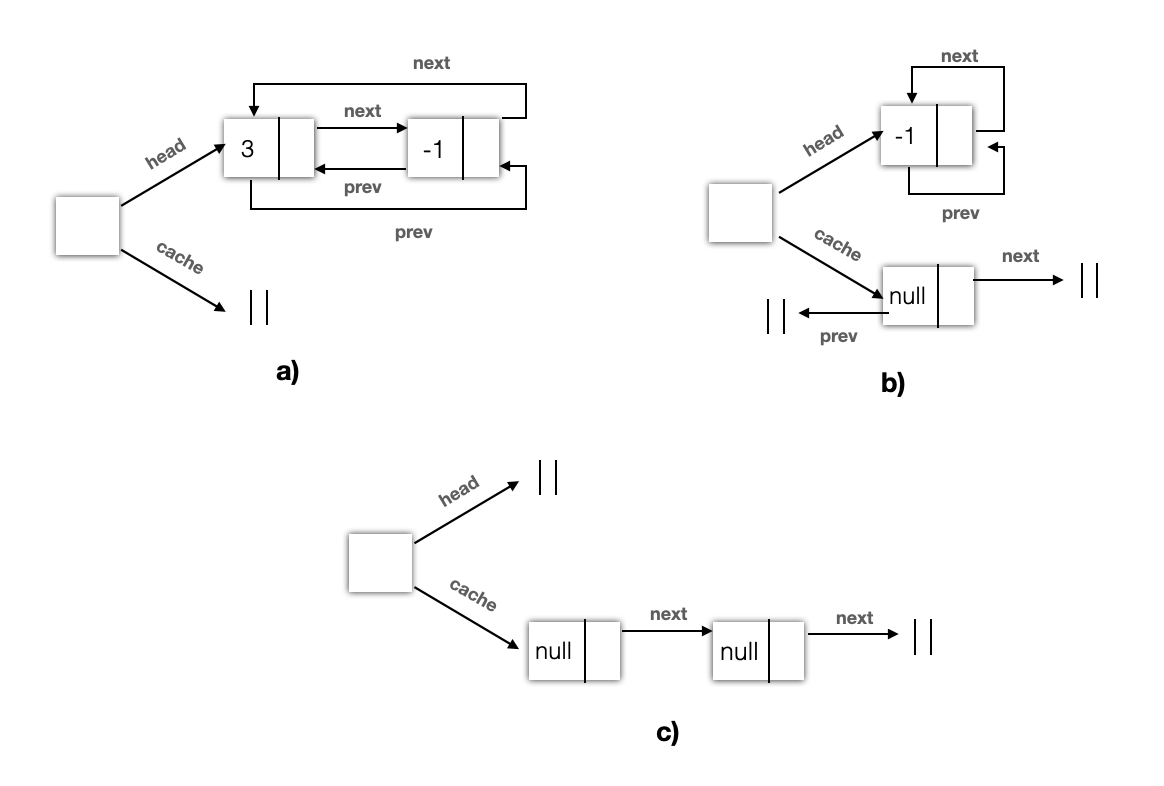
\includegraphics[width=1.0\textwidth]{images/ncl_instancias.png}
    \caption{Tres instancias de NodeCachingLinkedList con exactamente dos nodos.}
    \label{fig:ncl-instances-intro}
\end{figure}

\begin{itemize}
\item Figura (a): Esta instancia se construye agregando dos elementos a la lista
    principal, por ejemplo, ejecutando la siguiente secuencia de test:
\vspace{5pt} 
    \begin{lstlisting}[numbers=none,label=fig:NCLbuilders_a,xleftmargin=0pt]
    (0)  NodeCachingLinkedList();
    (7)  addFirst(3);
    (7)  addFirst(-1);
    \end{lstlisting}

\item Figura (b):
    \cacho{Esta instancia se logra agregando dos nodos a la lista principal y luego eliminar uno de ellos. En este caso el primero en agregar a la lista principal
    y se mueve el nodo a la lista cache}
    \vspace{5pt} 

    \begin{lstlisting}[numbers=none,label=fig:NCLbuilders_b, xleftmargin=0pt]
    (0)  NodeCachingLinkedList();
    (7)  addFirst(3);
    (7)  addFirst(-1);
    (25) removeFirst();
    \end{lstlisting}

\item Figura (c): 
    Esta instancia se genera añadiendo dos nodos al inicio y luego eliminándolos
    para pasarlos a la lista cache
    \vspace{5pt} 

    \begin{lstlisting}[numbers=none,label=fig:NCLbuilders_c, xleftmargin=0pt]
    (0)  NodeCachingLinkedList();
    (7)  addFirst(3); 
    (7)  addFirst(-11); 
    (25) removeFirst();
    (25) removeFirst();
    \end{lstlisting}
\end{itemize}



\section{Métodos Generadores de Objetos y sus Propiedades}

%\pp{Definición de generadores de objetos}
Se puede observar que, a pesar de que la API de NCL es muy compleja, como se observa en la Tabla~\ref{tab:ncl-api}, no todos los métodos son necesarios para construir objetos. 
Por ejemplo, combinaciones de los métodos mostrados en la Figura~\ref{fig:NCLbuilders}, con los parámetros adecuados, son suficientes para generar cualquier instancia de NCL.
\vspace{5pt} 
\begin{lstlisting}[numbers=none,label=fig:NCLbuilders, caption=Conjunto de métodos generadores de objetos para NCL]
  (0)  NodeCachingLinkedList()
  (7)  addFirst(Object)
  (25) removeFirst()
\end{lstlisting}

Una vez inicializada la instancia de NCL con el constructor, se pueden insertar elementos en la lista utilizando el método \texttt{addFirst}. Adicionalmente, el método \texttt{removeFirst} permite crear instancias que posean nodos en la lista caché (eliminando el nodo de la lista principal). 

De esta manera, los métodos de la Figura~\ref{fig:NCLbuilders} conforman un conjunto \emph{suficiente de métodos generadores de objetos}, es decir, son conjuntos de métodos que permiten generar todos los objetos posibles de NCL. Por simplicidad, llamaremos \emph{generadores de objetos} a estos métodos.

Notar que pueden existir distintos subconjuntos suficientes de generadores de objetos, como por ejemplo los que se muestran en las Figuras~\ref{fig:NCLbuilders2} y~\ref{fig:NCLnoMin1}. 
\vspace{5pt} 
\begin{lstlisting}[numbers=none,label=fig:NCLbuilders2, caption=Otros métodos generadores de objetos, frame=tb , basicstyle=\scriptsize, xleftmargin=0pt]
  (0)  NodeCachingLinkedList()
  (3)  add(Object)
  (25) removeFirst()
\end{lstlisting}


En particular, la Figura~\ref{fig:NCLnoMin1} contiene métodos \emph{superfluos}, es decir, métodos que pueden quitarse sin perder la propiedad de suficiencia del conjunto resultante. Por ejemplo, podemos eliminar \texttt{remove(Object)} y los métodos restantes siguen siendo generadores de objetos suficientes (similarmente, podríamos eliminar \texttt{removeFirst()}). 
\vspace{5pt} 

\begin{lstlisting}[numbers=none,label=fig:NCLnoMin1, caption=Métodos generadores de objetos suficientes pero no minimales, captionpos=b, frame=tb , xleftmargin=0pt, basicstyle=\scriptsize]
  (0)  NodeCachingLinkedList()
  (7)  addFirst(Object)
  (3)  remove(Object)
  (25) removeFirst()
\end{lstlisting}

Estamos interesados en conjuntos de métodos generadores de objetos \emph{minimales}, es decir, en conjuntos generadores de objetos suficientes con la menor cantidad posible de métodos. En otras palabras, los generadores de objetos son minimales si la exclusión de cualquiera de los métodos hace imposible la creación de ciertas instancias del módulo.
Así, las Figuras~\ref{fig:NCLbuilders} y ~\ref{fig:NCLbuilders2} muestran ejemplos de generadores de objetos suficientes y minimales.

Notar que muchos métodos en la tabla \ref{tab:ncl-api} están marcados como observadores (columna Obs?), lo que significa que no modifican los objetos sobre los que operan, ni son útiles para crear nuevos objetos. 
Debido a que estos métodos observadores siempre son superfluos y nunca deben incluirse en un conjunto de generadores de objetos minimal. Por esta razón, nuestros enfoques de identificación de métodos generadores intentan reconocerlos de antemano y descartarlos.

También, observamos que cuanto más fáciles de instanciar sean los parámetros de una rutina, usualmente la rutina será más eficiente de utilizar en el contexto de un análisis de programas (por ejemplo, para generar entradas para testing). Por ejemplo, entre las alternativas de rutinas para insertar datos en
la lista principal de NCL (ver Tabla~\ref{tab:ncl-api}), \texttt{add(int,Object)} recibe más parámetros que los otros tres métodos posibles. En cambio, \texttt{add(Object)}, \texttt{addFirst(Object)}, \texttt{addLast(Object)} toman un único parámetro. Si bien cualquiera de estas rutinas sirve para generar los mismos objetos de NCL, hay más formas de invocar a \texttt{add(int,Object)}. Esto usualmente redunda en una pérdida de eficiencia en la construcción de objetos por parte de un análisis automático de programas. Similarmente, elegiremos métodos con parámetros más simples (por ejemplo, parámetros de tipo primitivo), que otros con parámetros más complejos (por ejemplo, parámetros de tipo referencia) siempre y cuando los métodos permitan construir los mismos objetos.

De la discusión anterior se desprende que preferimos los métodos con menor número de parámetros, y con parámetros más fáciles de instanciar en los generadores de objetos (siempre que se mantengan las propiedades de suficiencia y minimalidad de los generadores). 
En nuestro ejemplo anterior, elegiremos \texttt{add(Object)} (o \texttt{addFirst(Object)} o \texttt{addLast(Object)}) en lugar de \\
\texttt{add(int,Object)} 
como parte de un conjunto suficiente y minimal de generadores de objetos.

Para concluir esta sección, es importante destacar que identificar manualmente un conjunto suficiente y minimal de métodos generadores de objetos es una tarea difícil y trabajosa, que requiere inspeccionar minuciosamente el código fuente del módulo y las formas en las que los métodos interactúan entre sí para generar objetos. Esto se dificulta aún más cuando los módulos cuentan con APIs ricas, como en nuestro ejemplo motivador (ver Tabla~\ref{tab:ncl-api}). 
Para facilitar la tarea del desarrollador, en las secciones siguientes proponemos enfoques automáticos para identificar conjuntos de métodos generadores de objetos.

\pp{Quizás esto sirva para explicar la explosión de combinaciones de métodos en los análisis de programas? Hay que pensarlo..} 
\pp{Pablo: Builders usage in program analyses? Now or later? We'll see...}

\section{Definiciones preliminares}
\label{sec:preliminares}


% Intro
En este capítulo, nos enfrentamos al desafío de identificar un conjunto suficiente y minimal de generadores de objetos a partir de la API de un módulo. 
Nos enfrentamos a un problema de optimización, donde apuntamos a encontrar el mejor estado según una función objetivo.
Esta definición es la de los algoritmos de búsqueda local \cite{Russell:2009}.
Para abordar este problema desarrollamos dos algoritmos de búsqueda, cada uno con su enfoque único. Estos algoritmos nos permiten explorar el espacio de búsqueda de manera eficiente y efectiva.

El primer algoritmo que presentamos es un enfoque basado en algoritmos genéticos, que utiliza principios inspirados en la evolución biológica. \cite{Goldberg:1989}
%, este algoritmo se enfoca en generar conjuntos de métodos generadores que puedan dar lugar a configuraciones más grandes y diversas de objetos. 
La naturaleza basada en la evolución de este enfoque permite encontrar soluciones prometedoras y adaptarse a diferentes situaciones.

El segundo algoritmo que proponemos es un enfoque \emph{greedy}, específicamente una variante de un algoritmo de ascenso de colinas \cite{Russell:2009,Cormen2009}. Este enfoque se centra en mejorar iterativamente un conjunto inicial de métodos generadores mediante la adición de métodos.
%, buscando siempre mejorar la calidad del conjunto en términos de eficiencia en cuanto a los objectos generados y la cobertura que se logra utilizando estos objectos sobre la API bajo test.

%Por último, presentamos un algoritmo basado en la idea de particionar los subconjuntos de métodos de la API en "clases de equivalencias" según los objetos que construyen. Esta estrategia nos permite agrupar métodos con propiedades similares y seleccionar conjuntos de métodos más cohesivos y efectivos.

Cada uno de estos algoritmos ofrece ventajas y desventajas en términos de rendimiento y precisión. Nuestra investigación se centró en comparar y evaluar estos algoritmos en diferentes casos de estudio para determinar cuál de ellos se adapta mejor a la tarea de identificar conjuntos suficientes y minimal de generadores de objetos.

% Para abordar estos desafíos planteados, a continuación se proponen dos enfoques para seleccionar automáticamente un conjunto suficiente y minimal de métodos generadores de objetos a partir de una API. El primero es un enfoque \emph{greedy}, basado en \emph{hill climbing}. El segundo enfoque utiliza algoritmos genéticos. En la próxima sección, explicaremos en detalle cada uno de estos enfoques y su implementación.

Por simplicidad, a partir de esta sección llamaremos generadores de objetos a aquellos que cumplan con las propiedades de suficiencia y minimalidad, ya que estamos interesados en identificar generadores de objetos con estas características.

% Observadores que es compartido por todos los algoritmos

\subsection{Identificación de métodos observadores}

 Los métodos observadores cumplen un papel fundamental en la API, ya que permiten inspeccionar el estado de un objeto. Estos métodos se caracterizan por no modificar el estado interno del objeto en cuestión. En otras palabras, su ejecución no altera ninguno de los atributos del objeto.
  También pueden usarse para verificar el estado de un objeto antes de realizar una operación que podría modificarlo.
 Por ejemplo, antes de eliminar un elemento de una lista, el método \texttt{isEmpty} de la lista puede ser utilizado para verificar si la lista contiene elementos. Si está vacía, se evita intentar una operación inválida.

Se puede observar en el código de la Figura \ref{fig:emptyObs} que las funciones \emph{isEmpty} y \emph{size} de la clase NodeCachingLinkedList (NCL) son métodos observadores.  Estos métodos no modifican ningún atributo de la clase NCL.
 
\begin{lstlisting}[language=Java, label=fig:emptyObs, caption=Algunos métodos observadores de la clase NCL. Se observa que no modifican el estado de NCL., captionpos=b, frame=tb]
public class NodeCachingLinkedList {
    Node head;
    int size;
    /**
      Devuelve verdadero si la lista esta vacia. 
    */ 
    public boolean isEmpty() { 
        return head == null; 
    }
    
    /**
      Devuelve el tamano de la lista. 
    */ 
    public int size() { 
        return size; 
    }
    
}
\end{lstlisting}


% En el ejemplo motivador presentado en la sección anterior y en la Tabla \ref{tab:ncl-api} se puede ver que existen muchos métodos clasificados como observadores. 
% Antes de ejecutar cualquiera de nuestros algoritmos, resulta fundamental identificar los métodos observadores. La razón principal es que estos métodos no contribuyen en la creación de nuevos objetos, ya que no sirven para construir objetos ni para modificar el estado de los objetos existentes. Por ende, no tienen ninguna utilidad en el contexto de los algoritmos de búsqueda de generadores de objetos.

% Para automatizar la identificación de métodos observadores, hemos utilizado una herramienta de análisis estático, \emph{Infer} \footnote{https://fbinfer.com/}, 
% desarrollada por Facebook. \emph{Infer} ofrece funcionalidades avanzadas que permiten analizar código fuente y clasificar métodos como observadores \cite{Huang:2012} (también denominados métodos puros en la bibliografía \cite{Huang:2012}).
% \emph{Infer} implementa la identificación de observadores mediante un análisis estático del código de los métodos \cite{Huang:2012,Salcianu:2005}. 
% Si bien el análisis de \emph{Infer} puede ser impreciso en algunos casos y generar falsos negativos (clasificar métodos como no observadores cuando si lo son), 
% en nuestros experimentos \emph{Infer}  identifica una buena proporción de los observadores de las APIs, lo que reduce significativamente el espacio de búsqueda de nuestros algoritmos.

% Entre las ventajas de utilizar \emph{Infer} se incluyen:

% \begin{itemize}
% \item \textbf{Eficiencia:} Automatiza el proceso de clasificación, ahorrando tiempo y esfuerzo manual.
% \item \textbf{Precisión:} Reduce el riesgo de errores humanos al identificar métodos irrelevantes para ciertos análisis.
% \item \textbf{Compatibilidad:} Es compatible con varios lenguajes de programación y puede integrarse en flujos de desarrollo modernos.
% \end{itemize}

% Por ejemplo, al analizar la API de NCL con \emph{Infer}, el resultado que
% obtenemos es el que se encuentra en la columna \emph{Observador?} de la tabla
% \ref{tab:ncl-api}.

\cacho{Es nuevo}
En el ejemplo motivador presentado en la Sección~\ref{sec:motivacionBuilders} y en la Tabla~\ref{tab:ncl-api}, se puede observar que existen numerosos métodos clasificados como observadores. 
Antes de ejecutar cualquiera de nuestros algoritmos, resulta fundamental identificar este tipo de métodos, ya que no contribuyen a la construcción de nuevos objetos: no modifican el estado del sistema ni crean nuevas instancias útiles para el objetivo. 
Por lo tanto, no tienen ninguna utilidad en el contexto de los algoritmos de búsqueda de métodos generadores de objetos, y pueden descartarse de forma segura.

Para automatizar la identificación de estos métodos, hemos utilizado la herramienta de análisis estático \emph{Infer}~\footnote{\url{https://fbinfer.com/}}, desarrollada por Facebook. 
\emph{Infer} ofrece funcionalidades avanzadas para analizar código fuente y clasificar métodos como observadores~\cite{Huang:2012} (también denominados \emph{métodos puros} en la bibliografía~\cite{Salcianu:2005}).
La clasificación se realiza mediante un análisis estático que infiere efectos secundarios sobre el estado de los objetos, sin necesidad de ejecutar el código.

Si bien \emph{Infer} puede generar falsos negativos —por ejemplo, no clasificar como observador a un método que en realidad sí lo es, como \texttt{iterator()}—, su comportamiento es conservador y evita falsos positivos. 
Es decir, rara vez clasificará como observador a un método que en realidad tiene efectos colaterales. 
Esta característica lo convierte en una herramienta extremadamente útil como filtro preliminar, su bajo costo computacional permite eliminar rápidamente una gran cantidad de métodos irrelevantes, 
lo que reduce de forma significativa el espacio de búsqueda de nuestros algoritmos sin comprometer la corrección del análisis.

La Tabla~\ref{tab:ncl-api} presenta la clasificación manual de los métodos de la clase 
\texttt{NodeCachingLinkedList}, distinguiendo cuáles se comportan como observadores y cuáles no, 
a partir del análisis de su implementación. 
Posteriormente, en la Tabla~\ref{tab:ncl-infer-comparacion} se muestra la comparación con el análisis 
automatizado realizado por \emph{Infer}. 
En esta segunda tabla, la columna adicional \emph{Infer} indica el resultado provisto por la herramienta, 
lo que permite identificar tanto los aciertos como las discrepancias respecto de la clasificación manual.

\begin{table}[H]
\centering
\scriptsize
\begin{tabular}{clcc}
\toprule
No. & Nombre del Método & Observador? & Infer \\
\midrule
0  & NCL()                        & no  & no \\
1  & NCL(int)                     & no  & no \\
2  & NCL(Collection)              & no  & no \\
3  & add(Object)                  & no  & no \\
4  & add(int,Object)              & no  & no \\
5  & addAll(Collection)           & no  & no \\
6  & addAll(int,Collection)       & no  & no \\
7  & addFirst(Object)             & no  & no \\
8  & addLast(Object)              & no  & no \\
9  & clear()                      & no  & no \\
10 & contains(Object)             & sí  & sí \\
11 & containsAll(Collection)      & sí  & sí \\
12 & equals(Object)               & sí  & sí \\
13 & get(int)                     & sí  & sí \\
14 & getFirst()                   & sí  & sí \\
15 & getLast()                    & sí  & sí \\
16 & indexOf(Object)              & sí  & sí \\
17 & isEmpty()                    & sí  & sí \\
18 & iterator()                   & no  & sí \\
19 & lastIndexOf(Object)          & sí  & si \\
20 & listIterator()               & no  & sí \\
21 & listIterator(int)            & no  & sí \\
22 & remove(int)                  & no  & no \\
23 & remove(Object)               & no  & no \\
24 & removeAll(Collection)        & no  & no \\
25 & removeFirst()                & no  & no \\
26 & removeLast()                 & no  & no \\
27 & retainAll(Collection)        & no  & no \\
28 & set(int,Object)              & no  & no \\
29 & size()                       & sí  & sí \\
30 & subList(int,int)             & sí  & sí \\
31 & toArray()                    & sí  & sí \\
32 & toArray(Object[])            & sí  & sí \\
33 & toString()                   & sí  & sí \\
\bottomrule
\end{tabular}
\caption{Comparación entre observadores de \texttt{NodeCachingLinkedList} identificados manualmente y por \emph{Infer}.}
\label{tab:ncl-infer-comparacion}
\end{table}

En términos generales, \emph{Infer} logra detectar correctamente la mayoría de los métodos observadores. 
No obstante, se observan algunos casos particulares. 
Por ejemplo, clasifica como observadores a los métodos que devuelven iteradores 
(\texttt{iterator()}, \texttt{listIterator()}, \texttt{listIterator(int)}). 
Si bien este criterio no es del todo incorrecto, ya que dichos métodos permiten inspeccionar 
la estructura de datos sin necesariamente modificarla, la clasificación resulta ambigua. 
En la práctica, los iteradores suelen considerarse como una interfaz de recorrido y no como observadores directos, 
ya que pueden exponer operaciones que alteran el estado interno de la colección 
(por ejemplo, la operación \texttt{remove()} del iterador). 
Esto explica por qué \emph{Infer} los clasifica como observadores,
a simple vista sólo devuelven un acceso para recorrer la colección, 
pero en realidad los iteradores también permiten operaciones que pueden modificarla 
de modo que no aseguran que el estado de la lista se mantenga inmutable.

Los métodos reportados como observadores por \emph{Infer} son descartados antes de comenzar la búsqueda de métodos generadores de objetos, y no se consideran en ninguna fase posterior del proceso.
En síntesis, \emph{Infer} actúa como una etapa de preprocesamiento que combina eficiencia y utilidad práctica: permite reducir el número de métodos a analizar, sin necesidad de intervención manual, manteniendo un nivel de precisión suficiente para nuestros casos de estudio.
\cacho{Capaz falte alguna referencia donde nos diga que pasa esto}
% De esta manera, \emph{Infer} es utilizado como paso previo a la ejecución de nuestros algoritmos. Los métodos reportados como observadores por \emph{Infer} se descartan antes de comenzar la búsqueda de métodos generadores de objetos.
\cacho{hasta aca}


% 1- estados o configuraciones del problema
\subsection{Estados}
\label{sec:estados}
En el contexto de los algoritmos de búsqueda local, los estados representan las diferentes configuraciones o situaciones posibles dentro del problema que se está resolviendo. Cada estado corresponde a un elemento en el espacio de búsqueda, definido como el conjunto de todas las posibles combinaciones o configuraciones que el algoritmo puede explorar para encontrar una solución.

La representación de los estados es un elemento clave para el éxito de los algoritmos de búsqueda, ya que determina el tamaño del espacio de búsqueda. 
% Una representación adecuada debe cumplir con los siguientes criterios:
% \begin{itemize}
%     \item \textbf{Relevancia:} Capturar todas las características esenciales del problema sin incluir información redundante o innecesaria.
%     \item \textbf{Eficiencia:} Permitir operaciones rápidas de expansión, evaluación y manipulación durante la búsqueda.
%     \item \textbf{Escalabilidad:} Adaptarse a problemas de mayor complejidad sin introducir un sobrecosto computacional significativo.
% \end{itemize}
Una representación demasiado compleja puede hacer que el algoritmo sea computacionalmente costoso y lento, mientras que una representación demasiado simplificada puede llevar a la pérdida de información importante, reduciendo la capacidad del algoritmo para encontrar soluciones óptimas.

%La codificación del espacio de búsqueda implica definir cómo se representan los estados y cómo se generan nuevos estados durante la exploración. 
En nuestros algoritmos de búsqueda, los estados están compuestos por subconjuntos de métodos de una API. Para representar estos subconjuntos, utilizamos vectores booleanos, donde cada posición en el vector indica si un método específico está incluido o no en el conjunto.

Como vimos en la tabla \ref{tab:ncl-api}, \texttt{NCL}, tiene un total de 34 métodos. Sin embargo, no todos estos métodos son relevantes para nuestros algoritmos. Por ejemplo, los métodos observadores deben excluirse del análisis ya que no contribuyen a la construcción de objetos. Esto reduce el número total de métodos considerados, lo que a su vez reduce significativamente el espacio de búsqueda.

Después de excluir los métodos observadores, quedan 20 métodos relevantes en NCL. Estos métodos se enumeran desde 0 hasta 19 como se puede observar en la tabla \ref{tab:ncl-api-infer}. 
\begin{table}[H]
\centering
{\scriptsize
\begin{tabular}{|l|l|}
\hline
No. & Nombre del Método \\
\hline
0  & NCL() \\
1  & NCL(int) \\
2  & NCL(Collection) \\
3  & add(Object) \\
4  & add(int,Object) \\
5  & addAll(Collection) \\
6  & addAll(int,Collection) \\
7  & addFirst(Object) \\
8  & addLast(Object) \\
9  & clear() \\
10 & iterator() \\
11 & listIterator() \\
12 & listIterator(int) \\
13 & remove(int) \\
14 & remove(Object) \\
15 & removeAll(Collection) \\
16 & removeFirst() \\
17 & removeLast() \\
18 & retainAll(Collection) \\
19 & set(int,Object) \\
\hline
\end{tabular}
}
\caption{API de NodeCachingLinkedList de Apache después de la identificación de métodos observadores.}
\label{tab:ncl-api-infer}
\end{table}


La representación de los estados en nuestros algoritmos se realiza mediante vectores booleanos. Cada posición $i$ en el vector representa el $i$-ésimo método de la API:

\[
c = [g_1, g_2, \ldots, g_n]
\]

donde:
\begin{itemize}
    \item $g_i = 1$ si el $i$-ésimo método está incluido en el subconjunto representado por el estado.
    \item $g_i = 0$ si el método no está incluido.
\end{itemize}

Por ejemplo, un estado posible puede representarse como un vector de la siguiente forma:


\begin{figure}[H]
  \centering
  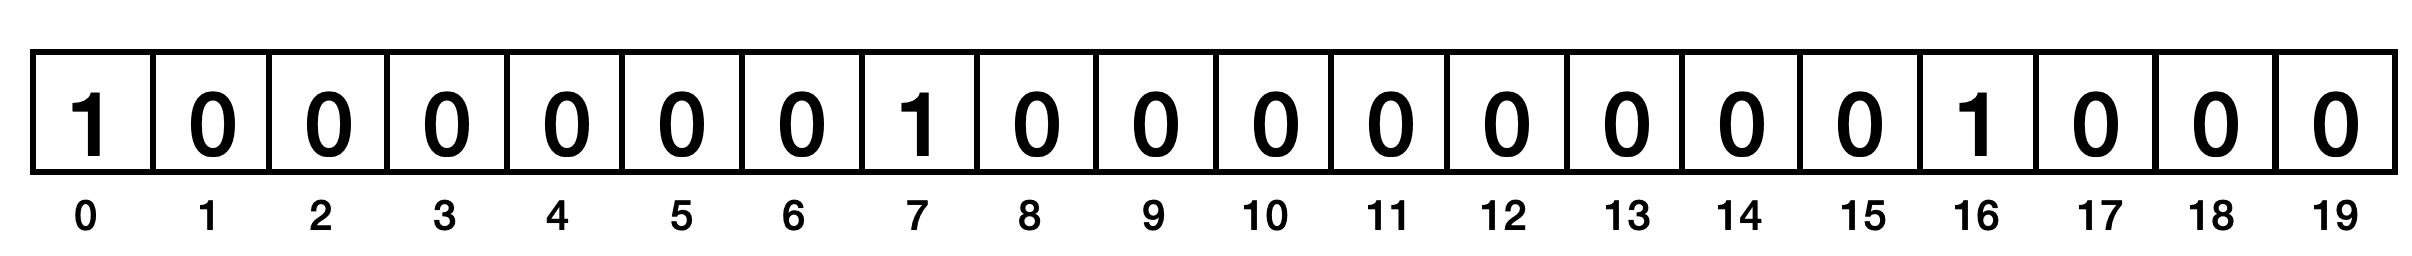
\includegraphics[width=1.0\textwidth]{images/cromosoma.png}
  \caption{Ejemplo de representacion de estado con un vector booleano}
  \label{fig:cromosoma}
\end{figure}

En este caso, las posiciones 0, 7 y 16 del vector están establecidas como verdaderas (según el orden asignado a los métodos de la API), mientras que las demás posiciones están establecidas como falsas. Esta configuración representa el subconjuto de métodos:
\vspace{5pt} 

\begin{lstlisting}[numbers=none, caption=Métodos generadores de objetos que representa el cromosoma de la Figura \ref{fig:cromosoma}, captionpos=b, frame=tb , xleftmargin=0pt, basicstyle=\scriptsize]
  (0)  NodeCachingLinkedList()
  (7)  addFirst(Object)
  (16) removeFirst()
\end{lstlisting}

\section{Funciones objetivo}
\label{sec:fitness}
% 2- función de valoración
% también denominada función de aptitud en algoritmos genéticos

Una función objetivo, también conocida como función de costo o función de valoracion, es una función matemática que mide la calidad de una solución candidata dentro del espacio de búsqueda \cite{Russell:2009}. Esta función asigna un valor numérico a cada estado, indicando qué tan buena o deseable es el candidato con respecto al objetivo del problema.

El propósito de la función objetivo es guiar el proceso de búsqueda hacia la mejor solución posible. Dependiendo del problema, se busca maximizar o minimizar el valor de la función. En problemas de maximización, se priorizan los estados con valores más altos, mientras que en problemas de minimización, se favorecen aquellos con valores más bajos.

La función objetivo es una parte fundamental de los algoritmos de búsqueda local. Estos algoritmos utilizan la función objetivo para evaluar y comparar diferentes estados candidatos a medida que exploran el espacio de búsqueda en busca de la mejor solución posible.

En nuestros algoritmos, hemos desarrollado dos funciones objetivo distintas para guiar el proceso de búsqueda. 
Cada una de ellas con su enfoque para evaluar y comparar diferentes configuraciones de métodos generadores de objetos.

Como el conjunto de objetos que se pueden construir con la API de un módulo es potencialmente infinito, las funciones objetivo definidas a continuación usan diferentes mecanismos para acotar el espacio de búsqueda.


\subsection{Generación Exhaustiva Acotada}
\label{sec:fitnessGE}

Dado un candidato $C$ que representa un subconjunto de métodos $M$ de la API, 
nuestra función objetivo intenta calcular el número de objetos que se pueden construir utilizando combinaciones de métodos en $M$. 
Los candidatos con valores de aptitud más altos se estima que construyen más objetos que aquellos que tienen valores de aptitud más pequeños.

Así, la primera función objetivo propuesta evalúa la capacidad de generación de objetos de un candidato $C$ realizando una generación exhaustiva acotada \cite{Politano20} usando los métodos en $M$. La función objetivo asigna un puntaje a $C$ basándose en la cantidad de objetos únicos producidos durante la generación exhaustiva acotada. Esto refleja la diversidad de objetos que se pueden generar utilizando los métodos dados. Los subconjuntos de métodos que generan más objetos serán los candidatos preferidos para ser elegidos por nuestro algoritmo como generadores de objetos.
Nuestro enfoque utiliza un generador exhaustivo acotado eficiente basado en métodos de la API \cite{Politano20}. Este generador se denomina BEAPI y es una de las contribuciones principales de este trabajo (ver Capítulo \ref{cap:beapi}).
Dado un conjunto de métodos $M$ en un candidato $C$, BEAPI explora todas las secuencias de métodos acotadas que se pueden construir usando métodos de $M$. La cota consiste de un número máximo $m$ de métodos dado por el usuario, y de un conjunto de valores primitivos empleados para instanciar los parámetros de tipo primitivo en los métodos en $M$ (e.g., enteros de \( 0 \) a \( k-1 \)).
BEAPI utiliza cada uno de estos valores para instanciar cada parámetro del tipo correspondiente. 
BEAPI cuenta la cantidad de objetos distintos creados por la ejecución de cada una de las secuencias exploradas. 
Así, para $M$ (y cotas $m$ y $k$) la función objetivo retorna el número de objetos generados por BEAPI usando $M$.

Como la cantidad de secuencias a explorar crece exponencialmente respecto de las cotas, BEAPI implementa distintas técnicas que le permiten podar significativamente el espacio de búsqueda y mejorar la eficiencia de la generación (usar el feedback de la ejecución para descartar secuencias inválidas, coincidencia de estado para evitar volver a generar repetidamente los mismos objetos, descartar secuencias que generen objetos de tamaño mayor al permitido por las cotas). Para obtener más información sobre las mismas y sobre BEAPI invitamos al lector a consultar el Capítulo \ref{cap:beapi}.

Nuestra técnica se basa en una variante de la \emph{hipótesis de la cota pequeña}, ampliamente reconocida en el testing de software \cite{Andoni:2003,jackson2006, Abad13}. La hipótesis de la cota pequeña indica que la mayoría de las fallas pueden revelarse ejercitando el software bajo test con entradas de tamaño relativamente pequeño. Nuestra hipótesis es que si dos conjuntos de métodos $M_1$ y $M_2$ generan los mismos objetos acotados (para una cota relativamente pequeña), entonces es altamente probable $M_1$ y $M_2$ sirvan para generar los mismos objetos en un contexto no acotado. Esto fue validado empíricamente en todos nuestros casos de estudio.

\begin{lstlisting}[label=fig:rankParameters,caption=Ranking con los tipos de parametros, captionpos=b,frame=tb, float=t]
Boolean=1
Integer,Char=2
Float,Double,String=4
Object=6
\end{lstlisting}

Como ya se discutió en esta Sección, buscamos un conjunto minimal de generadores de objetos, donde los métodos tengan parámetros tan simples como sea posible. Por lo tanto, la cantidad de objetos generados usando BEAPI es sólo un componente de la función objetivo. Dado un conjunto de métodos $M$, la función objetivo $f$ devuelve un valor real conformado por tres componentes:

\[
f(M) = \langle O(M), R(M), P(M) \rangle
\]
Donde:

\cacho{Lo de parametros lo agrego PP, lo dejo}
\begin{itemize}
    \item $O(M)$ (Objetos): Es el número de objetos generados por el conjunto de métodos $M$ usando generación exhaustiva acotada, para un scope fijo. Este componente es el más importante, ya que los siguientes componentes sólo se usan para decidir en caso de empate respecto de $O(M)$. Recordemos que los generadores de objetos a identificar deben ser siempre suficientes, por lo que la función objetivo siempre prioriza los métodos que generen un mayor número de objetos.
    \item $R(M)$ (Redundancia): Representa la diferencia entre el número total de métodos de la API ($M_t$) y la cantidad de métodos en $M$. Esto se utiliza para desempatar entre conjuntos de métodos que generan la misma cantidad de objetos, dando preferencia a aquellos conjuntos que contengan menos métodos. En otras palabras, este componente de la función busca identificar generadores de objetos minimales.
        de modo que, para un $M_t$, $R(M)$ es equivalente a $\#M_t - \#M$.
    \item $P(M)$ (Parámetros): Es una medida ponderada de la complejidad de los
        parámetros de los métodos en $M$. Sea $m_l$ un método con parámetros $p_1: T_1,
            p2: T_2, \ldots, p_k: T_j$, la función $W(m_l)$ define el peso de los
            parámetros de $m_l$ de acuerdo al tipo de los mismos. $W$ se
            define como: $W(m_l) = \sum_{i=1}^j = T(T_i)$, donde $T$ es la función
            definida en la Tabla \ref{fig:rankParameters}, que asigna a cada
            tipo un valor predefinido. $T$ es una función definida de manera heurística, 
            que asigna un mayor peso a tipos más complejos. $T$ se definió 
            considerando pesos para los tipos que dieron buenos resultados en
            nuestra evaluación experimental, y podría reemplazarse de manera
            directa por mejores heurísticas en el futuro. Extendemos la
            definición de $W$ para conjuntos de métodos de la siguiente manera.
            Sea $M'$ un subconjunto de métodos, $W(M') = \sum_{m \in M'} W(m)$.
            Si $API$ es el conjunto total de métodos, $W(API)$ representa
            el peso máximo que podría tener un subconjunto (el conjunto que
            incluye todos los métodos). 
            Ahora estamos listos para definir $P$. Como buscamos maximizar $P$, 
            primero computaremos $W(API)$ y le restaremos el valor de $W(M)$. 
            Esto es, $P(M) = W(API) - W(M)$. Esta componente de $f(M)$ se
            utiliza para desempatar entre conjuntos de métodos que generan la
            misma cantidad de objetos y tienen la misma cantidad de métodos,
            favoreciendo subconjuntos con una menor complejidad en sus
        parámetros.


\end{itemize}


A partir de esto, podemos definir un orden sobre esta función $f$, sean dos
métodos $M_1$ y $M_2$ tales que: 

\( f(M_1) = \langle O(M_1), R(M_1), P(M_1) \rangle \) y

\( f(M_2) = \langle O(M_2), R(M_2), P(M_2) \rangle \) 
\vspace{5pt} 

el orden se define de la siguiente forma:

\[
f(M_1) > f(M_2) \quad \text{si y solo si:}
\]

\begin{enumerate}
    \item \( O(M_1) > O(M_2) \), o
    \item \( O(M_1) = O(M_2) \) y \( R(M_1) > R(M_2) \), o
    \item \( O(M_1) = O(M_2) \), \( R(M_1) = R(M_2) \), y \( P(M_1) > P(M_2) \).
\end{enumerate}

En otras palabras, se compara primero el número de objetos \( O(M_1) \) con \( O(M_2) \). 
Si son iguales, se compara la redundancia \( R(M_1) \) con \( R(M_2) \), y si ambos son iguales, 
se compara la complejidad de los parámetros \( P(M_1) \) con \( P(M_2) \).

Para ilustrar este concepto, consideremos los siguientes ejemplos.


En el primer caso, analizamos dos conjuntos de métodos:

\vspace{5pt}

\begin{lstlisting}[numbers=none, caption=Conjunto de métodos \( M_1 \)]
  NodeCachingLinkedList()
  addFirst(Object)
  removeFirst()
\end{lstlisting}

\begin{lstlisting}[numbers=none, caption=Conjunto de métodos \( M_2 \)]
  NodeCachingLinkedList()
  addFirst(Object)
\end{lstlisting}


\cacho{Es nuevo esto}


Ambos conjuntos tienen en común el método \texttt{addFirst(Object)}, cuyo único parámetro es de tipo Object, 
con peso 6 según la Tabla~\ref{fig:rankParameters}. 
Los demás métodos no tienen parámetros, por lo tanto:

\[
W(M_1) = W(M_2) = 6
\]

Como el peso total de la API es 72, se obtiene:

\[
P(M_1) = P(M_2) = 72 - 6 = 66
\]

La API contiene un total de 20 métodos (ver Tabla~\ref{tab:ncl-api-infer}). Como \( M_1 \) utiliza 3 de ellos y \( M_2 \) solo 2, se obtiene:

\[
R(M_1) = 20 - 3 = 17 \quad \text{y} \quad R(M_2) = 20 - 2 = 18
\]

En nuestros experimentos (con un \emph{scope} igual a 3), \( M_1 \) genera 18 objetos, mientras que \( M_2 \) genera 12. Las funciones objetivo son entonces:

\[
f(M_1) = \langle 18, 17, 66 \rangle \quad \text{y} \quad f(M_2) = \langle 12, 18, 66 \rangle
\]

Dado que \( M_1 \) genera más objetos, se concluye que:

\[
f(M_1) > f(M_2)
\]

Esto implica que \( M_1 \) es un conjunto generador más adecuado, ya que permite construir un mayor número de instancias. 
En particular, \( M_2 \) no puede generar aquellas instancias que requieren eliminar elementos de la lista, lo cual sí permite \( M_1 \) mediante el método \texttt{removeFirst()}.


En el segundo caso, ambos conjuntos generan la misma cantidad de objetos (18, para scope 3), pero el conjunto \( M_4 \) incluye un método adicional:

\vspace{5pt}

\begin{lstlisting}[numbers=none,label=fig:NCLbuilders3, caption=Conjunto de métodos \( M_3 \)]
  NodeCachingLinkedList()
  addFirst(Object)
  removeFirst()
\end{lstlisting}

\begin{lstlisting}[numbers=none,label=fig:NCLbuilders4, caption=Conjunto de métodos \( M_4 \)]
  NodeCachingLinkedList()
  addFirst(Object)
  add(Object)
  removeFirst()
\end{lstlisting}

Las triplas resultantes son:

\[
f(M_3) = \langle 18, 17, 66 \rangle \quad \text{y} \quad f(M_4) = \langle 18, 16, 66 \rangle
\]

Ambos conjuntos logran generar la misma cantidad de objetos y presentan la misma complejidad en sus parámetros. Sin embargo, \( M_4 \) utiliza un método más, por lo que tiene una redundancia mayor (\( R(M_4) = 16 \) frente a \( R(M_3) = 17 \)). 
Dado que nuestra función objetivo favorece subconjuntos más reducidos en caso de empate, se concluye que:

\[
f(M_3) > f(M_4)
\]


En el tercer caso, los conjuntos tienen la misma cantidad de objetos generados (18, para scope 3) y el mismo número de métodos, pero difieren en la complejidad de los parámetros utilizados:

\begin{lstlisting}[numbers=none,label=fig:NCLbuilders5, caption=Conjunto de métodos \( M_5 \)]
  NodeCachingLinkedList()
  addFirst(Object)
  removeFirst()
\end{lstlisting}

\begin{lstlisting}[numbers=none,label=fig:NCLbuilders6, caption=Conjunto de métodos \( M_6 \)]
  NodeCachingLinkedList()
  add(int, Object)
  removeFirst()
\end{lstlisting}

Las triplas correspondientes son:

\[
f(M_5) = \langle 18, 17, 66 \rangle \quad \text{y} \quad f(M_6) = \langle 18, 17, 64 \rangle
\]

Ambos conjuntos tienen igual número de métodos y generan la misma cantidad de objetos. 
Sin embargo, \( M_6 \) contiene un método con parámetros más complejos (el método \texttt{add(int, Object)}) lo cual se refleja en un mayor peso de parámetros. 
Como la función \( f \) prefiere subconjuntos con menor complejidad de parámetros en caso de empate, se concluye que:

\[
f(M_5) > f(M_6)
\]

\cacho{hasta aca}


%Para este propósito, desarrollamos la herramienta BEAPI, que se discute con más detalle en el Capítulo \ref{cap:beapi}. En resumen, primero exploramos exhaustivamente todas las posibles combinaciones de secuencias de los métodos de $M$. Luego, utilizamos un conjunto fijo de valores primitivos (enteros del 0 a $k-1$) con los cuales probar nuestros métodos cuando requieren valores primitivos.

%En segundo lugar, descartamos las secuencias de métodos que crean objetos con más de $k$ objetos (de cualquier tipo) para evitar construir objetos más grandes de lo necesario. Para lograr esto, canonizamos los objetos generados por la ejecución de cada secuencia y descartamos la secuencia si algún objeto tiene un índice igual o mayor que $k$.

%En tercer lugar, ampliamos esta generación con coincidencia de estado. Esto se debe a que, en la generación de pruebas, a menudo hay muchas secuencias de pruebas que producen el mismo objeto. Por ejemplo, insertar en una colección y luego eliminar el mismo elemento resulta en muchos casos en exactamente la misma estructura antes de la inserción. Nuestro enfoque asume que las ejecuciones de rutinas son deterministas con respecto a sus entradas. Bajo esta suposición, se deduce que, para generar un conjunto exhaustivo acotado de estructuras, solo necesitamos guardar una secuencia de prueba para crear cada estructura diferente en el conjunto, y que todas las siguientes secuencias de prueba que generen la misma estructura se pueden descartar.


\subsection{Cobertura de código}
\label{sec:fitnessRandoop}

\cacho{La primer oracion lo agrego PP, lo dejo}
Como la generación exhuastiva acotada puede ser costosa computacionalmente,
proponemos aquí una heurística para computar la función objetivo que debería
dar lugar a una mejor eficiencia en los algoritmos de cómputo de métodos
generadores. Así, la segunda función objetivo se basa en generar test suites
de manera automática (aleatoria) utilizando un suconjunto candidato de métodos,  
y medir la cobertura de código que alcanzan estas test suites. 
La cobertura se mide en términos de las líneas de código y las ramas del
programa que son ejercitadas por los tests (\ref{sec:coverage}).
Esta métrica estima en qué medida los tests generados a partir del subconjunto de métodos cubren las distintas partes del programa, 
lo que permite valorar un aspecto clave de la calidad de las suites de test obtenidas.
% PABLO: Esto está en background
%Los criterios de evaluación incluyen:
%\begin{itemize}
%    \item \textbf{Cobertura de líneas de código:} Porcentaje de líneas de código ejecutadas al correr los test suites.
%    \item \textbf{Cobertura de ramas:} Porcentaje de decisiones (\textit{branches}) exploradas en el flujo de ejecución del programa.
%\end{itemize}
Por ejemplo, si se genera una test suite que cubre 100 líneas de código y 20 ramas de la API, 
la función objetivo combina estas métricas en un puntaje compuesto.

Para ello, se calcula la proporción de líneas y ramas cubiertas respecto del total disponible, 
y se ponderan según su importancia relativa. Así, la cobertura alcanzada por una
test suite puede definirse como:

\[
\text{Cob}(M) = \alpha \cdot \frac{L_M}{L_{\text{total}}} + \beta \cdot \frac{B_M}{B_{\text{total}}}
\]

donde $\alpha$ es $0.4$ y $\beta$ es $0.6$ para darle un peso mas importante a la cobertura de ramas.
Este enfoque es especialmente útil en casos donde el objetivo es favorecer
métodos que sean útiles para generar tests que ejerciten la mayor cantidad
posible de ramas del código.
En el contexto de nuestra tesis, hemos realizado modificaciones en la
herramienta \emph{Randoop} (descrita en la sección
\ref{sec:feedback-directed-test-gen})
de manera que las test suites generadas sean de utilidad para averiguar si un conjunto de 
métodos dados es un buen conjunto de métodos generadores.

La heurística para averiguar si un
subconjunto de métodos $M$ es un buen conjunto de generadores se basa en
realizar una primera ejecución de Randoop utilizando sólo los métodos en $M$ para
generar un conjunto de secuencias de test que generen objetos $tests_{obj}$. En
otras palabras, se asume que los métodos en $M$ son generadores de objetos (y
en la segunda etapa se busca evaluar si efectivamente lo son).
Luego, estas secuencias se extienden en una ejecución de Randoop subsiguiente,
pero esta vez usando los métodos restantes de la API. El objetivo de esta
segunda ejecución es maximizar la cobertura de código obtenida por la suite. 
De esta manera, si los métodos en $M$ son un buen conjunto de generadores de objetos
la cobertura obtenida por la suite final será alta; en caso contrario será baja. 
Por ejemplo, si la primera ejecución no puede construir muchos objetos, extender 
$tests_{obj}$ no dará lugar a buena cobertura.

El algoritmo de Randoop modificado para la detección de métodos generadores se muestra 
en la Figura \ref{alg:fitnessRandoop}.
Primero, se realiza una ejecución de Randoop sólo con los métodos de $M$ para
generar secuencias de test, $tests_{obj}$ (línea 6), que usan estos métodos para construir objetos \pp{Tiene state
matching activado esto?}. Esta ejecución utiliza un 40\% del tiempo total
asignado, \texttt{S} (ver $S_1$ en la línea 2). 
La función \texttt{GenerarNuevasSecuencias} (líneas 9-35) es la encargada de
producir estas secuencias de test. Esta función realiza su tarea utilizando 
la estrategia de generación aleatoria descrita en la Sección~\ref{sec:feedback-directed-test-gen}, basada en el enfoque de Randoop. 

\clearpage
\begin{algorithm}[H]
    \small
    \SetAlgoLined
    \KwIn{Métodos de la API $API$, subconjunto de métodos $M \subseteq API$,
    tiempo total $S$}
    \KwOut{Conjunto final de tests generados}
    
    \SetKwFunction{FMain}{GenerarTest}
    \SetKwFunction{FGen}{GenerarNuevasSecuencias}
    \SetKwProg{Fn}{Function}{:}{}
    \BlankLine


    \Fn{\FMain{$API$, $M$, $S$}}{
    
        $S_1 \leftarrow 0.4 \cdot S$\;
        $S_2 \leftarrow 0.6 \cdot S$\;
    
        $M_{gen} \leftarrow$ $M$\;
        $M_{nogen} \leftarrow$ $API - M$\;
    
        $tests_{obj}, tests_1 \leftarrow$ \FGen{$M_{gen}$, $S_1$}\;
        $prev_2, tests_2 \leftarrow$ \FGen{$M_{nogen}$, $S_2$, $tests_{obj}$}\;
    
        \Return{$tests_2$}\;
    }
    
    \BlankLine

    \Fn{\FGen{$M'$, $S'$, $T_0$}}{

    $tests \leftarrow \emptyset$\;
    $prev \leftarrow T_0$\;

    \While{tiempo transcurrido $< S'$}{
        Seleccionar aleatoriamente $m(p_1:T_1, \ldots, p_m:T_m) \in M'$\;
        \For{$p_i:T_i$ de $m$}{
            \If{$T_i$ es primitivo}{
                $S_i \leftarrow$ valor primitivo para $T_i$ tomado
                aleatoriamente de las semillas\;
            }\Else{
                $S_i \leftarrow$ secuencia aleatoria $\in prev$ que crea objeto de tipo $T_i$\;
            }
        }
        $test \leftarrow S_1; \ldots; S_m; m(v_1,\ldots,v_m)$\;
        $res \leftarrow ejecutar($test$)$\;
        \If{res = falla} {
            \Return{$\{ test \}$}\;
        }   
        \If{res = inválido} {
            // No se guarda test para futuras extensiones
        }       
        \If{res = exito} {
            $prev \leftarrow prev \cup \{test\}$\;
        }        
        $tests \leftarrow tests \cup \{test\}$\;
    }
    \Return{$tests$}\;
    }
    
    \caption{Generación de tests para cobertura de código}
    \label{alg:fitnessRandoop}
    \end{algorithm}
    

Más adelante, se realiza una segunda ejecución
de Randoop usando las secuencias de test $tests_{obj}$ como punto de partida para
generar otras secuencias nuevas, utilizando los restantes métodos de la API
($API - M$; ver línea 5). El resultado de esta ejecución es la suite de tests final
$tests_2$ (línea 7), retornada por el algoritmo (línea 8).
La segunda ejecución usa un 60\% del tiempo
asignado \texttt{S} (ver $S_2$ en la línea 3). 
Nuevamente, la producción de secuencias de test se hace invocando a
\texttt{GenerarNuevasSecuencias}.

Usamos el algoritmo \ref{alg:fitnessRandoop} para computar $Cob$ de la siguiente manera.
Primero, se genera una test suite para un conjuto de métodos dado $M$, con un tiempo límite
de generación $S$ fijo (determinado experimentalmente). Luego, se mide  
 la cobertura de líneas y de ramas obtenida por la test suite, y se computa
 $Cob$ aplicando la fórmula \ref{} \pp{poner fórmula} con estos valores.

La función objetivo que utilizamos para evaluar la calidad de un candidato, 
representado por un conjunto de métodos $M$, se define como una tripla al igual 
que la función de la sección \ref{sec:fitnessGE}.

\[
f'(M) = \langle Cob(M), R(M), C(M) \rangle
\]

Donde:

\begin{itemize}
    \item $Cob(M)$ (Cobertura): Es el número de ramas y lineas cubiertas
        (\ref{sec:coverage}) por la
        suite generada por el algoritmo \ref{alg:fitnessRandoop}, utilizando $M$ como
        entrada. 
    Este componente tiene la mayor importancia, ya que refleja directamente la
    efectividad de los tests al cubrir líneas y ramas de la API.
\item $R(M)$ (Redundancia): Diferencia entre el número total de métodos de la
    API ($M_t$) y la cantidad de métodos en $M$. Se define igual que para la
    función objetivo basada en generación exhuastiva acotada de la sección \ref{sec:fitnessGE}.
    \item $P(M)$ (Parámetros): Medida ponderada de la complejidad de los
        parámetros de los métodos en $M$. También mantuvimos el mismo cálculo
        que para la función objetivo basada en generación exhaustiva acotada.
\end{itemize}

Volvamos al ejemplo que usamos durante este capítulo. Consideremos los siguientes conjuntos de métodos:

\begin{lstlisting}[numbers=none, caption=Conjunto de métodos \( M_1 \)]
  NodeCachingLinkedList()
  addFirst(Object)
  removeFirst()
  
\end{lstlisting} 


\begin{lstlisting}[numbers=none, caption=Conjunto de métodos \( M_2 \)]
  NodeCachingLinkedList()
  addFirst(Object)

   
\end{lstlisting}


\cacho{Nuevo esto:}
Al ejecutar el algoritmo~\ref{alg:fitnessRandoop} con cada conjunto como entrada, se generan suites de tests que luego son evaluadas utilizando herramientas de análisis de cobertura. 
El resultado, expresado como la tripla \( \langle Cob, R, P \rangle \), se detalla a continuación:

\[
f(M_1) = \langle 293, 17, 66 \rangle \quad \text{y} \quad f(M_2) = \langle 272, 18, 66 \rangle
\]

En este caso, la cobertura  (\(Cob\)), se computa como la suma del número de líneas y ramas cubiertas.
Para \( M_1 \), se cubrieron 192 líneas y 101 ramas (\(Cob = 293\)), para \( M_2 \), se cubrieron 175 líneas y 97 ramas (\(Cob = 272\)).

Para la redundancia de métodos, tal cual la seccion anterior, se define como \( R(M) = M_t - |M| \), donde \( M_t \) es el número total de métodos en la API (en este caso, 20. Ver \ref{tab:ncl-api-infer}). 
El conjunto \( M_1 \) contiene 3 métodos, por lo que \( R(M_1) = 20 - 3 = 17 \) y el conjunto \( M_2 \) contiene 2 métodos, entonces \( R(M_2) = 20 - 2 = 18 \).

En cuanto a los parámetros, ambos conjuntos tienen la misma complejidad de parámetros, ya que ambos conjuntos incluyen únicamente el método \texttt{addFirst(Object)}, cuyo único parámetro es de tipo \texttt{Object}, con un peso de 6 según la Tabla~\ref{fig:rankParameters}. 
Los demás métodos no tienen parámetros. Por lo tanto, el peso total de parámetros en ambos conjuntos es \( W(M_1) = W(M_2) = 6 \), y como el peso total de la API es \( W(API) = 72 \), se obtiene \( P = 72 - 6 = 66 \) en ambos casos.

En este caso, el conjunto \( M_1 \) logra una mejor cobertura, lo cual alcanza este valor para elegirlo como mejor candidato. 
Esto se debe a que la inclusión de métodos como \texttt{removeFirst()} en \( M_1 \) permite generar tests más variados, que ejercitan comportamientos adicionales de la API. 
En contraste, \( M_2 \) no permite generar escenarios que modifiquen el estado interno de la lista, lo que impide alcanzar ciertas ramas del código.

Por lo tanto, de acuerdo con la función objetivo basada en cobertura, se prefiere el conjunto \( M_1 \):

\[
f(M_1) > f(M_2)
\]


En nuestra evaluación experimental, ambas funciones objetivo son utilizadas como
parte de los algoritmos de búsqueda implementados, para analizar sus ventajas y
desventajas en la práctica. 


\cacho{hasta aca}

\section{Algoritmos para la Identificación de Métodos Generadores de Objetos}
\label{sec:algorithms}
\cacho{Nuevo esto:}

En esta sección presentamos el proceso completo para identificar automáticamente métodos generadores de objetos a partir de la clase objetivo (target class). 
La Figura~\ref{fig:builders-overview} muestra una visión general del enfoque propuesto.

\cacho{Debo charlar con PP para ver la imagen y mejorarla. Creo que queda mejor al principio de todo el capitulo. Falta mejorar nombres en la imagen pero es para tener una idea}

\begin{figure}[H]
  \centering
  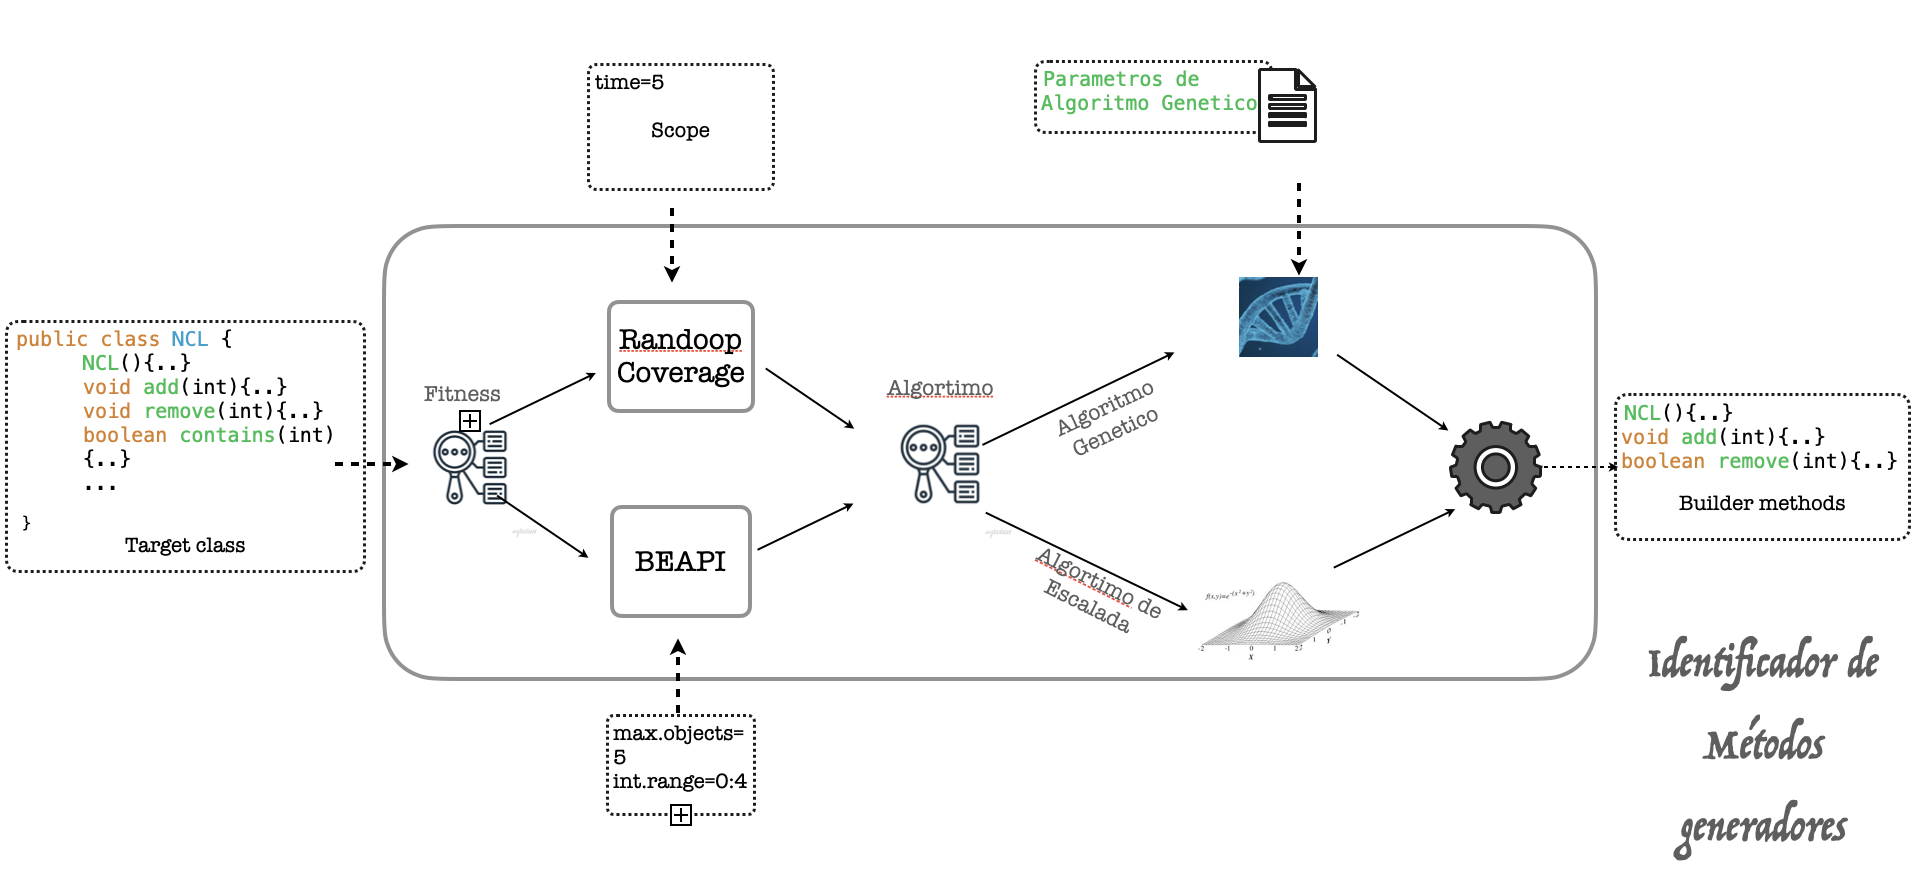
\includegraphics[width=1.0\textwidth]{images/builders.png}
  \caption{Framework de BEAPI}
  \label{fig:builders-overview}
\end{figure}


Dado una clase objetivo (por ejemplo, \texttt{NCL}), nuestro enfoque busca identificar el subconjunto de métodos de su API que permite construir objetos representativos, de acuerdo con un criterio de evaluación. 
Este proceso se estructura en tres componentes principales: la definición de una función objetivo, la exploración del espacio de soluciones mediante algoritmos de búsqueda, 
y la evaluación sobre dos variantes: generación exhaustiva acotada (usando BEAPI) y generación de tests (usando Randoop).

El procedimiento comienza con la especificación de la clase objetivo y los parámetros de configuración para el generador BEAPI (por ejemplo, el \texttt{scope}, el número máximo de objetos, y el rango de valores enteros permitidos). 
En paralelo, se pueden definir los parámetros del algoritmo genético o del algoritmo de escalada empleados para explorar el espacio de soluciones.

El sistema evalúa candidatos (subconjuntos de métodos) mediante una función objetivo que mide su capacidad para generar objetos válidos (en el caso de BEAPI), o para cubrir líneas y ramas del código (en el caso de Randoop).
Esta evaluación se traduce en una tripla que combina métricas como la cantidad de objetos generados o la cobertura alcanzada, junto con aspectos estructurales como la redundancia del conjunto y la complejidad de los parámetros de los métodos utilizados.

Los candidatos se refinan iterativamente utilizando algoritmos de búsqueda metaheurísticos. 
Finalmente, el mejor conjunto identificado se reporta como el conjunto de métodos generadores.

\cacho{hasta aca}

\subsection{Algoritmo Genético}
\label{alg:approachGA}

Los algoritmos genéticos \cite{Goldberg:1989} son algoritmos de búsqueda guiada no exhaustivos, 
basados en una estrategia de ascenso de colinas \cite{Russell:2009}. El espacio de búsqueda está 
compuesto por un conjunto generalmente muy grande de individuos (los candidatos), y
el objetivo de la búsqueda es encontrar un individuo con las características deseadas. 
A diferencia de los algoritmos de búsqueda clásicos, los algoritmos genéticos mantienen un conjunto de individuos,
llamado población, y la búsqueda progresa seleccionando iterativamente un número de individuos de la población, 
utilizando estos para la evolución (construyendo nuevos individuos a partir de estos), 
y dejando fuera algunos individuos del conjunto total (los ``viejos'' y los ``nuevos'').
La selección de individuos para la evolución de la población, así como la eliminación de individuos, 
son guiadas por una función objetivo, la función heurística utilizada para guiar la búsqueda. 
Esta función se aplica a los individuos, y su resultado es generalizable también a la población 
(por ejemplo, la aptitud de la población puede tomarse como la aptitud de su individuo "más apto").
Esta función captura las características deseadas en la búsqueda, y por lo tanto puede usarse como un 
criterio de detención (por ejemplo, el algoritmo se detiene después de encontrar un individuo con una 
aptitud superior a un umbral determinado). Finalmente, los individuos suelen llamarse cromosomas y 
se representan como vectores de genes que capturan sus características. Esta idea está estrechamente relacionada 
con la forma en que se construyen los nuevos individuos, al representar a los candidatos como vectores de 
características independientes, se pueden construir nuevos candidatos combinando parte de las características 
de un individuo con parte de las características de otro, o cambiando arbitrariamente una característica de 
un individuo dado. Estas dos formas de evolución se llaman cruzamiento y mutación, respectivamente, y son el 
mecanismo tradicional para construir nuevos candidatos a partir de los existentes en los algoritmos genéticos. 
%Para más detalles, remito al lector a \cite{Michalewicz:1996}.

% A diferencia de los algoritmos de búsqueda clásicos, los algoritmos genéticos mantienen un conjunto de soluciones candidatas, denominado \emph{población}, que evoluciona a lo largo del tiempo. 

% La búsqueda progresa de forma iterativa: en cada generación, se selecciona un subconjunto de individuos, se generan nuevos descendientes a partir de estos, y se eliminan algunos individuos (ya sean antiguos o recién generados).

% Tanto la selección como la eliminación están guiadas por una función de aptitud (\emph{fitness function}), que evalúa la calidad de cada individuo según el objetivo del problema. Esta función también permite estimar la calidad de la población en su conjunto (por ejemplo, tomando el máximo o el promedio de las aptitudes individuales).

% La función de aptitud dirige el proceso evolutivo y puede utilizarse como criterio de detención: por ejemplo, cuando se encuentra un individuo con una aptitud superior a un umbral predefinido.

% Los individuos, o \emph{cromosomas}, se representan como vectores de características llamados \emph{genes}. Esta representación facilita la creación de nuevos individuos combinando partes de distintos cromosomas (mediante \emph{cruzamiento}) o modificando aleatoriamente sus genes (\emph{mutación}).

% Estos dos mecanismos constituyen el núcleo del proceso evolutivo y permiten explorar eficazmente el espacio de búsqueda.



A continuacion explicaremos en detalle los distintos componentes del algoritmo genético que hemos implementado.

\subsubsection{Población}

En el contexto de un algoritmo genético, la población se refiere a un conjunto de individuos o soluciones candidatas \cite{Goldberg:1989}. 
Cada individuo de la población representa una posible solución al problema que se está tratando de resolver.

Para nuestro algoritmo, los individuos se representan como vectores de bits, como se describió en la Sección \ref{sec:estados}. 
La población inicial puede generarse de manera aleatoria o definirse según un criterio específico para mejorar la exploración del espacio de búsqueda. 
En nuestro caso, optamos por una población inicial estructurada, donde cada individuo representa un estado \emph{singleton}, es decir, 
un vector de bits en el que solo un único método está activado. Esta estrategia permite una mejor exploración inicial del espacio de soluciones, 
facilitando la combinación progresiva de métodos a lo largo de las generaciones.

En un algoritmo genético, la población evoluciona a lo largo de las generaciones a través de operaciones de selección, 
cruzamiento y mutación \cite{Goldberg:1989}

En cada iteración del algoritmo, los individuos más aptos tienen más probabilidad de ser seleccionados para cruzarse y/o mutarse, 
y así crear nuevos individuos que a su vez formarán parte de la población de la siguiente generación. Con el tiempo, se espera que la población evolucione y
mejore su aptitud en función del criterio de optimización establecido por la función objetivo.

En nuestro caso, la población está limitada a un tamaño de 50 individuos a lo largo del proceso evolutivo.
Cómo es típico para los hiperparámetros de los algoritmos genéticos determinamos el tamaño de la población empíricamente, probando distintos valores
eligiendo aquel que mejor rendimiento obtuvo en nuestros experimentos.
%El método de prueba y error es comúnmente utilizado en computación evolutiva para definir los parámetros de búsqueda de manera adecuada. Es importante mencionar que si bien elegimos estos valores basándonos en los resultados de experimentos en un solo caso de estudio, luego utilizamos los mismos valores para el resto de los casos de estudio.

%A medida que el algoritmo avanza, se aplican operadores genéticos como el cruzamiento y la mutación para crear nuevos individuos a partir de la población actual.

\subsubsection{Selección}
\label{sec:selection}
La selección en los algoritmos genéticos es el proceso de elegir qué individuos de la población actual participarán en la reproducción y darán lugar a la siguiente generación \cite{Goldberg:1989}. En este proceso, se otorgan mayores probabilidades de selección a los individuos más aptos, es decir, aquellos que tienen un mejor valor de la función objetivo \cite{Goldberg:1989}.
La idea detrás de la selección es favorecer la transmisión de características deseables de los individuos más aptos a las generaciones futuras, para así mejorar gradualmente la calidad de las soluciones.

En nuestro enfoque, hemos utilizado un operador de selección tipo torneo (\emph{tournament}) \cite{Goldberg:1989}. Este enfoque funciona de la siguiente manera: se selecciona aleatoriamente un grupo de $t$ individuos de la población y se los pone a ``competir'' entre sí. El individuo más apto (con mejor valor de la función objetivo) dentro de este grupo es seleccionado para participar en la reproducción. El tamaño del torneo $t$ (la cantidad de individuos que compiten entre sí) es un hiperparámetro del algoritmo. En nuestro caso, utilizamos un tamaño de torneo de 4, seleccionado empíricamente.

El operador de selección tipo torneo ofrece una forma eficiente de elegir individuos y típicamente da lugar una buena diversidad de individuos en la población \cite{Goldberg:1989}. Es eficiente porque los torneos pueden paralelizarse, debido a que son independientes entre si. Además, es un operador muy flexible, ya que permite adaptar la velocidad de convergencia del algoritmo variando $t$. Valores más grandes de $t$ producen una mayor probabilidad de selección de los invidividuos más aptos, lo que acelera la convergencia, y viceversa. 

Nuevamente, elegimos este operador de selección porque dió los mejores resultados en nuestros experimentos (también probamos otros operadores típicos como selección por ruleta, selección por ranking \cite{Goldberg:1989}.

\cacho{Esto es nuevo, antes no estaba:}
En nuestro enfoque, el operador de torneo se aplica en dos momentos distintos del ciclo evolutivo:
por un lado, para seleccionar los \emph{supervivientes} que pasarán sin modificaciones a la siguiente generación,
y por otro, para elegir los \emph{padres} que serán combinados mediante cruzamiento para generar nuevos descendientes.
Concretamente, mantenemos una estrategia de reemplazo parcial en la que el 40\% de la población sobrevive sin alteraciones,
mientras que el 60\% restante es regenerado mediante operadores genéticos
Por ejemplo, en una población de 50 individuos, esto implica que 20 individuos son seleccionados por torneo para conservarse tal como están,
y otros 30 se generan a partir de cruzamientos entre individuos también seleccionados por torneo.

Esta estrategia de reemplazo parcial, donde una parte de la población sobrevive sin alteraciones y el resto se regenera mediante operadores genéticos, 
nos permitió mantener la diversidad sin perder calidad de soluciones.  
En particular, observamos que el operador de torneo con $t=4$ resultó especialmente efectivo para lograr este balance en nuestros casos de estudio.

\cacho{Hasta aca}


\subsubsection{Operadores Genéticos: Cruzamiento}
El cruzamiento, también conocido como \emph{crossover}, es uno de los operadores fundamentales en los algoritmos genéticos. 
Este proceso permite combinar la información genética de dos individuos seleccionados de la población (denominados padres) para generar nuevos individuos (descendientes o hijos), 
quienes heredan características de ambos progenitores.
De este modo, el algoritmo explora nuevas combinaciones genéticas y mejora la diversidad de la población.  

En nuestro enfoque, empleamos el operador de cruzamiento de dos puntos \cite{Goldberg:1989}, ya que obtuvo los mejores resultados en nuestros experimentos.  
La Figura \ref{fig:crossover} ilustra este procedimiento aplicado a dos individuos representados como vectores de bits.  
En este ejemplo, los puntos de cruzamiento seleccionados son el tercer y el sexto bit.  
El primer descendiente hereda los primeros tres bits del primer padre, los siguientes tres bits del segundo padre y los bits restantes nuevamente del primer padre.  
De manera análoga, el segundo descendiente toma los primeros tres bits del segundo padre, intercambia los siguientes tres con el primer padre y conserva los últimos cuatro bits del segundo padre.  

En nuestro contexto de detección de métodos generadores de objetos, cada posición en el vector representa la presencia ('1') o la ausencia ('0') de un método de la API.  
Por ejemplo, la posición 0 puede corresponder a un constructor de listas, la
posición 1 a un método de inserción, etc.  
Al aplicar el operador de cruzamiento, los hijos heredan distintas subsecuencias de métodos
de los padres. Este mecanismo favorece la exploración del espacio de búsqueda y permite descubrir configuraciones más diversas y potencialmente óptimas. 

\begin{figure}
  \centering
  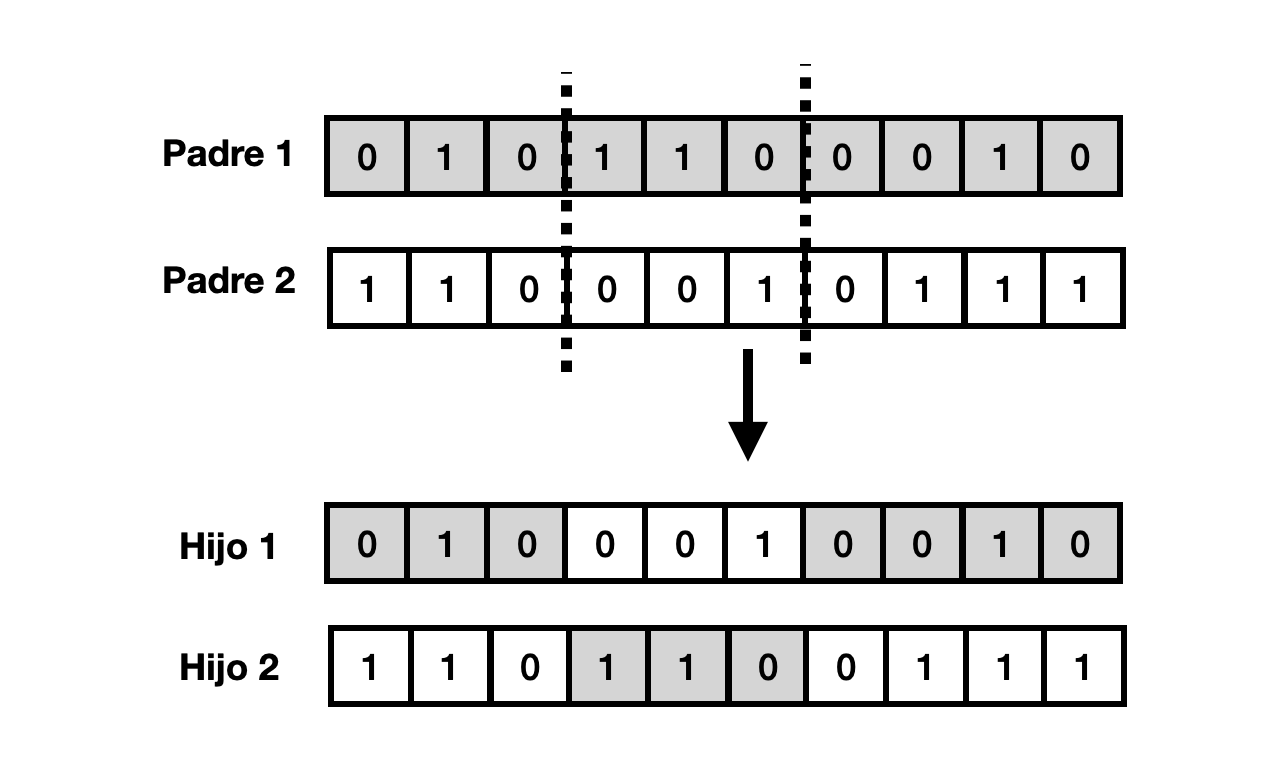
\includegraphics[width=0.9\textwidth]{images/crossOver.png}
  \caption{Ejemplo de crossover de dos puntos con dos cromosomas.}
  \label{fig:crossover}
\end{figure}

\cacho{Nuevo:}
En nuestro algoritmo, utilizamos una tasa de cruzamiento de \( c_r = 0{,}50 \) (\emph{tasa de crossover}), 
lo cual implica que, en cada generación, aproximadamente el 50\,\% de los individuos seleccionados para reproducción serán cruzados entre sí.  
Dado que la evolución se aplica sobre el 60\% de la población total (ver Sección~\ref{sec:selection}, comunmente llamados \emph{offspringSize} en los algortimos geneticos), esto equivale al:

\begin{equation}
\text{individuos\_cruzados} = r_c \cdot \text{offspringSize} = 0,50 \cdot \left(0,60 \cdot N\right)
\end{equation}

donde \( N \) representa el tamaño total de la población.  
Por ejemplo, si \( N = 50 \), entonces se generan \( 0{,}50 \cdot 30 = 15 \) individuos por cruzamiento.  
Los 15 individuos restantes se obtienen por mutación directa o copia de padres seleccionados, asegurando una mezcla equilibrada entre exploración y explotación en el espacio de soluciones.
\cacho{hasta aca}

\subsubsection{Operadores Genéticos: Mutación}

La mutación es un operador fundamental en los algoritmos genéticos, encargado de introducir cambios aleatorios en los cromosomas para aumentar la diversidad en la población.  
Cada bit del cromosoma tiene una pequeña probabilidad de ser modificado, lo que en una representación binaria implica invertir su valor ('0' a '1' o viceversa).  
Este mecanismo, denominado \emph{mutación por inversión de bits}, es especialmente adecuado para representaciones binarias como la utilizada en nuestro enfoque. 

\cacho{
En representaciones binarias, como la que usamos, se aplica la \emph{mutación por inversión de bits}.  
Cada bit tiene una probabilidad $m_P$ de cambiar su valor (de ‘0’ a ‘1’ o viceversa).  
La Figura~\ref{fig:mutation} muestra un ejemplo donde se modifican los bits en las posiciones 1, 4, 5 y 7.
La probabilidad $m_P$ suele mantenerse baja para evitar alteraciones drásticas que perjudiquen la convergencia.  
En nuestro caso, usamos $m_P = 0{,}05$, lo que significa que cada bit tiene un 5\% de probabilidad de mutar.
Este valor fue determinado experimentalmente para equilibrar la exploración y la preservación de soluciones prometedoras.
}
\cacho{Esto es nuevo tamb:}
Como los individuos están representados por cromosomas binarios de longitud $L$ y la población tiene tamaño $N$,  
la cantidad esperada de bits mutados por generación, $\mu$, se calcula como:

\[
\mu = N \cdot L \cdot P_m
\]

Donde $N$ es el tamaño de la población, $L$ es la longitud del cromosoma y $P_m$ es la probabilidad de mutación.
En nuestro caso, para la clase NCL, $N = 50$, $L = 20$ y $P_m = 0,05$, por lo que $\mu = 50 \cdot 20 \cdot 0,05 = 50$.
Esto indica que, en promedio, se mutan 50 bits de toda la poblacion por generación

Para nuestro caso concreto, como ya explicamos, cada posición del cromosoma representa un método específico de la API, entonces una mutación en la posición 3 implicaría activar o desactivar el método
correspondiente en el individuo, de acuerdo a la tabla \ref{tab:ncl-api-infer}, seria el método \emph{add(Object)}.
Este tipo de variaciones permite explorar diferentes combinaciones de subconjuntos de métodos que de otra manera no se generarían.  

\begin{figure}
    \centering
    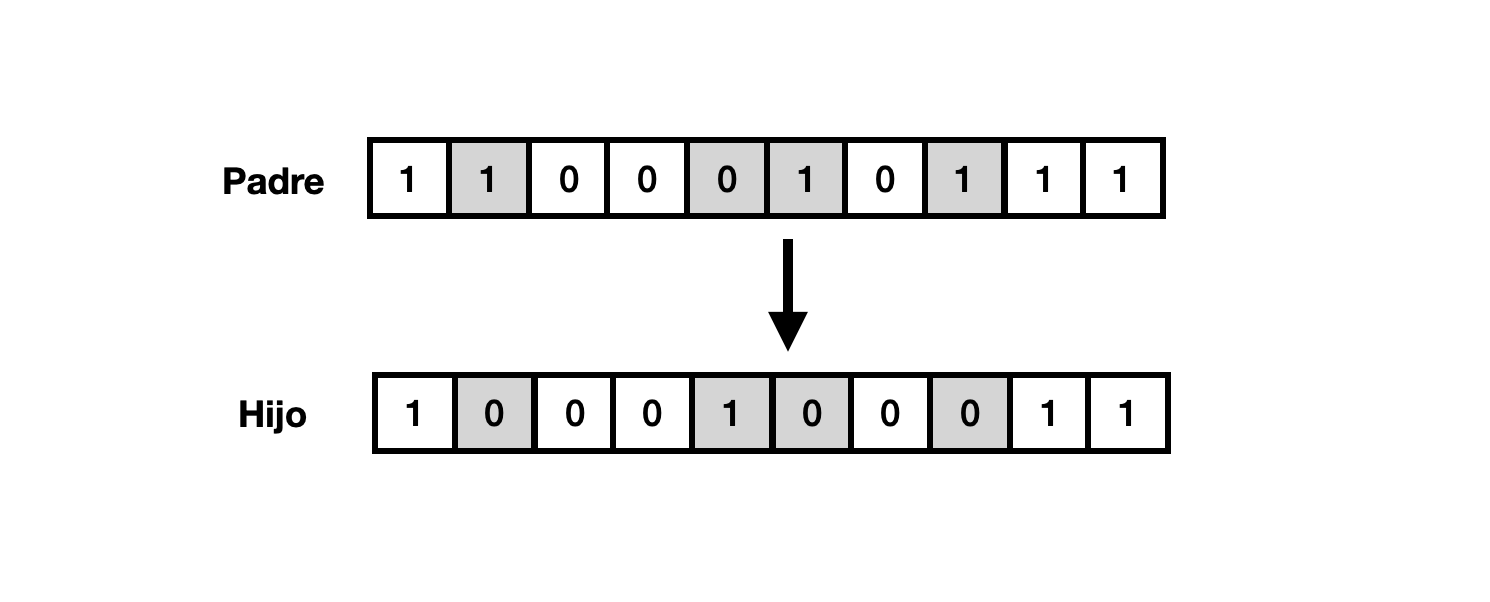
\includegraphics[width=0.9\textwidth]{images/mutation.png}
    \caption{Ejemplo de mutación por inversión de bits.}
    \label{fig:mutation}
    \end{figure}
\subsubsection{Pseudocódigo del algoritmo genético}

El algoritmo~\ref{alg:enfoqueGA} muestra un pseudocódigo del algoritmo genético que definimos para la búsqueda de métodos generadores de objetos.

\cacho{TODO ESTO ES NUEVO:}

\begin{algorithm}
  \caption{Algoritmo genético para la identificación de métodos generadores de
  objetos}
  \label{alg:enfoqueGA}
  \begin{algorithmic}[1]
  \STATE $pop \gets$ generar población de cromosomas con un solo gen en true
  \STATE $offspringSize \gets 0.6 \times N$
  \STATE $survivorSize \gets N - offspringSize$
  \FOR{$i \gets 0$ \TO $numEvo$}
      \STATE $survivors \gets$ seleccionar $survivorSize$ por torneo de tamaño $tournamentSize$ de $pop$
      \STATE $offspring \gets$ \{\}
      \FOR{$j \gets 1$ \TO $offspringSize$}
          \STATE $c_1 \gets$ torneo($pop$, $tournamentSize$, $f(s)$)
          \STATE $c_2 \gets$ torneo($pop$, $tournamentSize$, $f(s)$)
          \IF{$rand() < crossoverRate$}
            \STATE $child \gets$ dosPuntosCrossover($c_1$, $c_2$)
          \ELSE
            \STATE $child \gets$ más apto entre $c_1$, $c_2$
          \ENDIF
          \STATE añadir $child$ a $offspring$
      \ENDFOR
      \FORALL{$c \in offspring$}
          \STATE $new \gets$ mutar($c$, $mutacionRate$)
          \IF{$new \ne c$}
            \STATE remplazar $c$ por $new$ en $offspring$
          \ENDIF
      \ENDFOR
    \STATE $pop \gets survivors \cup offspring$
    \STATE $C \gets$ mejor cromosoma de $pop$
    \IF{aptitud de $C$ es constante durante $maxIter$}
        \STATE detener algoritmo
    \ENDIF
  \ENDFOR
\STATE $result \gets$ $C$


\end{algorithmic}
\end{algorithm}


% \begin{algorithm}
%   \caption{Algoritmo genético para la identificación de métodos generadores de
%   objetos}
%   \label{alg:enfoqueGA}
%   \begin{algorithmic}[1]
  
%   \STATE $P \gets$ generar población aleatoria
%   \FOR{$i \gets 0$ \TO $numEvoluciones$}
%       \STATE $P \gets$ $popSize$ cromosomas más aptos de $P$
%       \FOR{$j \gets 1$ \TO $\text{tasaC} \times |P|$}
%           \STATE $C_1, C_2 \gets$ dos cromosomas más aptos 
%           \STATE cruzar($C_1, C_2$)
%       \ENDFOR
%       \FORALL{cromosomas en $P$}
%           \STATE mutar $1/\text{tasaMutacion}$ genes
%       \ENDFOR
  
%     \STATE $C \gets$ mejor cromosoma de $P$
%     \STATE $actual \gets$ estado inicial

%     \IF{aptitud de $C$ es constante durante $maxIter$}
%         \STATE detener algoritmo
%     \ENDIF
% \ENDFOR

% \end{algorithmic}
% \end{algorithm}

Los elementos descritos a continuación corresponden a las partes constitutivas del algoritmo genético implementado en nuestro enfoque 
para identificar subconjuntos de métodos generadores. 
El algoritmo~\ref{alg:enfoqueGA} sigue la estructura típica de un algoritmo evolutivo, adaptado específicamente a nuestro problema.

La población inicial se construye en la línea 1, generando cromosomas válidos, donde cada uno representa un subconjunto de métodos con exactamente un método activo.
Esta decisión inicial asegura diversidad mínima, permitiendo explorar combinaciones desde los métodos más simples hacia conjuntos más complejos 
a lo largo de la evolución.

En la línea 2 y 3 se define el tamaño de la poblacion que va a ser la descendencia, la misma es definida como un 60\% del tamaño de la poblacion total $N$, 
y el resto (40\%) se mantiene como sobrevivientes de la población actual. A partir de allí, el algoritmo entra en el bucle evolutivo que se repite durante un número máximo de generaciones $numEvo$ (línea 4).


En cada iteración, se seleccionan los individuos sobrevivientes mediante un proceso de \textit{selección por torneo} (línea 5), utilizando el parámetro $tournamentSize$ como tamaño de torneo.
A continuación, se genera una descendencia en la línea 6 a través de un ciclo de reproducción que recorre $offspringSize$ veces.

Cada nuevo individuo se genera a partir de dos padres seleccionados también mediante torneo (líneas 7-8). 
Con una probabilidad $crossoverRate$, se aplica un operador de \textit{cruzamiento de dos puntos} (línea 11); en caso contrario, se elige el más apto entre los dos padres (línea 13).
Luego de generada la descendencia, se aplica el operador de \textit{mutación} (líneas 17-22) sobre cada individuo. 
La mutación se realiza gen a gen con una probabilidad $mutationRate$, y si el cromosoma mutado es diferente del original, se reemplaza.

La nueva población para la siguiente generación se construye uniendo los sobrevivientes y la descendencia (línea 23). A partir de esta población, se determina el mejor cromosoma actual (línea 24).
El algoritmo verifica si la aptitud del mejor cromosoma se mantiene constante durante un número de generaciones consecutivas igual a $maxIter$ (líneas 25 a 27). Si esto ocurre, se detiene anticipadamente.

La función objetivo utilizada durante todo el proceso es la definida en la sección~\ref{sec:fitnessGE}, y tiene en cuenta tres componentes: cantidad de objetos generados, minimalidad (métodos usados) y complejidad de parámetros. 
Esta función se utiliza tanto en los torneos como para evaluar los resultados de cruce y mutación.

Finalmente, el mejor cromosoma encontrado se retorna como resultado del algoritmo (línea 29).

Todos los parámetros del algoritmo fueron definidos de manera experimental.
Los valores utilizados en nuestras evaluaciones son: tamaño de población $N = 50$, tasa de cruzamiento $crossoverRate = 0.50$, tasa de mutación $mutationRate = 0.05$, número máximo de generaciones $numEvo = 20$ y iteraciones máximas $maxIter = 5$.
 
Existe un compromiso al elegir un buen valor para $numEvo$: un número mayor aumenta la precisión del algoritmo pero incrementa su tiempo de ejecución, 
mientras que un número menor lo hace más rápido pero podría no encontrar el
mejor conjunto de generadores de objetos.

Para implementar el algoritmo genético, utilizamos una biblioteca muy popular en Java llamada \emph{Jenetics}\footnote{\url{https://jenetics.io/}}, versión 5.2.0 \cacho{Esto en experimental?}. Esta biblioteca está diseñada específicamente para algoritmos evolutivos y nos proporcionó las herramientas necesarias para desarrollar nuestro enfoque genético.
\emph{Jenetics} es una biblioteca robusta y versátil que ofrece una amplia gama de funcionalidades para la implementación de algoritmos genéticos. Nos permitió definir y manipular genes, cromosomas y poblaciones, así como utilizar operadores genéticos como selección, cruzamiento y mutación. Además, cuenta con un sólido conjunto de herramientas de optimización y técnicas de evolución que nos permitieron adaptar el algoritmo a nuestras necesidades específicas.
Gracias a \emph{Jenetics}, pudimos implementar el algoritmo genético de manera eficiente y efectiva, lo que nos permitió explorar y encontrar subconjuntos óptimos de métodos \emph{builders} para las diferentes estructuras de datos en nuestro estudio. Además, \emph{Jenetics} es muy fácil de usar, con una documentación completa y una comunidad activa de usuarios que proporciona soporte y ayuda.
Una característica relevante de \emph{Jenetics} es que permite realizar la evaluación de los individuos de la población en paralelo utilizando el \emph{ForkJoinPool.commonPool()}, lo que mejora notablemente el rendimiento en sistemas con múltiples núcleos. Esta paralelización se gestiona de forma transparente, sin necesidad de implementar hilos manualmente, y puede personalizarse en caso de requerirse un control más detallado del entorno de ejecución.
\cacho{HASTA ACA}


\subsection{Algortimo de Escalada de Colinas}
\label{alg:approachHC}

El segundo algoritmo, denominado en inglés \textit{hill climbing},
\cite{Russell:2009, Cormen2009, kleinberg2006}, es un algoritmo de búsqueda local basado en la escalada de colinas.
Es un algoritmo greedy que selecciona en cada paso el estado vecino con mayor
valor en la función objetivo. 
Así, el algoritmo de escalada de colinas parte de un estado inicial y lo mejora sucesivamente hasta alcanzar un estado que no puede ser mejorado (estado pico). 
Para guiar este proceso se emplea una función heurística que evalúa la calidad de cada estado.
Por sus características, el algoritmo de escalada de colinas suele encontrar soluciones
con rapidez. Sin embargo, puede quedarse atrapado en óptimos locales donde
ningún vecino inmediato es mejor, pero existen mejores soluciones en el espacio
de búsqueda. Esto es, el algoritmo no siempre encuentra una solución óptima.

Su principal diferencia con los algoritmos genéticos radica en el mecanismo de selección. Mientras que en la escalada de colinas se generan y evalúan todos los vecinos del estado actual seleccionando el óptimo inmediato, 
los algoritmos genéticos operan mediante recombinación y mutación de una población de soluciones. 
En nuestra implementación, tanto los candidatos como la función objetivo son idénticos para ambos algoritmos.


\pp{El algoritmo debería ir en un float también porque sino quedan mal los espacios.}

\SetKwFunction{Compute}{Compute} 
\SetKwFunction{fBuilders}{computeBuilders}
\SetKwFunction{hc}{hillClimbing}
\SetKwFunction{successor}{generarSucesores}
\SetKwFunction{mejorSuccesor}{mejorSuccesor}
\SetKwFunction{generarSucesores}{generarSucesores}
\SetKwFunction{isCons}{esConstructor}

\SetKwProg{Fn}{Function}{:}{}

\begin{algorithm}[H]
    \caption{Algoritmo hill-climbing para la identificación de métodos
    generadores de objetos}
    \label{alg:enfoqueHC}

    \Fn{\fBuilders{}}{
        $initial \gets [0,0,\ldots,0]$\;
        $cons \gets$ \hc{initial, true}\;
        \Return \hc{cons, false}\;
    }
    \BlankLine

    \Fn{\hc{$initialState, const$}}{
        $curr \gets initialState$\;
        \While{true}{
            $successors \gets$ \successor{$curr$, const}\;
            $best \gets$ \mejorSuccesor{$successors$}\;
            \If{$f(best) \leq f(curr)$}{
                \Return $curr$\;
            }
            \Else{
                $curr \gets best$\;
            }
        }
    }
    \BlankLine

    \Fn{\successor{$state$, $const$}}{
        $initial \gets []$\;
        \For{$i \gets 0$ \KwTo \#M}{
            \If{$s[i] == 0$}{
                \pp{qué es builders? No se entiende la condición}\;
                \If{($const$ \textbf{and} $isConstructor(i)$) || (!$const$ \textbf{and} !$isConstructor(i)$)}{
                    $successor \gets clone(s)$\;
                    $successor[i] \gets 1$\;
                    $successors.add(successor)$\;
                }
            }
        }

        \Return $successors$\;
    }
    \BlankLine

    \Fn{\mejorSuccesor{$successors$}}{
        $curr \gets -INF$\;
        \For{$i \gets 0$ \KwTo \#successors}{
            \If{$s[i] > bestVal$}{
                $bestVal \gets f(s[i])$\;
                $best \gets s[i]$\;
            }
        }
        \Return $best$\;
    }


\end{algorithm}

El algoritmo~\ref{alg:enfoqueHC} muestra el pseudocódigo de nuestro enfoque basado en un algoritmo de escalada de colinas para la identificación de métodos generadores de objetos . 
La representación que hemos utilizado del problema es la explicada en la sección
\ref{sec:estados}. Esto quiere decir que utilizamos vectores de bits para
representar los estados. \pp{Y las funciones objetivo?}
El proceso comienza con la función principal $computeBuilders$, que implementa
la búsqueda. 
La inicialización consiste en definir un estado inicial representado por un vector de ceros, 
que indica que ningún método está seleccionado. Este estado se pasa como parámetro a la función $hillClimbing$, junto con un valor lógico que indica que se deben considerar únicamente los métodos constructores. 
Posteriormente, el algoritmo invoca nuevamente a $hillClimbing$ para continuar la búsqueda incluyendo los otros métodos de la API con el mejor constructor que obtuvo
la busqueda anterior (línea 1 a 5).

La función $hillClimbing$ constituye el núcleo del algoritmo de Hill Climbing. Su ejecución parte del estado inicial recibido por parámetro y, 
mediante un ciclo iterativo, genera todos los posibles sucesores del estado actual utilizando la función $generarSuccessor$. 
Entre estos sucesores se selecciona el que presente el mejor valor según la función de fitness $f$. Si dicho sucesor no mejora el valor del estado actual,
el algoritmo concluye devolviendo el estado alcanzado. En caso contrario, el mejor sucesor pasa a ser el nuevo estado y el ciclo continúa. (línea 6 a 17)

La generación de sucesores se realiza en la función $generarSucesores$. Esta función evalúa cada posición del vector de estado. Si una posición tiene el valor 0 
(indicando que el método correspondiente no está seleccionado) se evalúa si puede activarse en función de si se está buscando metodos constructores de la API o no. 
En caso de cumplir con esta condición, se genera un clon del estado actual en el que se activa dicha posición, y este nuevo estado se añade a la lista de sucesores. (línea 18 a 29). Ver figura \ref{fig:succ-hillClimbing}

\begin{figure}[H]
    \centering
    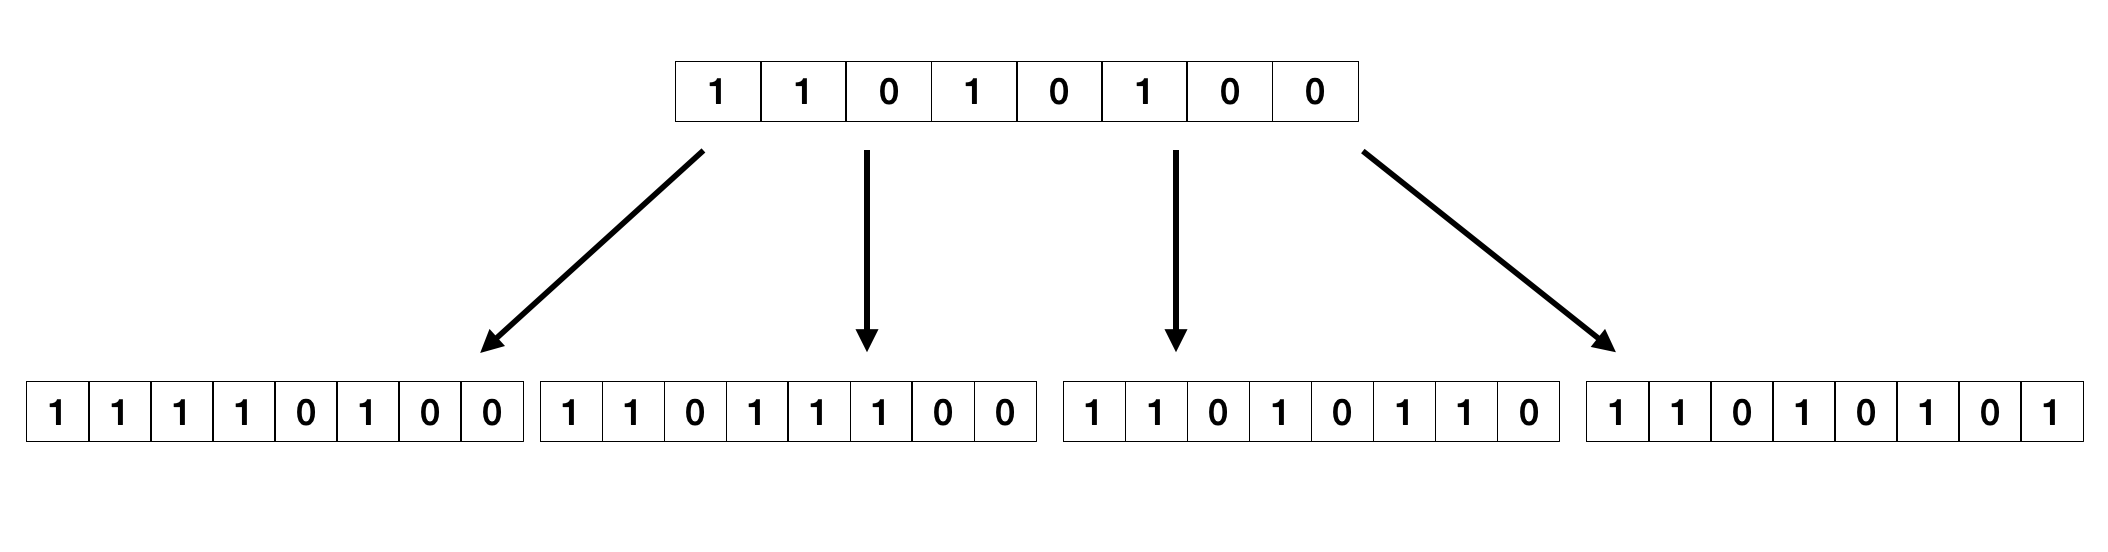
\includegraphics[width=0.95\textwidth]{images/succesores.png}
    \caption{Sucesores de un estado.}
    \label{fig:succ-hillClimbing}
  \end{figure}
  
Finalmente, la función $mejorSuccesor$ se encarga de seleccionar el mejor sucesor de la lista proporcionada.
Para ello, recorre la lista evaluando el valor de la función objetivo $f$ en
cada sucesor y selecciona aquel que tenga el mayor valor (líneas 30 a 38).


%Este enfoque de Hill Climbing presenta la ventaja de tener menos parámetros de configuración que los algoritmos genéticos, 
%lo que simplifica su implementación. Sin embargo, este tipo de búsqueda local implica el riesgo de quedar atrapado en óptimos locales, 
%dado que el algoritmo solo avanza hacia soluciones que mejoran directamente el estado actual. 
%
%En cualquier caso, el enfoque propuesto resulta eficiente en contextos donde se requiere una búsqueda controlada y directa, 
%sin la necesidad de manejar múltiples parámetros adicionales.
%


% En cada iteración, \emph{Hill Climbing} generar los sucesores del estado corriente (Línea 5). Esto se puede observar en el algoritmo \ref{alg:sucessores}. 
% Esto, simplemente, genera estados sucesores prendiendo únicamente un bit (poniendo 1) por cada bit apagado (bit en 0). 
% Esto significa que crear un sucesor para nuestro problema es agregar un método al estado corriente. El método \emph{generarSucesores} nos devuelve el conjunto de estados del estado \emph{curr}. \pp{Esto también está desordenado. Habría que poner un ejemplo con figuras para que se entienda bien qué hace.}

% El método que genera los sucesores nos devuelve un conjunto de posibles soluciones que se crean a partir de sumarle un método a la solución óptima corriente ($curr$). Es decir, los sucesores  $S$ generados con \emph{GenerarSucesores(curr)} de un candidato $curr$ son los conjuntos {$curr\cup{mi}$}, para cada $mi$ $\in$ API (Línea 3) \pp{Se podría poner el pseudocódigo de generar sucesores, y quizás poner un ejemplo para que se entienda}.
% Sea $best$ el sucesor con valor objetivo más alto (línea 6), si este tiene un valor que es menor o igual al corriente, significa que no hay un sucesor mejor y el algoritmo retorna el estado corriente (Línea 7 y 8). Se puede observar que este estado es un máximo local y el algoritmo lo encontró.
% En caso de que el valor del estado corriente sea menor al mejor sucesor encontrado en la iteración, se reemplaza el corriente y vuelve a ejecutar una nueva iteración con este estado hasta encontrar un máximo local. \pp{Esto también está explicado arriba, y ahora de nuevo. Hay que ordenarlo.}
% Observe que $best$ tiene exactamente un método más que el mejor candidato de la iteración anterior, $curr$ (Línea 4) \pp{hay que implementar con código el existe un mejor candidato. Mirar el libro de AI.}.

%Se puede observar que este algoritmo puede quedar atrapado en un máximo local y no generar alguna combinación específica que podría ser aún mejor. Aquí se puede ver que es un algoritmo perezoso, ya que obtiene una solución rápida, pero puede no ser eficaz en encontrar la mejor solución global. 

%\subsubsection{Clases de equivalencia}
%\label{alg:approachCE}
 %Las clases de equivalencia son una técnica utilizada para agrupar conjuntos de datos de entrada en categorías o clases que tienen un comportamiento similar o producen resultados equivalentes. Esta técnica es ampliamente utilizada en el diseño y la realización de pruebas de software.
 %En términos generales, una clase de equivalencia representa  un conjunto de que se espera que produzcan resultados idénticos. La idea es que si un conjunto de la clase de equivalencia produce un resultado, entonces todas las demás entradas de esa clase deberían producir el mismo resultado.
 %Al trabajar con clases de equivalencia, se selecciona una entrada representativa, llamada caso de prueba, de cada clase para ser evaluada. En lugar de probar todas las posibles entradas, se eligen casos de prueba que representen cada clase de equivalencia para minimizar la cantidad total de pruebas necesarias.

 %Bajo esta introducción, hemos desarrollado un tercer algoritmo donde agrupamos en clases de equivalencia aquellos subconjuntos de métodos que tengan el mismo valor de la función objetivo con alguna de las funciones explicadas en \ref{sec:fitness}.

%\subsection{Pseudo-Código}

%\begin{figure}[H]
%\begin{lstlisting}[style=javaStyle, caption={Algoritmo basado en Clases de Equivalencia}, label={algo:clases_equivalencia}]
%public Estado clasesDeEquivalencia() {
%    Estado curr = generarEstadoIncial(problem,funObjectivo);
%    Map<Key, Estado> equivalenceClasses = crearClasesDeEquivalencia(curr);

%    boolean newClassCreated;
%    do {
%        newClassCreated = false;
%        Set<Estados> newCandidates = candidatosPorClase(equivalenceClasses);

%        for (Estado candidate : newCandidates) {
%            Queue<Estado> successors = generarSucesores(candidate);
%            for (Estado successor : successors) {
%                Double key = successor.value;
%                equivalenceClasses.get(key).add(successor);
%                newClassCreated = true;
%            }
%        }
%    } while (newClassCreated);

%    Set<Estado> best = obtenerMejor(equivalenceClasses);
%    return best;
%}
%\end{lstlisting}
%\end{figure}


%En este algoritmo, se comienza obteniendo los conjuntos \emph{singletons} (Línea 1), que son los métodos constructores individuales de la misma manera que el algoritmo de \ref{alg:hill_climbing}. Esto es nuestro estado inicial del algoritmo. A partir de estos singletons, se crea una clase de equivalencia con la \emph{key} que es la función de valoración de cada estado inicial y se agrupan los estados que tienen el mismo valor de valoración. Esto servirá como punto de partida de nuestro algoritmo. (Línea 3).  En el algoritmo las clases de equivalencias están guardadas en $equivalenceClasses$.

%Luego comienza la etapa iterativa (Línea 6 a 18) mientras se haya creado una nueva clase de equivalencia. En cada iteración, se generan nuevos candidatos por cada clase de equivalencia. Es decir, se selecciona un candidato de cada clase de equivalencia (el que tenga menor cantidad de métodos y menor cantidad de parámetros) $candidatosPorClase(equivalenceClasses)$ y se lo guarda en una cola ($newCandidates$) (Línea 8). A continuación, se generan los sucesores (línea 10 y 11) para cada candidato elegido, $GenerarSucesores(candidate)$, utilizando el mismo enfoque que en el algoritmo \ref{alg:sucessores}. Estos se guardan en $successors$. Es decir, si tenemos $N$ clases de equivalencias vamos a tener $N$ candidatos a los cuales le vamos a calcular sus sucesores.  Luego, por cada uno de estos sucesores se le calcula su función de valoración y de acuerdo a esta se lo guarda en la clase de equivalencia representada por el valor de valoración (Línea 14).
%El algoritmo itera hasta que no hayamos creado una nueva clase de equivalencia. Si no hemos creado una clase de equivalencia nueva, quiere decir que no hay cambios y hemos explorado todas las alternativas posibles. 

%Luego, para obtener el mejor conjunto de métodos generadores de objetos que estamos buscando, accedemos a la clase de equivalencia que tenga la \emph{key} más grande (mejor función de valoración) y obteniendo el representante de ese conjunto que tenga menor método y parámetros. Esto lo realiza el método $obtenerMejor(equivalenceClasses)$



% En la búsqueda de soluciones óptimas mediante algoritmos genéticos u otros algoritmos de búsqueda, la función de valoración \cite{goldberg1989genetic} desempeña un papel fundamental. Su diseño adecuado es crucial, ya que determina la dirección y el éxito del proceso de búsqueda.
% La función de valoración evalúa la calidad de cada solución candidata y la compara con otras soluciones en la población. Proporciona una medida objetiva de la idoneidad de cada individuo en relación con los objetivos y restricciones del problema. La calidad se expresa generalmente mediante un valor numérico, donde valores más altos indican soluciones más deseables. Por ejemplo, si estamos resolviendo un problema de optimización en el que buscamos maximizar una función objetivo, la función de valoración puede asignar un valor más alto a las soluciones que se acercan más a la solución óptima. Por otro lado, si estamos resolviendo un problema de minimización, la función de valoración puede asignar un valor más alto a las soluciones que se alejan más de la solución óptima.
% Definir una buena función de valoración implica considerar cuidadosamente los requisitos y características del problema en cuestión. Puede implicar ponderar diferentes objetivos, como maximizar o minimizar ciertas variables, satisfacer restricciones específicas o lograr un equilibrio entre múltiples criterios. 

% Una función de valoración efectiva debe ser capaz de discriminar entre soluciones prometedoras y soluciones subóptimas. Debe proporcionar una evaluación objetiva y precisa, permitiendo la selección de soluciones de alta calidad y la eliminación de soluciones menos deseables.
% Además, la función de valoración debe ser adecuada para el dominio y el tipo de problema abordado. Puede requerir conocimiento especializado y experiencia en el campo para definir correctamente las métricas y ponderaciones apropiadas. 

% Es importante tener en cuenta que la función de valoración puede evolucionar y adaptarse a lo largo del proceso de búsqueda. A medida que el algoritmo de busqueda avanza y produce nuevas generaciones de soluciones, la función de valoración puede ser ajustada y refinada para enfocarse en las características más relevantes y deseadas.


% Por lo tanto, en los algoritmos de búsqueda la función de valoración desempeña un papel crucial para evaluar y comparar soluciones candidatas en función de criterios específicos del problema. Proporciona una medida cuantitativa de la calidad de las soluciones y guía el proceso de selección y toma de decisiones en cada etapa del algoritmo. El diseño adecuado de la función de valoración es esencial para obtener resultados óptimos y eficientes en la resolución de problemas.
% A continuación, explicaremos cada función de valoración implementada en nuestros algoritmos.


% En el caso de algoritmos greedy, la función de valoración juega un papel similar pero con un enfoque más local. En lugar de trabajar con una población de soluciones, los algoritmos greedy toman decisiones en cada paso basándose en una evaluación local de las opciones disponibles. La función de valoración en un algoritmo greedy se utiliza para seleccionar la mejor opción en cada iteración o paso del algoritmo, maximizando o minimizando la función de valoración según el objetivo del problema \cite{cormen2009introduction}.





\chapter{Generacion Exhaustiva acotada desde API de los programas}


\label{cap:beapi}

En adelante, se presenta la técnica desarrollada llamada BEAPI, que tiene como objetivo mejorar la generación exhaustiva acotada (BEG, por sus siglas en inglés, \emph{Bounded Exhaustive Generation}). \ref{sec:BE}. \cacho{Agregar en preliminar? ampliar?}
La generación exhaustiva acotada se refiere a un enfoque en pruebas de software y análisis de sistemas en el cual se generan y evalúan todas las posibles combinaciones o instancias de entrada dentro de un conjunto acotado. Esto significa que se examinan todas las combinaciones posibles de entrada dentro de un límite especificado. Es un enfoque efectivo para revelar fallas en el sofware. Este enfoque se utiliza a menudo en sistemas donde el espacio de entrada es manejable y finito. 
Existen varios enfoques de BEG que requieren una especificación precisa de que entradas son válidas en el contexto del sistema. Esta especificación comúnmente se llaman \emph{RepOK} y debe ser brindada por el usuario.
En este capítulo, introduciremos BEAPI, un enfoque eficiente que genera un conjunto exhaustivo acotado de objetos realizando únicamente llamadas a la API de un módulo. Discutiremos las principales ideas de nuestros enfoques para generar de manera eficiente. Este capítulo está organizado de la siguiente manera: en la Sección \ref{sec:motivating-example}, se presenta un ejemplo que ilustra el problema que se aborda con la técnica propuesta, la cual se explica en la Sección \ref{sec:beapiIntro}. Luego, en las Secciones \ref{sec:scope}, \ref{sec:stateMatching} y \ref{sec:builders}, se describen las optimizaciones implementadas en BEAPI. Estas optimizaciones son de vital importancia a la hora de trabajar con BE, ya que necesitamos acortar el espacio de búsqueda para poder generar suites exhaustivas acotadas con un rendimiento comparable al de las técnicas basada en especificaciones, una de ellas es \emph{Korat}\cite{Boyapati02} 


\section[Motivación]{Motivación}
\label{sec:motivating-example}


\begin{figure}[!thb]
\begin{lstlisting}
public boolean repOK() {
  if (this.header == null) return false;
  //  Missing constraint: the value of the sentinel node
  // must be null  
  // if (this.header.value != null) return false;
  if (this.header.next == null) return false;
  if (this.header.previous == null) return false;
  if (this.cacheSize > this.maximumCacheSize) return false;
  if (this.size < 0) return false;
  int cyclicSize = 0;
  LinkedListNode n = this.header;
  do {
      cyclicSize++;
      if (n.previous == null) return false;
      if (n.previous.next != n) return false;
      if (n.next == null) return false;
      if (n.next.previous != n) return false;
      if (n != null) n = n.next;
  } while (n != this.header && n != null);
  if (n == null) return false;
  if (this.size != cyclicSize - 1) return false;
  int acyclicSize = 0;
  LinkedListNode m = this.firstCachedNode;
  Set visited = new HashSet();
  visited.add(this.firstCachedNode);
  while (m != null) {
      acyclicSize++;
      if (m.previous != null) return false;
      // Missing constraint: the value of cache nodes
      // must be null
      // if (m.value != null) return false;
      m = m.next;
      if (!visited.add(m)) return false;
  }
  if (this.cacheSize != acyclicSize) return false;
  return true;
}
\end{lstlisting}
\caption{\texttt{repOK} de \texttt{NodeCachingLinkedList} tomado del benchmarks de \textsf{ROOPS}}
\label{fig:NCL-repOK}
\end{figure}

Para motivar las dificultades de escribir especificaciones formales para la generación de exhaustiva acotada de  estructuras, considere el invariante de representación (comúnmente llamados \emph{repOK}) de la clase \emph{NodeCachingLinkedList} (NCL) de Apache, que se muestra en la Figura \ref{fig:NCL-repOK}. Este es un \emph{repOK} del \emph{benchmarks} \emph{ROOPS}. Los NCL se componen de una lista principal circular doblemente enlazada con un nodo ficticio al comienzo de la estructura. Esta estructura es utilizada para el almacenamiento de datos, y una caché de nodos previamente utilizados implementada como una lista enlazada simple. Los nodos eliminados de la lista principal se mueven a la caché, cambiando su valor a \emph{null}, donde se guardan para su uso en el futuro. De esta manera, cuando se requiere un nodo para una operación de inserción, se reutiliza un nodo de la caché (si existe) en lugar de asignar un nuevo nodo. El objetivo es evitar la sobrecarga de recolección de basura para las aplicaciones que realizan una gran cantidad de inserciones y eliminaciones en la lista. El \emph{repOK} devuelve true si y solo si la estructura de entrada satisface las propiedades estructurales de NCL \cite{Liskov00}. En la figura \ref{fig:nclInstanceRepOK} se pueden observar instancias válidas de la estructura.

\begin{figure}[H]
    \centering
    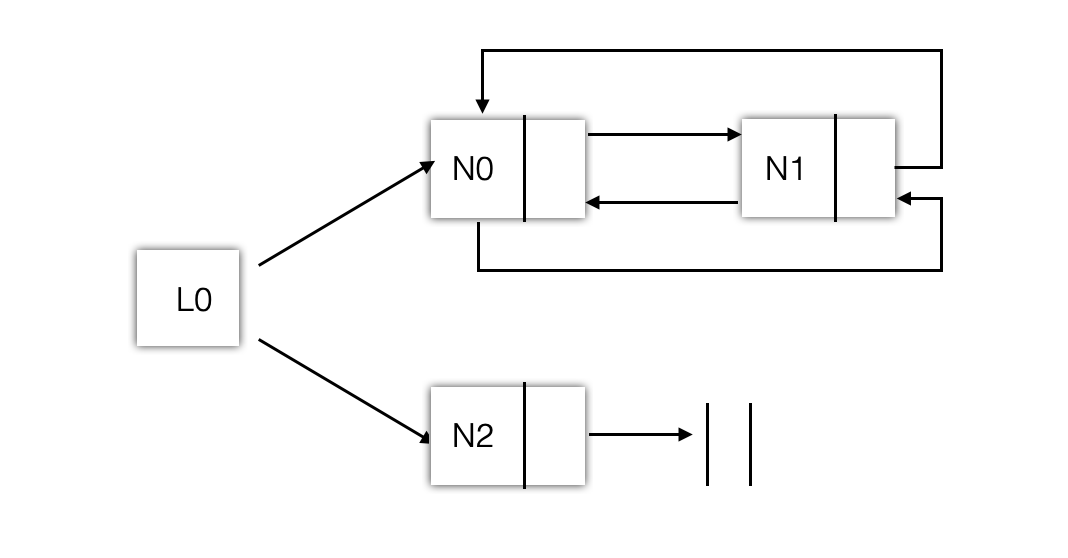
\includegraphics[width=0.85\textwidth]{NCL.jpg}
    \caption{Instancia de NodeCachingLinkedList}
    \label{fig:nclInstanceRepOK}
\end{figure}
Las restricciones impuestas en el método Java que abarca las líneas 2 a 11 se refiere a la verificación de la estructura general de \emph{Node Caching LinkedList}, como por ejemplo la existencia de un nodo ficticio en la lista principal. Este nodo ficticio es generalmente un nodo especial que no contiene datos reales (deberia contener \emph{null} como valor del nodo), pero se utiliza como una especie de marcador de inicio que simplifica la manipulación de la lista. La idea es que este nodo ficticio tiene un enlace que apunta al primer elemento real de la lista. Por ejemplo, la figura \ref{fig:repOK1} nos muestra dos instancias de NCL. La lista de la parte superior es la lista principal y la lista de la parte inferior es la representación de la lista caché.  En la figura, la instancia del lado derecho es válida, la del izquierdo es inválida debido a que no cumple la especificación de poseer un nodo ficticio. El \emph{repOK} en la línea 6 controla esta situación y lanza falso como respuesta el método.

\begin{figure}
  \centering
  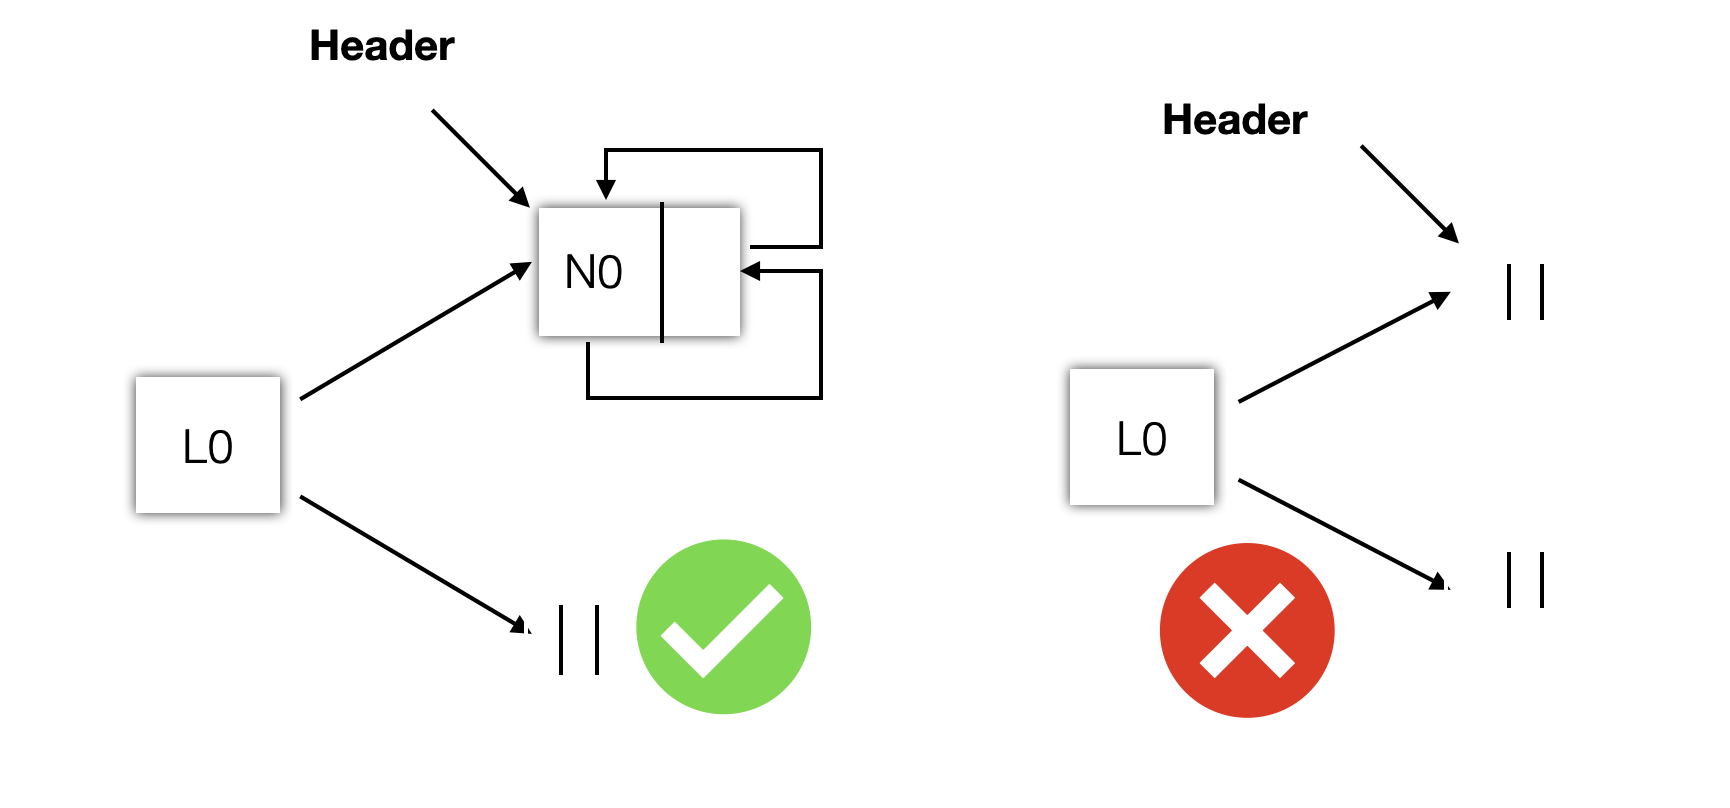
\includegraphics[width=0.8\textwidth]{images/repok1.jpg}
  \caption{Ejemplo una instancia válida y otra no de acuerdo al RepOK en las configuraciones generales de la estructura.}
  \label{fig:repOK1}
\end{figure}

Siguiendo con el análisis del \emph{repOK} de la figura \ref{fig:NCL-repOK}, las líneas 12 a 21 del método verifican que la lista principal sea una lista circular doblemente enlazada. Veamos en detalle lo que esto significa:
\cacho{Hace falta explciar la noción de lista ?}
\\
- Lista Circular: Una lista circular es aquella en la que el último elemento de la lista está enlazado al primer elemento, formando un ciclo. En otras palabras, si avanzamos a través de la lista desde el primer elemento, llegaremos eventualmente al último elemento y luego volveremos al primer elemento.
\\
- Doblemente Enlazada: En una lista doblemente enlazada, cada nodo tiene dos enlaces, uno que apunta al nodo anterior y otro que apunta al nodo siguiente. Esto permite recorrer la lista en ambas direcciones: desde el primer nodo hasta el último y viceversa.
\\
El método Java, que especifica la estructura entre las líneas 12 a 21, realizan un recorrido sobre la lista principal. 
En la figura \ref{fig:repok2} se puede observar ejemplos de instancia donde pasan o no esta sección de restricciones del método. La instancia de la izquierda muestra una lista principal correctamente construida, mientras que la instancia de la derecha tiene el error de  que la lista principal no es acíclica, característica que poseen las listas principales (donde se guardan los datos) de NCL. El campo \emph{next} del nodo \textbf{NO} apunta a \emph{null}, lo que rompe la propiedad de ciclicidad. Esta restricción se contempla en la linea 16 del \emph{repOK}.

\begin{figure}
  \centering
  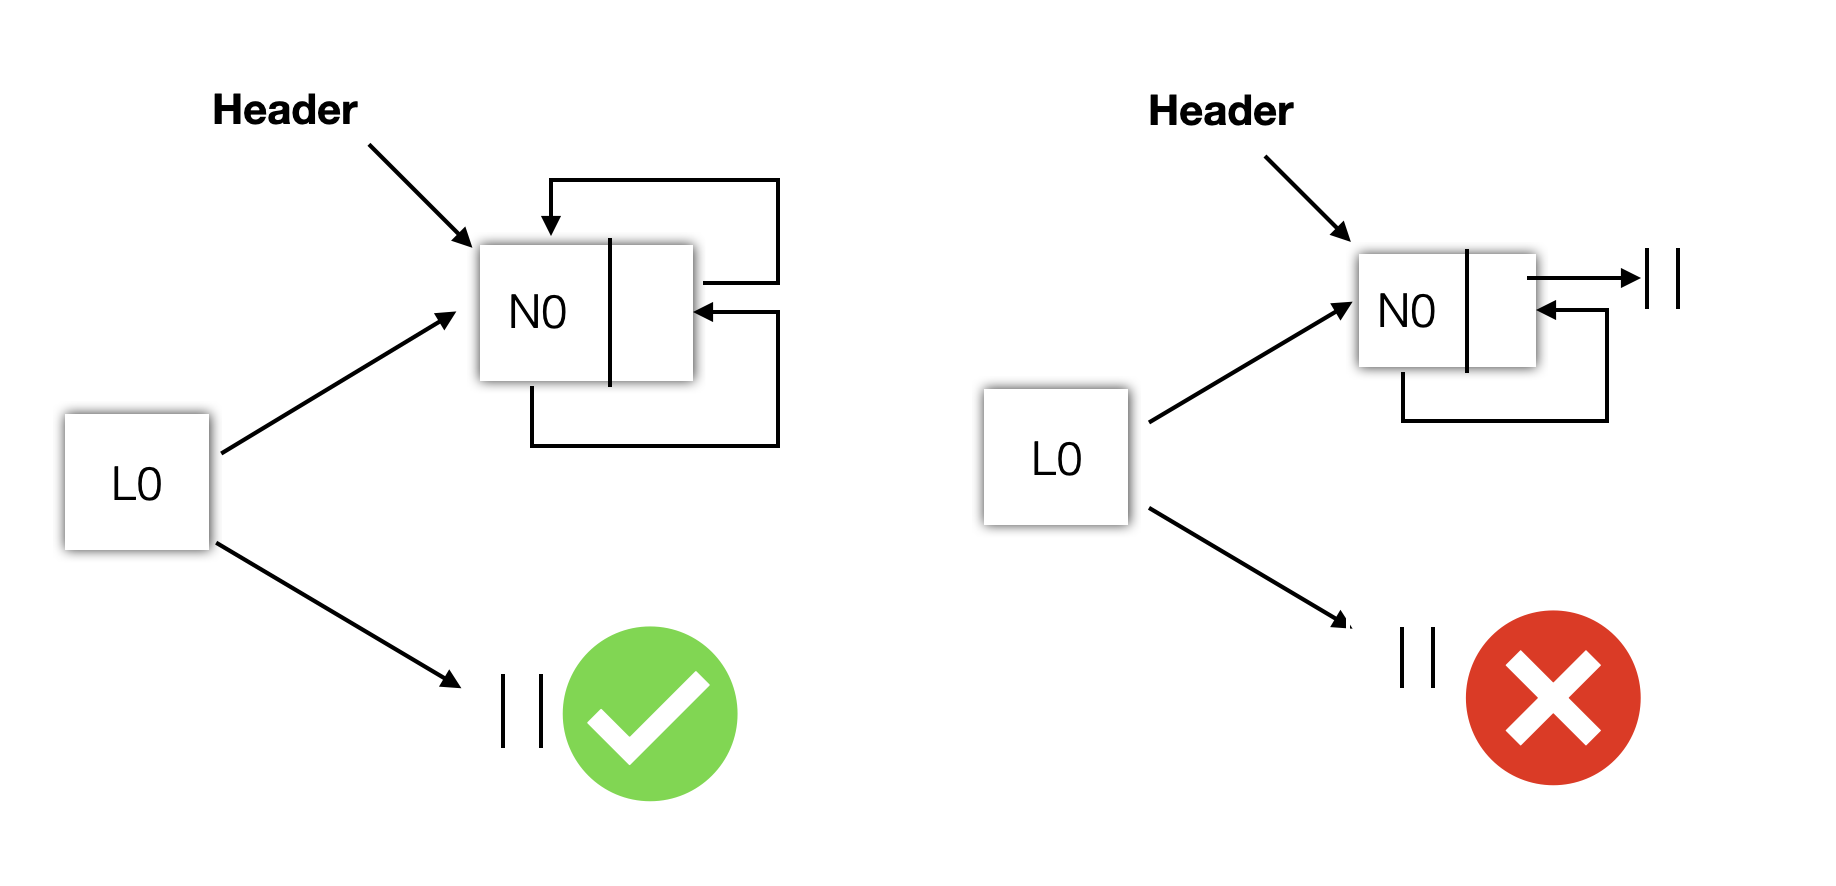
\includegraphics[width=1.1\textwidth]{images/repok2.jpg}
  \caption{Ejemplo una instancia válida y otra no de acuerdo al RepOK en la lista principal.}
  \label{fig:repok2}
\end{figure}

Por último, el método \emph{repOK} de la figura \ref{fig:NCL-repOK}, en las líneas 22 a 37 verifican que propiedades sobre la lista caché. Esta debe ser una lista simplemente enlazada terminada en un valor nulo (y se verifica la consistencia de los campos de tamaño en el proceso). Como ejemplo de esta situación, mostramos dos nuevas instancias en la figura \ref{fig:repok3}. La primera es una instancia válida de la lista caché y el \emph{repOK} nos devuelve True. La segunda instancia en la figura, nos muestra una instancia inválida de acuerdo a la especificación. Esto se debe a que la lista cache (la lista de la parte inferior de la estructura) es cíclica. La insatisfacción  de la propiedad se da cuando el método vuelve a insertar el mismo nodo al conjunto \emph{visited}. Este conjunto va recorriendo la lista y va chequeando en la línea 33 si vuelve a pasar por un nodo ya visitado. En caso de que esto suceda, retorna Falso. Esto es lo que sucede en la instancia de la figura \ref{fig:repok3}.

\begin{figure}
  \centering
  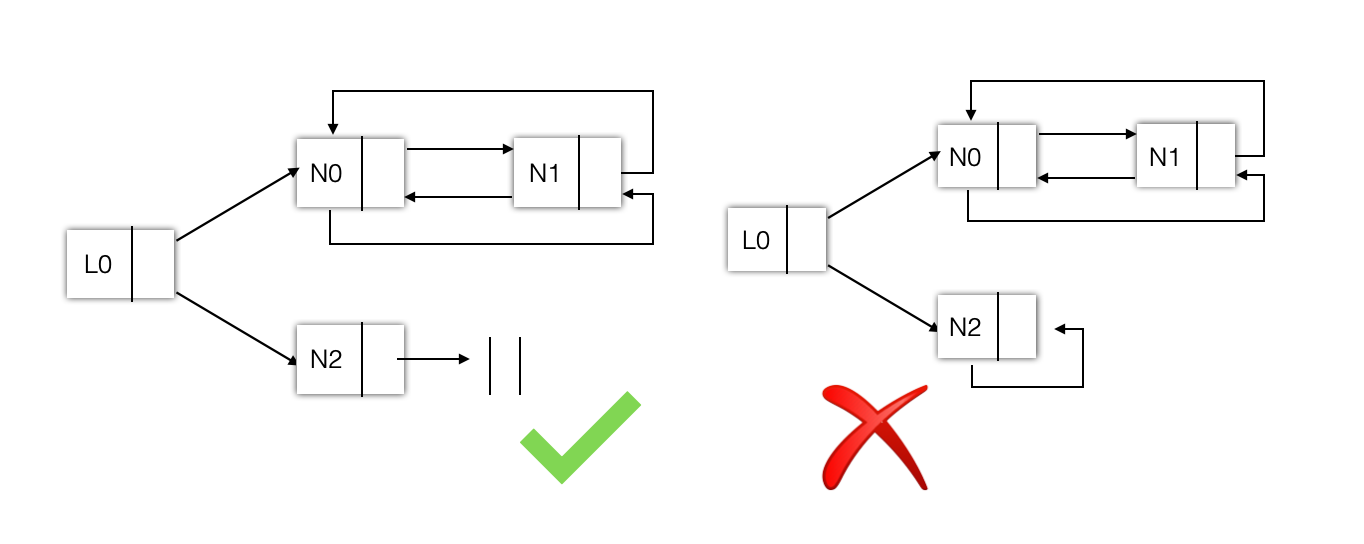
\includegraphics[scale=0.5]{images/repok3.jpg}
  \caption{Ejemplo una instancia válida y otra no de acuerdo al RepOK en la lista cache.}
  \label{fig:repok3}
\end{figure}

Este \emph{repOK} está escrito de la manera recomendada por los autores del enfoque de generación exhaustiva de BEAPI, \textsf{Korat} \cite{Boyapati02}.
Este método devuelve falso tan pronto como encuentra una violación de una propiedad prevista en la estructura actual. De lo contrario, devuelve verdadero al final de método. Esto permite a \textsf{Korat} podar grandes porciones del espacio de búsqueda ni bien se encuentra con alguna restricción que no se cumple, lo que mejora en gran medida su eficiencia.

En el \emph{repOK} de la figura \ref{fig:NCL-repOK}, se puede observar que existe código que está comentado y hace referencia a restricciones que faltan en el mismo. Estas restricciones no estaban presentes en el \emph{repOK} que tomamos de Roops; las agregamos después de analizar las estructuras generadas para las pruebas que resultaron incorrectas.

Olvidar alguna restricción provoca un aumento significativo en la cantidad de estructuras generadas, lo que complica la identificación de cuáles son válidas y cuáles no. Por ejemplo, el número de estructuras generadas por \emph{Korat} con el \emph{repOK}, sin las restricciones que están comentadas, asciende a 54.5 millones para un \emph{scope} de 8. Sin embargo, si agregamos las restricciones que faltan en el método de especificación, se generan solo 2.8 millones de estructuras para el mismo \emph{scope}. Esto podría llevarnos a generar varias estructuras como falsos positivos que luego seran utilizadas para realizar testing.

Motivados por estos problemas y la dificultad de escribir métodos \emph{repOK} para llevar a cabo la generación exhaustiva acotada, hemos desarrollado una técnica a la que denominamos BEAPI, la cual describiremos en las siguientes secciones.



\section[BEAPI]{BEAPI}
\label{sec:beapiIntro}

En esta sección discutimos las ideas principales de nuestros enfoques para generar de manera eficiente un conjunto exhaustivo acotado de objetos, haciendo solo llamadas a la API de un módulo. Nuestro enfoque se basan en la generación de pruebas dirigida por retroalimentación, explicado en la sección \ref{sec:feedback-directed-test-gen}.
El enfoque propuesto, denominado \textsf{BEAPI} (Bounded Exhaustive from API), introduce una técnica innovadora para la generación exhaustiva acotada. Este enfoque se basa en la realización de llamadas a los métodos de la API del software bajo prueba (SUT). Al igual que otros enfoques de generación de pruebas basados en API, \textsf{BEAPI} crea secuencias de llamadas a métodos de la API, conocidas como secuencias de test, y las ejecuta para generar estructuras. 

A diferencia de los enfoques de generación basados en caja negra, \textsf{BEAPI} no requiere una especificación formal de las propiedades de las estructuras. Al igual que otras técnicas de generación exhaustiva acotada (BEG), el usuario solo debe proporcionar los alcances para la generación, que se abordan en detalle en la sección correspondiente.  Esto permite generar estructuras válidas sin requerir una especificación detallada de las propiedades de las estructuras, reduciendo así la carga de trabajo para el programador.

La principal ventaja de \textsf{BEAPI} es que requiere un esfuerzo menor de especificación para realizar la generación exhaustiva acotada. Si los métodos de la API utilizados en la generación son correctos, todas las estructuras generadas serán válidas para su construcción. El programador solo necesita asegurarse de que los métodos de la API lancen excepciones cuando se violen las reglas de uso, siguiendo un estilo de programación defensivo \cite{Liskov00}. En la mayoría de los casos, esto implica verificar condiciones muy simples en las entradas. Por ejemplo, el método para eliminar (\emph{remove(int)}) un elemento de una \texttt{NCL} en un índice pasado como parámetro lanza una \texttt{IllegalArgumentException} cuando se llama con un índice menor a 0 o mayor al \emph{size} de la lista. El \emph{listing} de la figura \ref{fig:algoProgDefensiva}  se puede observar que la implementación del método se encarga de cumplir con la especificación indicada \texttt{NCL}.
Para hacer esto


\begin{figure}[!thb]
\begin{lstlisting}
public Object removeIndex(int index) {
  // Check precondicion
  if(index < 0 || index >= size)
      throws new IllegalArgumentException();  
  . . .
}

\end{lstlisting}
\caption{Programación defensiva aplicada en métodos de la API}
\label{fig:algoProgDefensiva}
\end{figure}


Es importante destacar que el enfoque \textsf{BEAPI} aborda las dificultades de escribir especificaciones formales para la generación de estructuras exhaustiva acotadas al aprovechar la ejecución de las rutinas de la API y aplicar técnicas de poda para mejorar la eficiencia de la generación.

% La generación exhaustiva de todas las secuencias de prueba factibles a partir de rutinas hasta una longitud máxima, también conocida como generación por fuerza bruta, es un enfoque intrínsecamente combinatorio que consume una gran cantidad de recursos computacionales, incluso para alcances pequeños. Por lo tanto, \textsf{BEAPI} utiliza varias técnicas de poda que son fundamentales para mejorar su eficiencia y permitir la escalabilidad a alcances más grandes.

% En primer lugar, \textsf{BEAPI} ejecuta las secuencias de prueba y descarta aquellas que producen excepciones que violan las reglas de uso de la API, como \emph{IllegalArgumentException} e \emph{IllegalStateException} en Java.

% En segundo lugar, \textsf{BEAPI} implementa la técnica de coincidencia de estados, la cual descarta secuencias de métodos que generan estructuras que ya han sido creadas por secuencias de métodos exploradas previamente. Esta técnica se describe en detalle en la sección \ref{sec:state-matching}.

% En tercer lugar, \textsf{BEAPI} utiliza un subconjunto de las rutinas de la API para crear las secuencias de prueba.
% Este subconjunto se identifica mediante un algoritmo de búsqueda greedy y una función de valoración que tiene en cuenta qué subconjunto permite crear la mayor cantidad de objetos utilizando \textsf{BEAPI} en el menor tiempo posible. Este proceso se detalla en el capítulo \ref{cap:builders}.

A continuación, explicaremos en detalle cada una de estas optimizaciones.

% \cacho{TODO: no se si agregar arbolitos de exploracion para explicarlos}
% \begin{tikzpicture}
%     [level 1/.style={sibling distance=27mm},
%    level 2/.style={sibling distance=25mm},
%    every node/.style={rectangle,draw,fill=white,minimum size=10mm,align=center,font=\tiny},
%    edge from parent/.style={draw}]
   
%   % Raíz
%   \node {n = new NCL()}
%     % Hijos
%     child {node {n = new NCL() \\
%                 n.add(int)}
%       child {node {n = new NCL() \\
%                     n.method()}}
%       child {node {n = new NCL() \\
%                     n.anotherMethod()}}
%     }
%    child {node {n = new NCL() \\
%                 n.addFirst()}}
%    child {node {n = new NCL() \\
%                 n.remove()}}
%     child {node {...}}
%     % child {node {Método N}};
% \end{tikzpicture}



\section{Scope}
\label{sec:scope}

\begin{figure}[H]
    \centering
    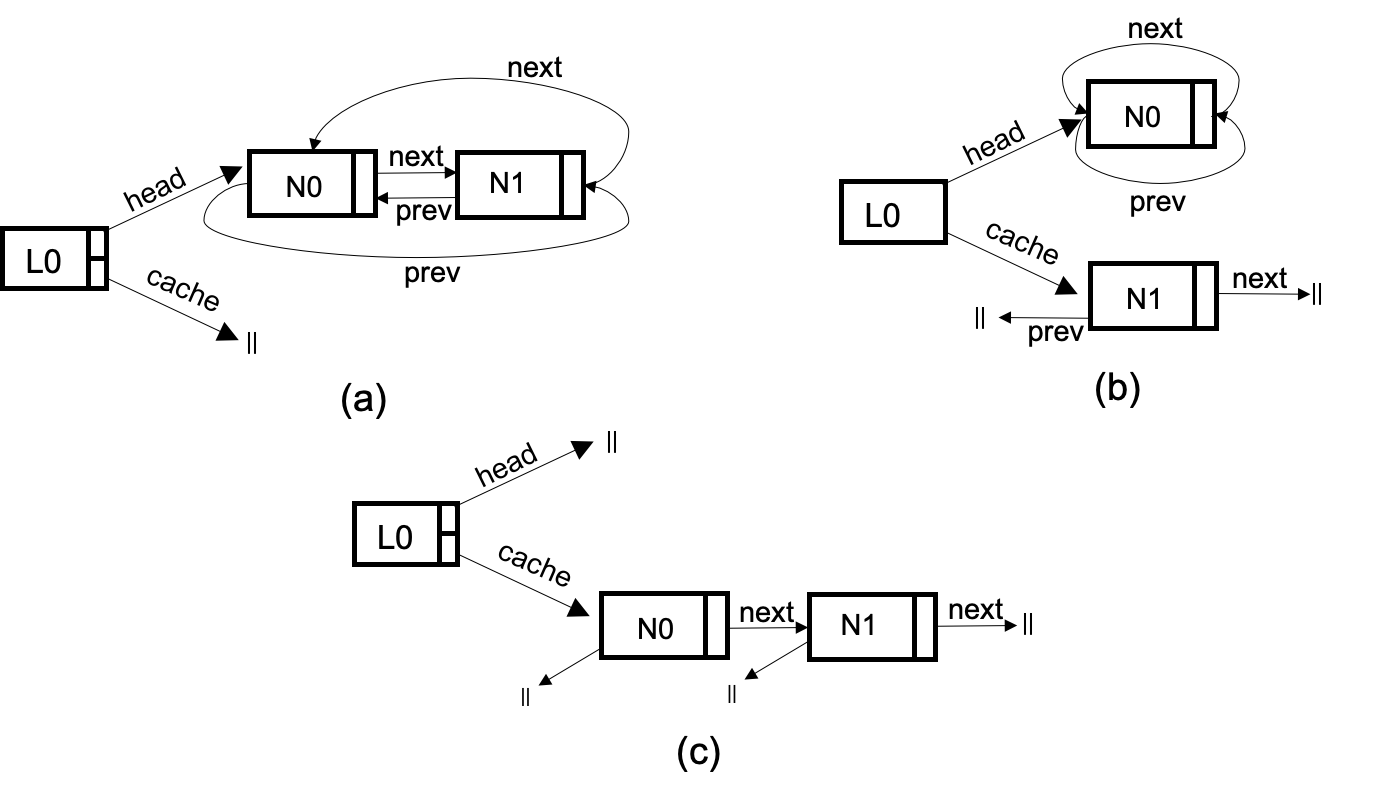
\includegraphics[width=0.85\textwidth]{images/NCL-instances.png}
    \caption{Tres instancias de NodeCachingLinkedList con exactamente dos nodos}
    \label{fig:ncl-instances}
\end{figure}

\begin{figure}[H]
\begin{lstlisting}[keywordstyle=\scriptsize\ttfamily]
max.objects=k
int.range=0:k
strings=str1,str2,str3
omit.fields=NCL.DEFAULT_MAXIMUM_CACHE_SIZE
\end{lstlisting}
\caption{\textsf{BEAPI}'s scope definition for \texttt{NCL} (max. nodes 3)}
\label{fig:NCL-fin-BEAPI}
\end{figure}

En el contexto de la generación exhaustiva acotada, el término \emph{scope} se refiere al límite o alcance que se establece para la generación de estructuras. Es una restricción que define cuántos objetos de un tipo particular pueden aparecer en las estructuras generadas. Esta restricción es esencial para controlar el tamaño y la complejidad del espacio de búsqueda de estructuras durante la generación exhaustiva. Sin un límite en el número de objetos que pueden aparecer en las estructuras generadas, el espacio de búsqueda podría ser infinito o extremadamente grande. Esto hace que la generación sea impracticable en la mayoría de los casos debido al tiempo y los recursos requeridos.  En muchos casos, el conjunto de estructuras relevantes o interesantes es finito y puede definirse mediante un \emph{scope} adecuado. Al generar solo un conjunto finito de estructuras, se pueden abordar de manera exhaustiva todos los casos posibles.

Para limitar el número de estructuras generadas, BEAPI necesita definirlo en un archivo de descripción simple en formato \texttt{java.properties}, en el cual, además, se establecen algunos otros parámetros. En la figura \ref{fig:NCL-fin-BEAPI}, en la línea 1, se puede observar como establecer el \emph{scope} para un caso específico con la sentencia \emph{max.objects}. Este valor (\emph{k}) debe ser un valor entero. Supongamos el caso de la figura \ref{fig:ncl-instances} de instancias de \texttt{NCL}.  El límite $k$ representa el número máximo de objetos que se pueden crear para cada clase (en la Figura \ref{fig:ncl-instances}, el número de nodos en los objetos NCL está acotado por $k=2$). Esto especifica el número máximo de objetos diferentes (alcanzables desde la raíz) permitidos en una estructura. Las secuencias de prueba generadas por \emph{BEAPI} que crean estructuras que exceden este número (para cualquier clase) se descartan y no se siguen extendiendo


Nuestra técnica, basada en generación de test por feedback, necesita, también, un conjunto de valores primitivos especificado por el usuario (enteros, strings, etc) que son utilizados para alimentar a los métodos (que requieran valores primitivos) de la API que se combinan para generar las estructuras del SUT que estamos buscando.
Por ejemplo, en la figura \ref{fig:scope} el método \emph{add(int)}, que agrega un elemento a la lista principal, necesita un entero para el campo \emph{value} de cada nodo. Este valor entero, como es un valor primitivo, se toma de algunos de los valores primitivos que definió el usuario en el archivo de configuración de BEAPI (\ref{fig:NCL-fin-BEAPI}). En la línea 2 y 3 se puede observar que define valores de tipo enteros y valores de tipo string que serán utilizados por los métodos cuando necesiten valores de este tipo. 
\cacho{Explicar sobre objects que son int para nosotros? o esconderlo?}

Cómo último, nuestro archivo de configuración, permite que el usuario especifique que valores desea que no sean tenidos en cuenta a la hora de comparar estructuras. 
Esto toma especial importancia el contexto de estructuras de datos, especialmente en colecciones y contenedores en Java. En estos casos suelen aparecer campos en la clase que representa un contador de modificaciones o cambios realizados en la estructura de datos. Conmútente son llamados \emph{modCount}. Este es un campo que se utiliza para realizar un seguimiento de las modificaciones que se han realizado en la colección desde su creación o desde la última vez que se realizó un seguimiento. El \emph{modCount} es un campo de tipo entero que se incrementa cada vez que se realiza una modificación en la estructura de datos. Las modificaciones pueden incluir inserciones, eliminaciones, actualizaciones u otras operaciones que afecten la colección. El propósito principal de llevar un contador de modificaciones es facilitar la detección de modificaciones concurrentes o cambios inesperados en la colección por parte de múltiples hilos de ejecución. En la línea 4 del archivo de configuración \ref{fig:NCL-fin-BEAPI}, se puede observar como se especifica aquellos campos que deseamos omitir a la hora de tener una representación canónica de la estructura. Canonicalizar un objeto se refiere a la acción de garantizar que un objeto se encuentre en su forma más básica y representativa, lo que facilita las comparaciones y operaciones con otros objetos similares.
Para lograr todo lo explicado en esta sección, nosotros canonizamos los objetos generados por la ejecución de cada secuencia de métodos y analizamos y trabajamos con su representación canónica.
Para finalizar esta sección, se puede observar en la figura \ref{sec:scope} un ejemplo del espacio de búsqueda de una secuencia generada con la combinación del método constructor de la clase más el método \emph{add} de NCL. En esta figura, se especificó un scope de 3. Esto quiere decir que cuando genera alguna estructura con más de 3 nodos como es en el caso de la última secuencia de la figura, esta es descartada por exceder el límite de nodos en la estructura (el nodo ficticio de la estructura se tiene en cuenta en la definición de \emph{scope})
\cacho{Definicion de canonizar y algun ejemplo simple de canonizar?} 

% (Normalmente, las técnicas basada en generación por retroalimentación guardaría los valores primitivos que son devueltos por la ejecución de las pruebas y reutilizaría estos valores en pruebas futuras). También nuestra técnica descartar secuencias de métodos que crean objetos con más de $k$ objetos (de cualquier tipo), para evitar que se construyan objetos más grandes de lo necesario. 






% \cacho{VER BIEN ESTO DE NO EXTENDERSE, porq para crear estrucutras de 3 nodos a veces necesito crear previamente una de 4 nodos}
% Esto asegura que se generen solo \texttt{NCL} con no más de k nodos. Por ejemplo, la figura \ref{fig:scope}, se puede observar que cuando genera una estructura con mas nodos que el especificado en el archivo de configuración, este no sigue extiendo el arbol de búsqueda. En la figura el scope especificado es 3 (vale aclarar, que el nodo ficticio cuanta como nodo de la estructura.)

\begin{figure}[H]
    \centering
    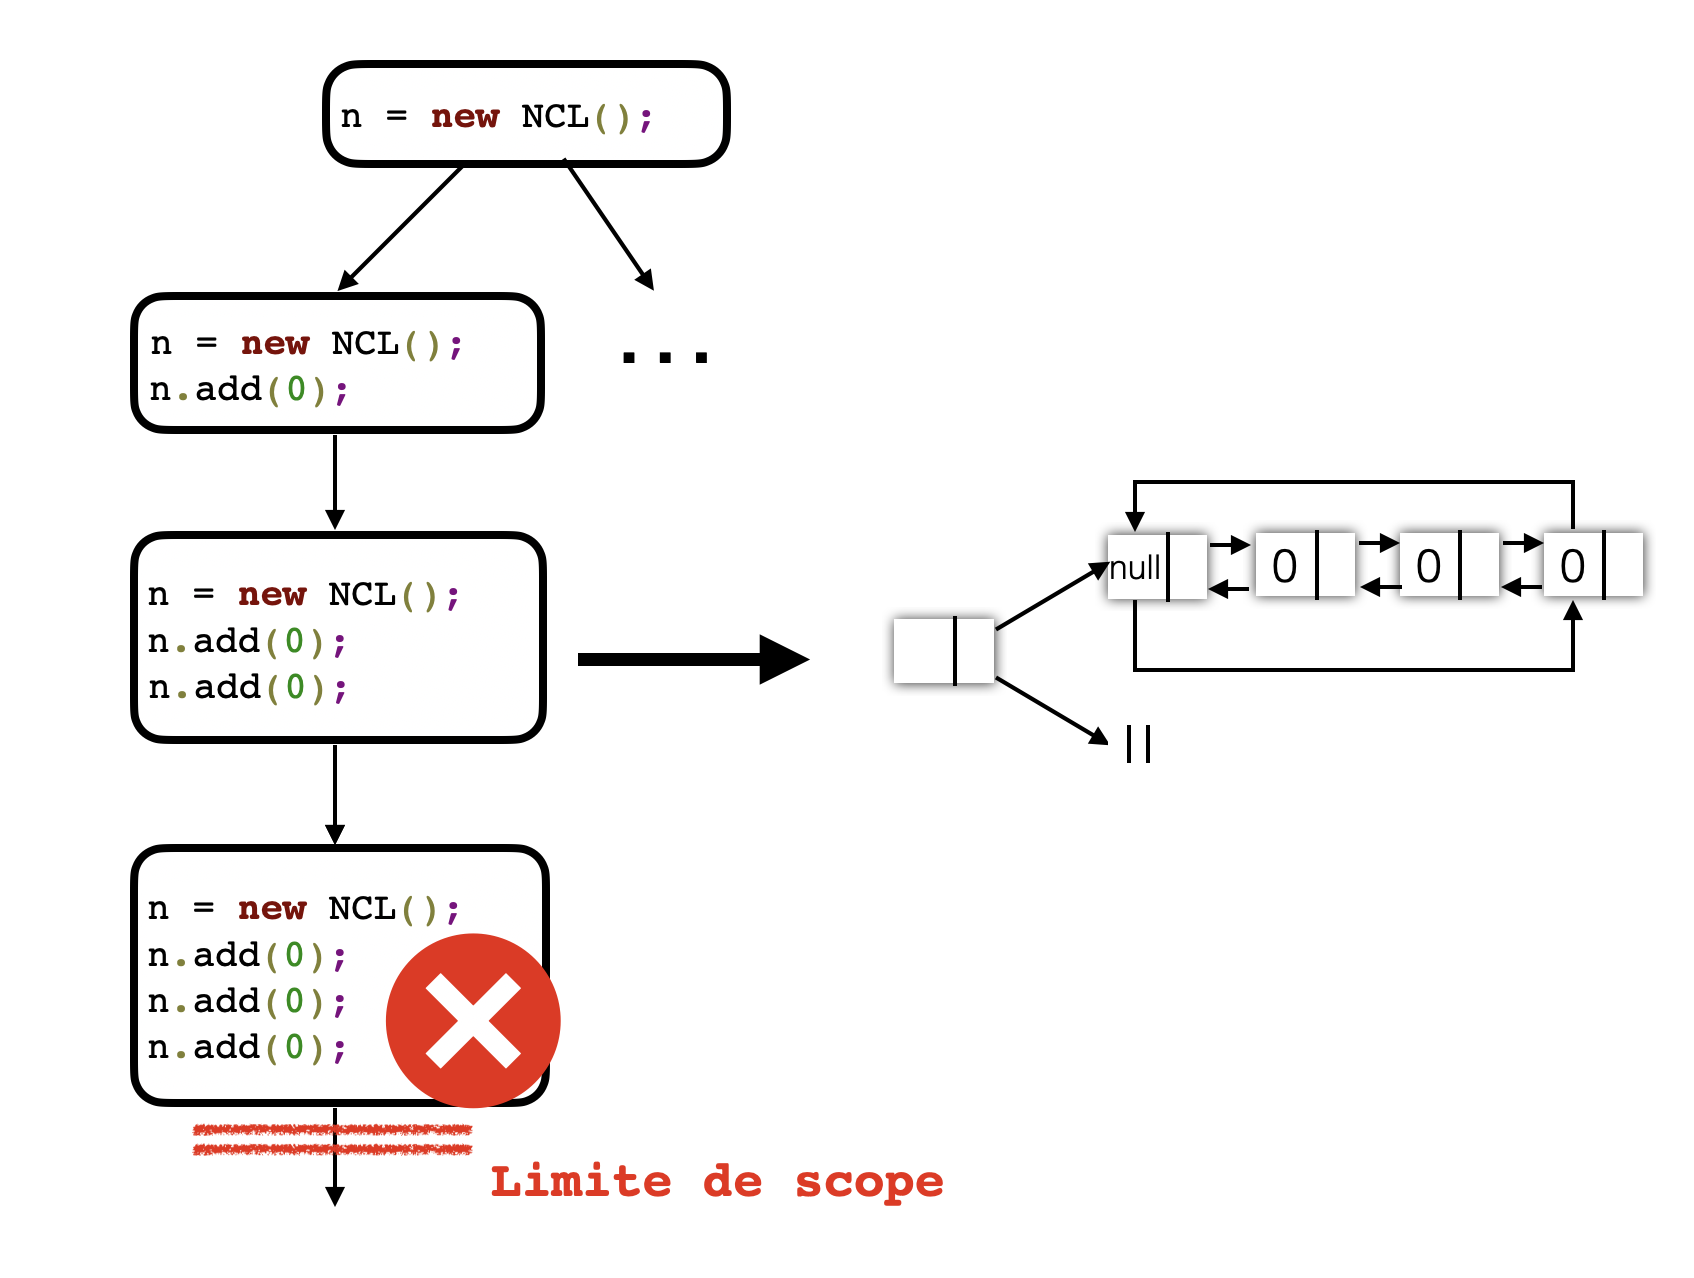
\includegraphics[width=0.85\textwidth]{images/scope.jpg}
    \caption{Representación con scope 3 para NCL}
    \label{fig:scope}
\end{figure}


% Siguiendo el análisis del archivo de configuración de la figura \ref{fig:NCL-fin-BEAPI},
% y el número de valores primitivos disponibles, en nuestro ejemplo de la figura, se especifica enteros del 0 a $k-1$ y cadenas de caracteres: str1, str2, str3. Ademas, se pueden especificar otros valores primitivos como floats, doubles, etc. Esto serán los dominios de datos para los tipos primitivos que necesiten los métodos que serán utilizados. Podemos indicarle a \emph{BEAPI} que ignore algunos campos en el proceso de canonización de objetos, que se lleva a cabo en la ejecución de las secuencias de métodos de la API. Esto permite al usuario controlar qué partes de la estructura del objeto son relevantes para la coincidencia de estados (ver más adelante en la sección \ref{sec:stateMatching}). Por ejemplo,  la línea 4 haría que \emph{BEAPI} omita el tamaño máximo predeterminado de la caché en la coincidencia de estados, que en la API de \emph{NCL} es una constante inicializada en 20 en el constructor de la clase. Es importante que aqui se omitan campos que puede afectar la coincidencia de estados, como el caso del campo \emph{modCount}. Esta variable se utiliza a menudo en estructuras de datos para realizar un seguimiento de las modificaciones o cambios realizados en los datos almacenados, pero claramente no afecta la estructura generada. 
% La configuración mostrada en la Figura~\ref{fig:NCL-fin-BEAPI} es suficiente para que \emph{BEAPI} genere NCL con un máximo de 3 nodos, que contienen enteros del 0 al 2 como valores. 


\section{State Matching}
\label{sec:stateMatching}

En la generación de objetos con \textsf{BEAPI}, a menudo muchas secuencias de prueba producen la misma estructura. Por ejemplo, en la figura \ref{fig:stateMatching}, insertar un elemento en una lista y luego eliminarlo . \textsf{BEAPI} asume que las ejecuciones de métodos son deterministas, es decir, cualquier ejecución de una rutina con las mismas entradas produce los mismos resultados. Observamos que para cada estructura distinta $s$, solo necesitamos guardar la primera secuencia de prueba que genera $s$ (y la estructura en sí). Todas las secuencias de prueba generadas posteriormente que también crean $s$ pueden ser descartadas. Si almacenamos muchas secuencias de prueba para la misma estructura, todas estas secuencias tendrían que ser extendidas con nuevas rutinas en iteraciones posteriores de \textsf{BEAPI}, lo que resultaría en extensiones innecesarias. Por lo tanto, implementamos la coincidencia de estados en \textsf{BEAPI} de la siguiente manera.

\begin{figure}[H]
    \centering
    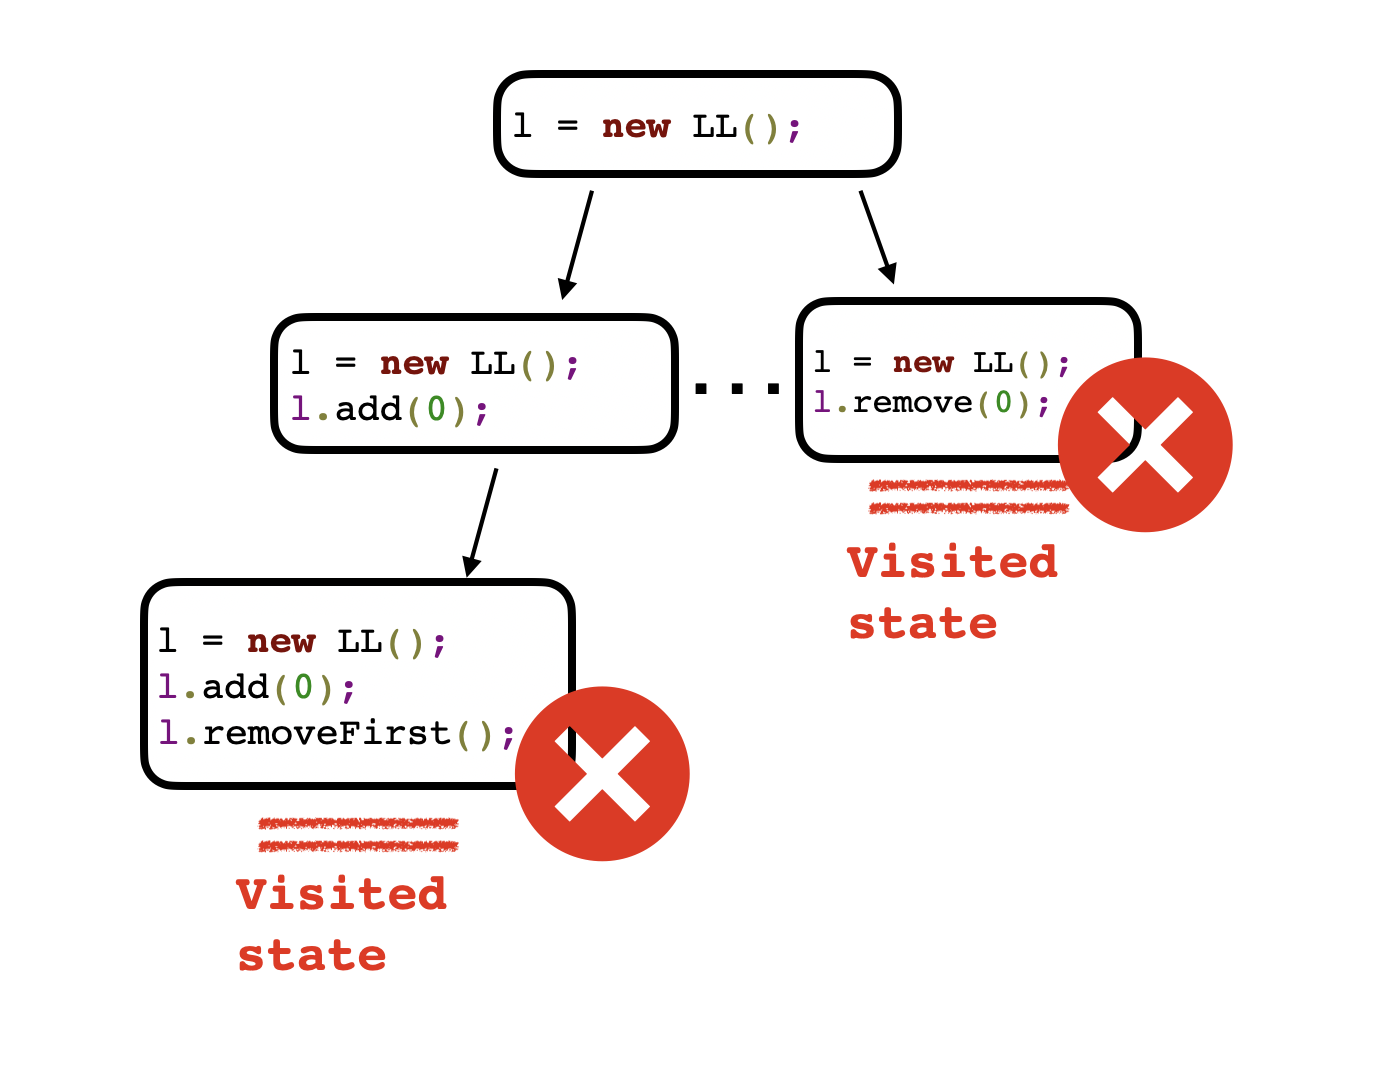
\includegraphics[width=0.85\textwidth]{images/stateMatching.jpg}
    \caption{Representación con scope 3 para NCL}
    \label{fig:stateMatching}
\end{figure}

Almacenamos todas las estructuras producidas hasta ahora por \textsf{BEAPI} en una forma canónica (ver más abajo). Después de ejecutar la última rutina \texttt{r(p$_1$, ..., p$_k$)} de una nueva secuencia de prueba generada \texttt{T}, comprobamos si alguno de los parámetros de \texttt{r} tiene una estructura no vista antes (no almacenada). Si \texttt{T} no crea ninguna estructura nueva, se descarta. De lo contrario, \texttt{T} y las nuevas estructuras que genera son almacenadas por \textsf{BEAPI}.

Representamos las estructuras asignadas en el heap como grafos etiquetados. Después de la ejecución de un método, un parámetro $p$ (de tipo no primitivo) contiene una referencia al objeto raíz $r$ de un \emph{heap} con raíz (es decir, $p=r$), definido a continuación.

\begin{definition}
Sea $O$ un conjunto de objetos y $P$ un conjunto de valores primitivos (incluido $null$). Sea $F$ el conjunto de campos de todos los objetos en $O$.
\begin{itemize}
\item Un \emph{heap} es un grafo etiquetado $H = \langle O, E\rangle$ con $E = {(o, f, v) | o \in O, f \in F, v \in O \cup P}$.
\item Un \emph{heap con raíz} es un par $RH = \langle r, H \rangle$ donde $r \in O$, $H = \langle O, E\rangle$ es un heap, y para cada $v' \in O \cup P$, $v'$ es alcanzable desde $r$ a través de campos en $F$.
\end{itemize}
\end{definition}

El caso especial $p = null$ se puede representar con un \emph{heap} con raíz que tiene un nodo ficticio y un campo ficticio que apunta a null. En lenguajes como Java, cada objeto se identifica por la dirección de memoria donde se encuentra. Cambiar las direcciones de memoria donde se asignan los objetos no tiene efecto desde el punto de vista del programa, ya que el programador no tiene control sobre la representación de bajo nivel de la memoria (a diferencia de otros lenguajes como C). Los \emph{heaps} obtenidos mediante permutaciones de las direcciones de memoria de sus objetos componentes se llaman \emph{heaps isomorfos}. Evitamos la generación de \emph{heaps isomorfos} empleando una representación canónica para los heaps \cite{Iosif02,Boyapati02}. Los heaps con raíz se pueden canonizar eficientemente mediante un enfoque llamado \emph{linearización} \cite{Iosif02,Xie04}, que transforma un heap con raíz en una secuencia única de valores.

\bigbreak

\begin{figure}[!th]
\begin{lstlisting}
int[] linearizar(O raiz, Heap<O, E> heap, int alcance, Regex omitirCampos) {
    Map ids = new Map(); // mapea nodos a sus identificadores unicos
    return lin(raiz, heap, alcance, ids, omitirCampos);
}
int[] lin(O raiz, Heap<O, E> heap, int alcance, Map ids, Regex omitirCampos) {
    if (ids.containsKey(raiz))
        return secuenciaUnica(ids.get(raiz));
    if (ids.size() == alcance)
        throw new ExcepcionAlcanceSuperado();
    int id = ids.size() + 1;
    ids.put(raiz, id);
    int[] seq = secuenciaUnica(id);
    Edge[] campos =
    ordenarPorCampo({ <raiz, f, o> en E }, omitirCampos);
    foreach (<raiz, f, o> en campos) {
        if (esPrimitivo(o))
            seq.add(representacionUnica(o));
        else
            seq.append(lin(o, heap, alcance, ids, omitirCampos));
    }
    return seq;
}
\end{lstlisting}
\caption{Algoritmo de linearización}
\label{alg:linearization}
\end{figure}


% java.util.LinkedList.MAX_ARRAY_SIZE&java.util.LinkedList:0&2147483639
% java.util.LinkedList.first&java.util.LinkedList:0&java.util.LinkedList$Node:0
% java.util.LinkedList.last&java.util.LinkedList:0&java.util.LinkedList$Node:1
% java.util.LinkedList.modCount&java.util.LinkedList:0&2
% java.util.LinkedList.serialVersionUID&java.util.LinkedList:0&876323262645176354
% java.util.LinkedList.size&java.util.LinkedList:0&2
% traversal.DummyHeapRoot.theroot&traversal.DummyHeapRoot:0&java.util.LinkedList:0



El algoritmo mostrado en la Figura~\ref{alg:linearization} es una versión personalizada para \textsf{BEAPI} del algoritmo de linearización presentado en \cite{Xie04}. Esta versión ha sido modificada para informar cuando los objetos exceden los alcances y para permitir la omisión de campos de objeto.

El algoritmo \texttt{linearize} invoca a la función \texttt{lin} y realiza un recorrido en profundidad del heap comenzando desde la raíz (línea 3). Durante este recorrido, se asignan identificadores diferentes a cada objeto visitado. Cuando se visita un objeto por primera vez, se le asigna un nuevo identificador único (líneas 10-11) y se crea una secuencia de un solo elemento llamada \texttt{seq}, que contiene el identificador de objeto y representa el objeto (línea 12). El mapa \texttt{ids} se utiliza para almacenar el mapeo entre los objetos y los identificadores de objeto únicos.

A continuación, se recorren los campos del objeto en un orden predefinido (por ejemplo, por nombre) y se construye la linearización de cada valor de campo, que se agrega a la secuencia \texttt{seq} (líneas 13-19). Si un campo almacena un valor primitivo (línea 15), se agrega una secuencia de un solo elemento que representa ese valor a \texttt{seq} (línea 16). Si el campo hace referencia a otro objeto, se realiza una llamada recursiva a la función \texttt{lin} para transformarlo en una secuencia, que luego se agrega a \texttt{seq} (línea 18).

Al final del ciclo, la secuencia \texttt{seq} contiene la representación canónica de todo el heap que comienza en la raíz, y se devuelve por la función \texttt{lin} (línea 20). Sin embargo, si se encuentra un objeto que ya ha sido visitado en llamadas recursivas anteriores, es decir, que ya tiene un identificador asignado en \texttt{ids}, el algoritmo devuelve una secuencia de un solo elemento que contiene el identificador único del objeto (líneas 6-7).

Si hay más de \texttt{scope} objetos alcanzables desde la raiz del \emph{heap}, lo cual significa que se ha superado el límite establecido en los alcances, el algoritmo \texttt{linearize} devuelve una excepción para informar esta situación (líneas 9-10). Además, el parámetro \texttt{linearize} también acepta una expresión regular llamada \texttt{omitFields}, que se utiliza para coincidir con los nombres de los campos que deben ser omitidos durante la canonización del \emph{heap}.

Para omitir dichos campos, se implementa la función \texttt{sortByField} (línea 13) de manera que no se devuelven las aristas correspondientes a los campos cuyos nombres coinciden con \texttt{omitFields}. Es importante destacar que este comportamiento es específico de nuestro enfoque, ya que la excepción será utilizada por \textsf{BEAPI} para descartar secuencias de prueba que generen objetos que excedan los alcances permitidos.

Cabe destacar que la linearización proporciona una forma eficiente de comparar objetos: dos objetos se consideran iguales si y solo si las secuencias correspondientes generadas por la función \texttt{linearize} son iguales.


\section{Uso de Builders en BEAPI}
\label{sec:builders}
En esta sección, introducimos una optimización que hemos desarrollado y que es una parte importante de esta tesis. Explicaremos una de las formas en las que utilizamos una técnica llamada \emph{identificación de métodos builders} en una API. Estos métodos builders nos permiten generar una gran diversidad de objetos (pudiendo generar de manera exhaustiva, es decir, generando todos los objetos posibles hasta un alcance dado).

Dado que la cantidad de combinaciones factibles de métodos crece de manera exponencial con el número de métodos, es crucial reducir la cantidad de métodos que \textsf{BEAPI} utiliza para producir secuencias de prueba. Para abordar este problema, utilizamos un enfoque de identificación automática de métodos builders que se describe en el capítulo siguiente (Capítulo \ref{cap:builders}). Este enfoque nos ayuda a encontrar un subconjunto de métodos de la API que son suficientes para generar conjuntos de estructuras acotadas y exhaustivas. En el contexto de \textsf{BEAPI}, utilizamos un algoritmo de búsqueda de tipo Greedy para identificar este subconjunto de builders.

En esta sección, presentamos un enfoque más simple basado en el algoritmo de optimización Hill Climbing (HC) que logra un mejor rendimiento. Aunque HC puede ser menos preciso, ya que puede incluir algunos métodos que no son necesarios para producir un conjunto acotado y exhaustivo de estructuras, en nuestros experimentos, HC funcionó muy bien y calculó consistentemente conjuntos mínimos de builders (verificamos que coincidieran con los builders identificados manualmente en cada estudio de caso). Nuestro objetivo aquí es evaluar el impacto de utilizar builders para la generación exhaustiva acotada (BEG) a partir de una API.

Para la identificación de métodos builders, utilizamos una función de evaluación que emplea un generador exhaustivo para crear objetos de la API (ver sección \ref{sec:fitness}). El algoritmo Hill Climbing realiza múltiples invocaciones a este generador exhaustivo durante la identificación de los builders.

La idea clave que hace posible la identificación eficiente de builders es que a menudo los builders identificados para un alcance relativamente pequeño son los mismos que se necesitan para crear estructuras de cualquier tamaño. En otras palabras, una vez que el alcance es lo suficientemente grande para computar los builders, aumentar aún más el alcance no modificará el conjunto de builders. Este resultado se asemeja a la hipótesis del alcance pequeño para la detección de errores \cite{Andoni02} (y a la técnica de "transcoping" \cite{Rosner13}). En todos nuestros casos de estudio, un alcance de 5 fue suficiente para calcular los builders (verificamos manualmente la corrección de los builders en todos los casos). Después de identificar eficientemente los builders con un alcance pequeño, podemos ejecutar \textsf{BEAPI} utilizando los builders identificados y un alcance mayor. Esto nos permite generar objetos más grandes y utilizarlos para probar el SUT.

En la mayoría de nuestros casos de estudio, los builders consisten en un constructor y un solo método para agregar elementos a la estructura. Sin embargo, nuestro enfoque automatizado de identificación de builders mostró que, en el caso de los árboles Rojo-Negro, también se requería un método de eliminación (para alcances mayores que 3). Esto se debe a que existen árboles con una configuración específica de equilibrio (coloreando los nodos en rojo y negro) que no se pueden construir solo agregando elementos al árbol. En contraste, los árboles AVL, que también son estructuras balanceadas, no requieren el método de eliminación como parte de su builder; solo el constructor de la clase y una rutina de adición son suficientes. Esto demuestra que la identificación de builders no es trivial de realizar manualmente.

Para obtener más información sobre esta sección, invitamos al lector a leer el siguiente capítulo donde se explica en detalle el desarrollo de esta técnica (Capítulo \ref{cap:builders}).

\section{Algoritmo de BEAPI}
\label{sec:beapiTechnique}

A continuación se muestra un pseudocódigo de \emph{BEAPI} en la Figura \ref{alg:beapi}. \emph{BEAPI} toma como entradas una lista de métodos de una API,  \texttt{methods}. Estos metodos pueden ser la API completa o un subconjuntos de metodos de la misma. En nuestro caso, como hemos aplicado anteriormente, vamos a utilizar los métodos \emph{builders} previamente identificados. Ademas, el algoritmo toma el alcance (scope) de objetos para la generación, \texttt{scope}; una lista para crear valores de cada tipo primitivo proporcionado en la descripción del alcance, \texttt{primitives} (creados automáticamente a partir de las opciones de configuración como \texttt{int.range}, \texttt{string}, etc., ver Figura~\ref{fig:NCL-fin-BEAPI}); y una expresión regular que coincide con los campos que se deben omitir en la canonización de las estructuras, \texttt{omitFields}. Notar que se pueden pasar métodos de más de una clase en \texttt{methods} si se desean generar objetos para varias clases en la misma ejecución de \textsf{BEAPI}, por ejemplo, cuando los métodos de una clase toman objetos de otra clase como parámetros. La estructura de datos de tipo Map, \texttt{currSeqs} de \emph{BEAPI}  almacena, para cada tipo, la lista de secuencias de test que se sabe que generan estructuras del tipo correspondiente. El \cacho{check}\texttt{currSeqs} se inicia con todas las secuencias de tipos primitivos en \texttt{primitives} (líneas 3-4). En cada iteración del bucle principal (líneas 6-39), \textsf{BEAPI}  crea nuevas secuencias para cada método disponible \texttt{m} (línea 9), explorando exhaustivamente todas las posibilidades para crear secuencias de prueba utilizando \texttt{m} e inputs generados en iteraciones anteriores y almacenados en \texttt{currSeqs} (líneas 10-35). Las secuencias de prueba recién creadas que generan nuevas estructuras en la iteración actual se guardan en el mapa \texttt{newSeqs} (inicializado vacío en la línea 7). Se puede observar que todas las secuencias generadas se agregan a \texttt{currSeqs} al final de la iteración principal (línea 40). Si no se producen nuevas estructuras en la iteración actual (\texttt{newStrs} es falso en la línea 36), el bucle principal del algoritmo de  \textsf{BEAPI}  termina su ejecución y se devuelve la lista de todas las secuencias en \texttt{currSeqs} (línea 40).


\begin{figure}[t!]

\begin{lstlisting}[language=Java]
public BEAPI(List methods, int scope, Map<Type, List<Seq>> primitives, 
Regex omitFields) {
    Map<Type, List<Seq>> currSeqs = new Map();
    currSeqs.addAll({ T->L | T->L in primitives });
    Set canonicalStrs = new Set();
    for (int it=0; true; it++) {
      Map<Type, List<Seq>> newSeqs = new Map();
      boolean newStrs = false;
      for (m(T1,...,Tn):Tr: methods) {
        Map<Type, List<Seq>> seqsT1 = currSeqs.getSequencesForType(T1);
        ...
        Map<Type, List<Seq>> seqsTn = currSeqs.getSequencesForType(Tn);
        for ((s1,...,sn): seqsT1 x ... x seqsTn) {
          Seq newSeq = createNewSeq(s1,...,sn,m);
          o1,...,on,or,failure,exception = execute(newSeq);
          if (failure) 
            throw new ExecutionFailedException(newSeq);
          if (exception) 
            continue;
          c1,...,cn,cr,outOfScope = makeCanonical(o1,...,on,scope,omitFields);
          if (outOfScope) 
            continue;
          if (isReferenceType(T1) and !canonicalStrs.contains(c1)) {
                canonicalStrs.add(c1);
                newSeqs.addSeqForType(T1, newSeq);
                newStrs = true;
          }
          ...
          if (isReferenceType(Tr) and !canonicalStrs.contains(cr)) {
                canonicalStrs.add(cr);
                newSeqs.addSeqForType(Tr, newSeq);
                newStrs = true;
          }
        }
      }
      if (!newStrs) 
        break;
      currSeqs.addAll(newSeqs);
    }
    return currSeqs.getAllSeqsAsList();
}
\end{lstlisting}
\caption{\textsf{BEAPI} algorithm}
\label{alg:beapi}
\end{figure}

A continuación, comentaré los detalles del bucle for en las líneas 9-35. En primer lugar, se obtienen todas las secuencias que se pueden utilizar para construir entradas para \texttt{m} en \texttt{seqsT$_1$}, ..., \texttt{seqsT$_n$}. \textsf{BEAPI} explora cada tupla \texttt{(s$_1$}, ..., \texttt{s$_n$)} de entradas factibles para \texttt{m}. A continuación, se ejecuta \texttt{createNewSeq} (línea 14), que construye una nueva secuencia de prueba \texttt{newSeq} realizando la composición secuencial de las secuencias de prueba \texttt{s$_1$}, ..., \texttt{s$_n$} y la rutina \texttt{m}, y reemplazando los parámetros formales de \texttt{m} por las variables que crean los objetos requeridos en \texttt{s$_1$}, ..., \texttt{s$_n$}. Luego, se ejecuta \texttt{newSeq} (línea 15) y como resultado podemos tener que, produzca un fallo (\texttt{failure} se establece en verdadero), genera una excepción que representa un uso no válido de la API (\texttt{exception} se establece en verdadero) o su ejecución tiene éxito y crea nuevos objetos \texttt{o$_1$,$\ldots$,o$_n$}. En caso de fallo, se lanza una excepción y \texttt{newSeq} se presenta al usuario como evidencia del fallo (línea 17). Si se lanza un tipo diferente de excepción, \textsf{BEAPI} asume que corresponde a un mal uso de la API (ver más abajo), descarta la secuencia de prueba (línea 19) y continúa con la siguiente secuencia candidata. De lo contrario, la ejecución de \texttt{newSeq} genera nuevos objetos \texttt{o$_1$,$\ldots$,o$_n$} (o valores de tipos primitivos) que se canonizan mediante \texttt{makeCanonical} (línea 20) --ejecutando \texttt{linearize} de la Figura~\ref{alg:linearization} en cada estructura. Si alguna de las estructuras producidas por \texttt{newSeq} excede el scope, \texttt{makeCanonical} establece \texttt{outOfScope} en verdadero, \textsf{BEAPI} descarta \texttt{newSeq} y continúa con la siguiente (línea 22).
Esto garantiza que \textsf{BEAPI} nunca crea objetos más grandes que lo permitidio por el alcance.
Si ninguna de las situaciones anteriores ocurre, quiere decir que ha pasado todos los chequeos la secuencia corriente y, \texttt{makeCanonical} devuelve versiones canónicas de \texttt{o$_1$,$\ldots$,o$_n$} en las variables \texttt{c$_1$,$\ldots$,c$_n$}, respectivamente. A continuación, \textsf{BEAPI} realiza una coincidencia de estado comprobando que la estructura canónica \texttt{c$_1$} sea de tipo de referencia y que no haya sido creada por ninguna secuencia de prueba anterior (línea 23). Observa que \texttt{canonicalStrs} almacena todas las estructuras ya visitadas. Si \texttt{c$_1$} es una nueva estructura, se agrega a \texttt{canonicalStrs} (línea 24) y se agrega la secuencia que crea \texttt{c$_1$}, \texttt{newSeq}, al conjunto de secuencias de prueba que producen estructuras de tipo \texttt{T$_1$} (\texttt{newSeqs} en la línea 27). Además, se establece \texttt{newStrs} en verdadero para indicar que al menos se ha creado un nuevo objeto en la iteración actual (línea 26). Este proceso se repite para los objetos canónicos \texttt{c$_2$,$\ldots$,c$_n$,c$_r$} (líneas 29-32).
\cacho{Un for aqui}

\textsf{BEAPI} distingue los fallos del mal uso de la API en función del tipo de excepción (similarmente a las técnicas anteriores de generación de pruebas basadas en API \cite{Pacheco07}). Por ejemplo,\\
\texttt{IllegalArgumentException} y \texttt{IllegalStateException} corresponden a usos incorrectos de la API, y el resto de las excepciones se consideran fallos de manera predeterminada. La implementación de \textsf{BEAPI} permite al usuario seleccionar las excepciones que corresponden a fallos y aquellas que no, configurando los parámetros correspondientes. Como se mencionó en la Sección~\ref{sec:motivating-example}, \textsf{BEAPI} asume que los métodos de la API lanzan excepciones cuando no se pueden ejecutar con entradas inválidas. Sostenemos que esta es una práctica común, llamada programación defensiva \cite{Liskov00}, que todos los programadores deberían seguir, ya que resulta en un código más robusto y mejora las pruebas de software en general \cite{Ammann16} (además de ayudar a las herramientas de generación de pruebas automatizadas). También argumentamos en la Sección~\ref{sec:motivating-example} que el esfuerzo de especificación requerido para la programación defensiva es mucho menor que escribir \texttt{repOK}s precisos (y eficientes) para BEG, y esto era cierto después de inspeccionar manualmente el código fuente de nuestros casos de estudio. Por otro lado, ten en cuenta que \textsf{BEAPI} puede utilizar especificaciones formales para revelar errores en la API, por ejemplo, ejecutando \texttt{repOK} y comprobando que devuelve verdadero en cada objeto generado del tipo correspondiente (como en Randoop \cite{Pacheco07}). Sin embargo, las especificaciones utilizadas para encontrar errores no necesitan ser muy precisas (por ejemplo, el \texttt{repOK} subespecificado de \texttt{NCL} de la Sección~\ref{sec:motivating-example} es válido para encontrar errores), ni estar escritas de una manera particular (como lo requiere \textsf{Korat}). \textsf{BEAPI} también puede utilizar otros tipos de especificaciones más débiles y más simples de escribir para revelar errores, como violaciones de contratos específicos del lenguaje (por ejemplo, \texttt{equals} es una relación de equivalencia en Java), propiedades metamórficas \cite{Chen19}, afirmaciones proporcionadas por el usuario (\texttt{assert}), etc.

Otra ventaja de \textsf{BEAPI} es que, para cada objeto generado, proporciona una secuencia de prueba que se puede ejecutar para crear el objeto. Esto contrasta con los enfoques basados en especificaciones (que generan un conjunto de objetos a partir de \texttt{repOK}). Encontrar una secuencia de invocaciones a métodos de la API que creen una estructura específica es un problema difícil en sí mismo, que puede ser bastante costoso computacionalmente \cite{Braione17} o requerir un esfuerzo significativo para realizarlo manualmente. Por lo tanto, a menudo los objetos generados por enfoques basados en especificaciones están "incrustados" cuando se utilizan para probar un SUT (por ejemplo, mediante el uso de reflexión en Java), lo que hace que las pruebas sean muy difíciles de entender y mantener, ya que dependen de los detalles de implementación de bajo nivel de las estructuras \cite{Braione17}.






%!TEX root = main.tex
\chapter[Evaluaci\'on]{Evaluaci\'on}
\label{cap:experimental}



En los capítulos \ref{cap:builders} y \ref{cap:beapi} presentamos varios enfoques para mejorar la generación exhaustiva acotada:

\begin{itemize}
\item Identificación de métodos generadores para construir todos los objetos disponibles hasta una cota en una API. En este sentido, presentamos los siguientes algoritmos para encontrar estos métodos:
\begin{itemize}
\item Algoritmo Genético.
\item Algoritmo Perezoso.
\item Algoritmo basado en clases de equivalencia.
\end{itemize}
\item Generación exhaustiva acotada a partir de métodos de la API.
\end{itemize}

En este capítulo, realizamos una evaluación experimental de estas técnicas con el objetivo de analizar la eficiencia y efectividad de las suites producidas en comparación con la generación exhaustiva acotada. En otras palabras, las siguientes preguntas de investigación guían esta experimentación:

\cacho{TODO: pensar mejor las RQ}
\begin{itemize}
\item \emph{RQ1}: ¿Qué tan eficientes son los algoritmos (Algoritmo Genético, \emph{Hill Climbing}, Clases de Equivalencia) para identificar conjuntos de métodos suficientes? 
\item \emph{RQ2}: ¿Qué tan efectivos son los algoritmos presentados para identificar conjuntos de métodos generadores de objectos suficientes de cada API?
¿Cuánto tiempo computacional requiere cada enfoque?
\item \emph{RQ3}: ¿Cuál es el impacto de utilizar métodos Builders identificados en comparación con el uso de todos los métodos de la API en el contexto de verificación de software?
\item \emph{RQ4}: ¿Puede realizarse eficientemente la generación exhaustiva utilizando métodos de la API (BEAPI)?
\item\emph{RQ4}: ¿Cuál es el impacto de las optimizaciones propuestas en el rendimiento de BEG a partir de la API?
\item\emph{RQ6}: ¿Puede BEAPI ayudar a encontrar discrepancias entre las especificaciones repOK y la capacidad de generación de objetos de la API?
\item\emph{RQ7}: ¿Qué tan efectivas son las suites de prueba reducidas en comparación con la generación exhaustiva acotada?
\end{itemize}

% \section{Algoritmos de Identificacion de metodos builders}


\section{Evaluación Experimental en identificación de métodos builders}
\label{sec:buildersExp}
En esta sección, evaluamos experimentalmente nuestros enfoques presentados en el capítulo \ref{cap:builders}. Describiremos como es la eficiencia y efectividad de cada algoritmo con las funciones de valoración presentada en la sección \ref{sec:fitness}. Además, mostraremos el uso de estos métodos identificados por nuestras técnicas durante el uso de una herramienta de verificación de software.

La evaluación se basa en un conjunto de implementaciones de estructuras de datos que se utilizan como referencia, incluyendo: \verb"NCL" de Apache Collections \cite{apache}; \verb"BinaryTree", \verb"BinomialHeap", \verb"FibonacciHeap" tomados de \cite{Visser:2006}; \verb"UnionFind", una implementación de conjuntos disjuntos tomada de JGrapht \cite{jgrapht}. También evaluamos nuestra técnica en componentes de proyectos de software reales, como \verb"Lits" de la implementación de Sat4j \cite{sat4j}, tomada de \cite{Loncaric:2018}, que consiste en un almacén de variables que controla cuándo se realizó la última suposición sobre el valor de una variable y si hay oyentes observando el estado de esa variable; \verb"Scheduler", una implementación de un planificador de procesos tomada de \cite{sir}; y estructuras de datos conocidas del paquete \verb"java.util" \footnote{https://docs.oracle.com/javase/8/docs/api/java/util/package-summary.html} como: \verb"TreeMap", \verb"TreeSet", \verb"HashMap", \verb"HashSet" y \verb"LinkedList". 

Para corroborar nuestros resultados, necesitamos conocer cuáles son los métodos builders mínimos y suficiente de cada caso de estudio. Para esto hemos creado un \emph{ground Truth} manualmente. Fue necesario inspeccionar cada caso de manera manual. Esto llevo un largo trabajo para estudiar los casos de estudio más complejo. El \emph{ground truth} de nuestros casos de estudios se pueden observar en la tabla \ref{tab:groundTruth}. Esta incluye el número de rutinas en la API completa (\#API), y el conjunto de los \emph{builders} identificados manualmente (algunos métodos pueden intercambiarse en diferentes ejecuciones, por ejemplo, \texttt{addFirst} y \texttt{addLast} en NCL)
    
Todos los experimentos se ejecutaron en máquinas Intel Core i7-6700 de 3.4 GHz con 8GB de RAM, utilizando GNU/Linux como sistema operativo. 

\begin{table}[t!]
\centering
{\scriptsize
\begin{tabular}{l l}
\hline
&Métodos generadores de objectos  \\
\hline
\multirow{2}{*}{\textbf{NCL}} 
 & NCLinkedList(int)  \\
 & addFirst(Object)    \\
 {\scriptsize \#API: 34} & removeFirst()  \\
\hline

\multirow{2}{*}{\textbf{UFind}} 
 & UnionFind()  \\
 & addElement(int)   \\
 {\scriptsize \#API: 9} & union(int,int)   \\
\hline

\multirow{2}{*}{\textbf{FHeap}} 
 & FibonacciHeap()  \\
 & insert(int)  \\
 {\scriptsize \#API: 7} & removeMin()  \\
\hline
\multirow{1}{*}{\textbf{BTree}} 
 & BinTree()  \\
 {\scriptsize \#API: 7} & add(int) \\
\hline

\multirow{1}{*}{\textbf{BHeap}} 
 & BinomialHeap()  \\
 {\scriptsize \#API: 10} & insert(int) \\
 & decreaseKeyValue(int,int)   \\
\hline

\multirow{5}{*}{\textbf{Lits}} 
 & Lits() \\
 & getFromPool(int) \\
 & satisfies(int)  \\
 & forgets(int) \\
 {\scriptsize \#API: 26} & setLevel(int,int)  \\
 & setReason(int)\\
\hline

\multirow{3}{*}{\textbf{Sched.}} 
 & Schedule() \\
 & addProcess(int) \\
{\scriptsize \#API: 10} & blockProcess() \\
%  & quantumExpire() & \\
%   & finishProcess() & \\

\hline

\multirow{1}{*}{\textbf{LinkedList}} 
 & LinkedList() \\
 {\scriptsize \#API: 67} & addFirst(Object)  \\
 \hline

\multirow{2}{*}{\textbf{TreeMap}} 
 & TreeMap() \\
 & put(Object,Object) \\
{\scriptsize \#API: 61} & remove(Object) \\
\hline

\multirow{2}{*}{\textbf{TreeSet}} 
 & TreeSet() \\
 & add(Object) \\
{\scriptsize \#API: 34} & remove(Object) (int) \\
\hline

\multirow{1}{*}{\textbf{HashSet}} 
 & HashSet(int,float) \\
 {\scriptsize \#API: 31} & add(Object) \\
\hline

\multirow{1}{*}{\textbf{HashMap}} 
 & HashMap(int,float)  \\
{\scriptsize \#API: 45} & put(Object,Object)  \\
\hline

\end{tabular}%
}
\caption{Ground truth de métodos generadores por clase y la cantidad de métodos en la API de cada clase.}
\label{tab:groundTruth}
\end{table}


\subsection{Parámetros y Evaluación}
Como se discutió en el capítulo \ref{cap:beapi}, es necesario configurar ciertos parámetros para el funcionamiento de nuestros algoritmos y funciones de valoración. Los parámetros más importantes que afectan la eficiencia y efectividad de nuestro algoritmo genético son la tasa de mutación y de cruce, el tamaño de la población y el número de torneos en la selección. 

Para nuestra función objetivo donde medimos cobertura a partir de test suites generadas por Randoop \ref{sec:fitnessRandoop}, es importante conocer el tiempo disponible para generar objetos. Además, Randoop  necesita de una semilla. Esta semilla en Randoop se utiliza para controlar la generación de pruebas aleatorias y permite reproducir los mismos resultados en ejecuciones posteriores si utilizas la misma semilla. Esto puede ser útil para la reproducibilidad y comparación de resultados en el contexto de pruebas de software. Los resultados de Randoop, siempre tiene una aleatoriedad que, entre otras cosas, depende de esta semilla. En nuestros experimentos, cada vez que ejecutamos nuestra técnica, elegimos aleatoriamente una semilla para poder ver como se comporta. 
En cuanto a la función de valoración que se utiliza un generador exhaustivo (\ref{sec:fitnessGE}), es crucial determinar el alcance de las estructuras generadas. Además, debemos omitir ciertos valores de los campos de nuestras clases que son irrelevantes para la generación de objetos. Estos campos son aquellos que cambian la representación del objeto pero no su estructura en sí. Un ejemplo común en varias clases de prueba es el campo \emph{modCount}, que es un contador de modificaciones. Esta variable se utiliza a menudo en estructuras de datos para realizar un seguimiento de las modificaciones o cambios realizados en los datos almacenados, pero claramente no afecta la estructura generada.

Para establecer estos valores en la experimentación, realizamos una tarea de prueba y error para determinar los valores que mejor se ajustan a nuestros algoritmos. Esto es comúnmente realizado en algoritmos genéticos para determinar los parámetros óptimos para un problema específico.

Los mejores valores que hemos obtenido para nuestros problemas son los siguientes:
\begin{itemize}
    \item Algoritmo Genético:
    \begin{itemize}
        \item Tasa de cruce: 0.4
        \item Tasa de mutación: 0.05
        \item Selección: Torneo (4)
        \item Tamaño de población: 100
        \item Número de evoluciones: 20
    \end{itemize}
    \item Función de valoración, Cobertura de Randoop:
    \begin{itemize}
        \item Tiempo de ejecución de Randoop: 30 segundos
        \item Seeds: 2 (aleatorias para cada ejecución)
    \end{itemize}
     \item Función de valoración, Generador BE:
    \begin{itemize}
        \item Scope: 5
        \item omisión de campos: modCount
    \end{itemize}
\end{itemize}

Para realizar la evaluación de la técnica de identificación de métodos \emph{builders}, cada resultado que se muestra en la siguiente sección corresponde a la ejecución del algoritmo 5 veces para cada función de valoración con los parámetros mencionados anteriormente. Luego de estas evaluaciones, se calcula el promedio de los datos obtenidos.
Vale aclarar que para la función de valoración que utiliza el generador exhaustivo, no hace falta ejecutarlo diferentes veces, debido a que este resultado es determinístico si se utiliza los mismos parámetros.

\cacho{ya esta en el capitulo, lo movi para alla
}
Para implementar el algoritmo genético, utilizamos una biblioteca muy popular en Java llamada \emph{Jenetics}\footnote{https://jenetics.io/}. Esta biblioteca está diseñada específicamente para algoritmos evolutivos y nos proporcionó las herramientas necesarias para desarrollar nuestro enfoque genético.

\emph{Jenetics} es una biblioteca robusta y versátil que ofrece una amplia gama de funcionalidades para la implementación de algoritmos genéticos. Nos permitió definir y manipular genes, cromosomas y poblaciones, así como utilizar operadores genéticos como selección, cruzamiento y mutación. Además, cuenta con un sólido conjunto de herramientas de optimización y técnicas de evolución que nos permitieron adaptar el algoritmo a nuestras necesidades específicas.
Gracias a \emph{Jenetics}, pudimos implementar el algoritmo genético de manera eficiente y efectiva, lo que nos permitió explorar y encontrar subconjuntos óptimos de métodos \emph{builders} para las diferentes estructuras de datos en nuestro estudio. Además, \emph{Jenetics} es muy fácil de usar, con una documentación completa y una comunidad activa de usuarios que proporciona soporte y ayuda. 

% necesarias para obtener las soluciones. Comparando los resultados obtenidos con la técnica evolutiva y la técnica greedy, pudimos evaluar la eficiencia de ambos enfoques y determinar cuál es más rápido en términos de tiempo de ejecución.
\subsection{Eficiencia}\label{sec:eficiencia}
La eficiencia de nuestros algoritmos es la cantidad de segundos que le lleva a cada uno de nuestros algoritmos con cada función de valoración para encontrar el subconjunto de métodos \emph{builders} suficientes. Para evaluar la eficiencia de nuestro algoritmo, llevamos a cabo experimentos utilizando conjuntos de datos de muestra y medimos el tiempo de promedio de las 5 ejecuciones necesarias para obtener las soluciones. Comparamos los resultados obtenidos con la técnica evolutiva (\emph{GA}), la técnica greedy (\emph{HC}) y la técnica de clase de equivalencia (\emph{SubSet}) para evaluar la eficiencia de ambos enfoques en función de la función de valoración utilizada. Los resultados se presentan en la Tabla \ref{tab:eficiencia}.


Como se observa en la tabla, el algoritmo Hill Climbing (\emph{HC}) es más efectivo que el algoritmo genético (\emph{GA}) y el algoritmo de subconjuntos (\emph{SubSet}) para calcular los constructores de métodos en todos los casos de estudio considerados. El enfoque de Hill Climbing es razonablemente eficiente, tardando solo 20 minutos en el peor de los casos (NCL, debido a la cantidad y complejidad de su API), mientras que el algoritmo genético puede tardar mas de una hora en el peor de los casos. Esto se debe a que los algoritmos de Hill Climbing comienzan desde abajo hacia arriba, considerando menos métodos antes de considerar más métodos, a diferencia de los algoritmos genéticos, que generan sucesores mediante operadores de cruce y mutación. Esta estrategia favorece al algoritmo Hill Climbing para encontrar los métodos mínimos en tiempos más cortos. Cabe mencionar que en casos de estudio donde el algoritmo genético supera al Hill Climbing, se debe a que la clase bajo prueba tiene pocos métodos, lo que permite que los algoritmos evolutivos converjan más rápidamente que el algoritmo Hill Climbing.

En cuanto a nuestro último algoritmo, el de subconjuntos, suele tener una menor eficiencia en casos donde la API bajo prueba tiene una gran cantidad de métodos, como se observa en el caso de \emph{LinkedList} que es el caso que tiene más métodos. En este caso puede tardar hasta 3 horas con la fitness que utiliza cobertura de ramas como métrica. Esto se debe a que el algoritmo de subconjuntos debe realizar muchas combinaciones de métodos, y cuanto mayor sea la variedad de valores de la función de valoración, más lento será su proceso de convergencia.

En relación con las funciones de valoración, observamos que la función de valoración basada en el generador exhaustivo (GE) logra finalizar la búsqueda de métodos \emph{builders} en mucho menos tiempo en comparación con la función de valoración basada en la cobertura generada por la suite de pruebas modificada del Randoop (RC). Esto se aplica a todos los algoritmos implementados. La función de valoración GE converge antes en los algoritmos debido a que genera objetos hasta el alcance especificado (en este caso, 5 para todos los casos) y luego finaliza la ejecución del candidato actual para continuar con los siguientes. Todas tienen un \emph{timeout} de 30 segundos para el caso de pueda generar muchas estrucutras con el scope dado. Esto permite una convergencia más rápida en comparación con la función de valoración basada en Randoop, que agota su presupuesto de tiempo para cada candidato ejecutado en el algoritmo. Es importante destacar que todos los algoritmos se ejecutan con 10 hilos simultáneamente, evaluando así 10 candidatos a la vez para cada algoritmo.

En conclusión, en términos de eficiencia de nuestro algoritmo, para los casos estudiados en esta tesis, es conveniente utilizar el algoritmo Hill Climbing con una función de valoración que cuente los objetos generados por el generador exhaustivo (\emph{GE}).

\setlength{\tabcolsep}{4pt} 

\begin{table}[H]
\centering
\scriptsize
\begin{tabular}{cccccc}
\hline
\multicolumn{2}{c}{\textbf{Casos}} & \multicolumn{2}{c}{\textbf{GA}} & \multicolumn{2}{c}{\textbf{HC}} \\
\cline{3-6}
\multicolumn{2}{c}{} & \textbf{\tiny GE} & \textbf{\tiny RC} & \textbf{\tiny GE} & \textbf{\tiny RC} \\
\hline
\multicolumn{2}{c}{\textbf{NCL}}            & 292/\textbf{374}   & 3622/\textbf{4829} & 40/\textbf{67}   & 645/\textbf{921}  \\
\multicolumn{2}{c}{\tiny \#API: 34, \#MétodosGen: 3} & & & & \\

\multicolumn{2}{c}{\textbf{UFind}}          & 41/\textbf{53}     & 700/\textbf{934}   & 16/\textbf{27}   & 267/\textbf{381}  \\
\multicolumn{2}{c}{\tiny \#API: 9, \#MétodosGen: 3}  & & & & \\

\multicolumn{2}{c}{\textbf{FHeap}}          & 9/\textbf{11}      & 346/\textbf{462}   & 4/\textbf{6}     & 225/\textbf{321}  \\
\multicolumn{2}{c}{\tiny \#API: 7, \#MétodosGen: 3}  & & & & \\

\multicolumn{2}{c}{\textbf{BTree}}          & 4/\textbf{5}       & 174/\textbf{232}   & 1/\textbf{2}     & 168/\textbf{240}  \\
\multicolumn{2}{c}{\tiny \#API: 7, \#MétodosGen: 2}  & & & & \\

\multicolumn{2}{c}{\textbf{BHeap}}          & 24/\textbf{31}     & 989/\textbf{1319}  & 6/\textbf{10}    & 273/\textbf{390}  \\
\multicolumn{2}{c}{\tiny \#API: 10, \#MétodosGen: 3} & & & & \\

\multicolumn{2}{c}{\textbf{Lits}}           & 25/\textbf{32}     & 3429/\textbf{4572} & 7/\textbf{11}    & 394/\textbf{563}  \\
\multicolumn{2}{c}{\tiny \#API: 26, \#MétodosGen: 6} & & & & \\

\multicolumn{2}{c}{\textbf{Sched.}}         & 73/\textbf{94}     & 1685/\textbf{2247} & 15/\textbf{24}   & 262/\textbf{374}  \\
\multicolumn{2}{c}{\tiny \#API: 10, \#MétodosGen: 3} & & & & \\

\multicolumn{2}{c}{\textbf{LinkedList}}     & 69/\textbf{89}     & 1637/\textbf{2182} & 8/\textbf{13}    & 302/\textbf{432}  \\
\multicolumn{2}{c}{\tiny \#API: 67, \#MétodosGen: 2} & & & & \\

\multicolumn{2}{c}{\textbf{TreeMap}}        & 974/\textbf{1248}  & 3872/\textbf{5162} & 68/\textbf{113}  & 484/\textbf{691}  \\
\multicolumn{2}{c}{\tiny \#API: 61, \#MétodosGen: 3} & & & & \\

\multicolumn{2}{c}{\textbf{TreeSet}}        & 75/\textbf{96}     & 2266/\textbf{3021} & 7/\textbf{11}    & 561/\textbf{801}  \\
\multicolumn{2}{c}{\tiny \#API: 34, \#MétodosGen: 3} & & & & \\

\multicolumn{2}{c}{\textbf{HashSet}}        & 115/\textbf{148}   & 428/\textbf{570}   & 12/\textbf{20}   & 2690/\textbf{3842} \\
\multicolumn{2}{c}{\tiny \#API: 31, \#MétodosGen: 2} & & & & \\

\multicolumn{2}{c}{\textbf{HashMap}}        & 1406/\textbf{1803} & 2566/\textbf{3421} & 51/\textbf{85}   & 1202/\textbf{1532} \\
\multicolumn{2}{c}{\tiny \#API: 45, \#MétodosGen: 2} & & & & \\
\hline
\end{tabular}

\caption{Casos de estudio: \textbf{promedio/peor} de tiempo (s) para hallar el subconjunto óptimo de métodos generadores. \textbf{GA} y \textbf{HC} evaluados con \textbf{GE} (generación exhaustiva) y \textbf{RC} (cobertura con Randoop).}
\label{tab:eficiencia}
\end{table}


\subsection{Efectividad}
\cacho{Poner que beapi va hasta el scope o haste el tiempo dado. Pero casi siempre es scope porq es pequeno}

La efectividad de nuestros algoritmos se basa en qué tan cerca están de encontrar el conjunto mínimo de métodos \emph{builders} para las diferentes estructuras de datos. Es importante tener en cuenta que siempre encontramos al menos un subconjunto de métodos \emph{builders} que es suficiente para su utilización. Sin embargo, cuanto más mínimo sea este subconjunto, mejores resultados obtendremos en términos de generación de inputs para testing.

Realizamos experimentos utilizando las estructuras de datos especificadas en nuestra primera sección de este capítulo. Evaluamos tres algoritmos: Hill Climbing (\emph{HC}), Subset (\emph{SubSet}). Para cada algoritmo, utilizamos dos funciones de valoración: una basada en el generador exhaustivo (\emph{BE}) y otra basada en la cobertura de ramas (\emph{RC}).
Es importante destacar que la función de valoración que utiliza la test suite generada por Randoop, la cual hemos modificado para medir la cobertura de ramas, produce resultados variables según la semilla utilizada. La semilla tiene importancia en la aleatoriedad que posee Randoop, lo que puede afectar los resultados de la función de valoración.

Para la estructura \emph{NCL}, el algoritmo \emph{HC} con la función de valoración que cuenta objectos de nuestro generador exhaustivo, \emph{BE} encuentra un subconjunto de métodos \emph{builders} que coincide con el conjunto mínimo, es decir, no agrega métodos adicionales. Sin embargo, al utilizar la función de valoración \emph{RC}, el algoritmo \emph{HC} encuentra un subconjunto con 3.40 numeros de métodos en promedio. Esto indica que en 2 de las 5 ejecuciones se agrega un método extra.
En cuanto al algoritmo \emph{SubSet}, se comporta de manera similar al algoritmo \emph{HC} para ambas funciones de valoración.
El algoritmo evolutivo, en las 5 ejecuciones, encuentra un método de más con la función de valoración que utiliza cobertura, mientras que la función de valoración con el generador exhaustivo en 4 de las 5 ejecuciones encuentra un método de más. Esto se debe a que el algoritmo genético es muy sensible a los parámetros que se utiliza y puede depender de cada caso. Si se le da el tiempo, los parámetros y las evoluciones necesarias, este algoritmo siempre encontraría el mínimo sin ningún método extra. Así mismo con la función de valoración, tiene un método de más en todas las ejecuciones.


En el caso de las estructuras \emph{UnionFind, FibonacciHeap, BTree, BinomialHeap y Scheduler}, todos los algoritmos logran encontrar el conjunto mínimo de métodos \emph{builders}, ya que no se encuentran métodos adicionales en ninguno de los casos. Esto también tiene que ver con que tienen menos cantidad de métodos en sus API y la complejidad de los mismos es diferente al resto de las clases que forman parte de nuestro benchmarks.

En la estructura \emph{Lits}, la función de valoración basada en el generador exhaustivo siempre encuentra al menos un método adicional. Esto se debe a que el generador exhaustivo depende de los valores con los que están inicializados los arreglos en la API de List, lo que puede generar un método adicional en el conjunto mínimo de métodos \emph{builders}. 
En la API de \emph{List}, la cual, es una biblioteca Java para resolver problemas booleanos de satisfacibilidad (SAT). Esta contiene una colección de arreglos que almacena los literales utilizados en un problema SAT. Proporciona métodos para manipular y acceder a literales, como agregar literales a la estructura, recuperar literales por sus índices, negar literales, etc. Nuestro generador exhaustivo depende de con que valores estén inicializados estos arreglos, y el scope que le hemos pasado. Es por esto que agrega un método para crear arreglos que no tiene posibilidad de hacerlo con los métodos builders y el scope que se le dio. Esto no quiere decir que sea builders el método que se agrega, solo que con el scope dado, no tiene posibilidad de crearlo con métodos alternativos. Si aumentamos el scope y modificamos la clase, nos encuentra siempre el subconjunto mínimo.
En cambio, la función de valoración basada en la cobertura de ramas no depende del scope dado y nos encuentra siempre el mismo subconjunto de métodos que es el mínimo y suficiente.

Para las estructuras de \emph{java.util}, el algoritmo evolutivo evaluado a través de la cobertura de ramas depende mucho del tiempo y los parámetros utilizados. Esto se debe a que estas estructuras tienen una mayor cantidad de métodos en su API, lo que hace más desafiante encontrar el conjunto mínimo de métodos \emph{builders}. Por un lado, la función de valoración basada en el generador exhaustivo encuentra el conjunto mínimo en la mayoría de las ejecuciones, con la excepción de HashSet, que agrega un método adicional que es un constructor de la clase que permite generar estructuras que no son posibles con los otros métodos hasta el scope dado.
Por otro lado, la función de valoración de de randoop \cacho{TODO, puede no encontrar el suficiente porq satura coverage.}


En resumen, la efectividad de nuestros algoritmos varía dependiendo de la estructura de datos y la función de valoración utilizada. Algunos algoritmos y funciones de valoración logran encontrar el conjunto mínimo de métodos \emph{builders}, mientras que otros pueden agregar métodos adicionales en ciertos casos.


% La efectividad de nuestros algoritmos se basa en qué tan cerca están de encontrar el conjunto mínimo de métodos \emph{builders}. Es importante destacar que nuestros algoritmos siempre encuentran al menos un subconjunto de métodos \emph{builders} que es suficiente. Sin embargo, cuanto más mínimo sea este subconjunto, mejores resultados obtendremos al utilizarlo, por ejemplo, durante la generación de inputs para testing.

\begin{table}[H]
\centering
\label{tab:t1}
\scriptsize
\begin{tabular}{c ccccc}
\midrule
\multicolumn{2}{c}{\multirow{3}{*}{\textbf{Cases}}} & \multicolumn{4}{c}{\textbf{Efectividad}} \\
\cline{3-6}
\multicolumn{2}{c}{} & \multicolumn{2}{c}{\textbf{GA}} & \multicolumn{2}{c}{\textbf{HC}}  \\
\multicolumn{2}{c}{} & \textbf{\tiny{GE}} & \textbf{\tiny{RC}} & \textbf{\tiny{GE}} & \textbf{\tiny{RC}}  \\
\midrule
\multicolumn{2}{c}{\textbf{NCL}} & 3  &   \cellcolor{gray!25} \emph{3.8} & 3 &  3 \\
\multicolumn{2}{c}{\tiny \#API: 34} &  &   & &    \\
\multicolumn{2}{c}{\tiny \#Builders: 3} &  &   & &    \\

\midrule
\multicolumn{2}{c}{\textbf{UFInd}}& 3 & 3  & 3  & 3      \\
\multicolumn{2}{c}{\tiny \#API: 9} &  &   & &   \\
\multicolumn{2}{c}{\tiny \#Builders: 3} &  &   & &    \\
\midrule

\multicolumn{2}{c}{\textbf{FHeap}}& 3 & 3  &  3 &  3   \\
\multicolumn{2}{c}{\tiny \#API: 7} &  &   & &    \\
\multicolumn{2}{c}{\tiny \#Builders: 3} &  &   & &    \\
\midrule
\multicolumn{2}{c}{\textbf{BTree}} & 2 & 2  &  2 &  2   \\
\multicolumn{2}{c}{\tiny \#API: 8} &  &   & &    \\
\multicolumn{2}{c}{\tiny \#Builders: 2} &  &   & &    \\
\midrule
\multicolumn{2}{c}{\textbf{BHeap}}& 3 & 3 &  3 &  3    \\
\multicolumn{2}{c}{\tiny \#API: 10} &  &   & &   \\
\multicolumn{2}{c}{\tiny \#Builders: 3} &  &   & &   \\
\midrule
\multicolumn{2}{c}{\textbf{Lits}} &  7 & 6 & 7 &  6    \\
\multicolumn{2}{c}{\tiny \#API: 26} &  &   & &    \\
\multicolumn{2}{c}{\tiny \#Builders: 6} &  &   & &   \\
\midrule
\multicolumn{2}{c}{\textbf{Sched.}} &  3 & 3   & 3  &  3 \\

\multicolumn{2}{c}{\tiny \#API: 10} &  &   & &    \\
\multicolumn{2}{c}{\tiny \#Builders: 3} &  &   & &    \\
\midrule\multicolumn{2}{c}{\textbf{LinkedList}} & 2 &  2 &  2 &  2  \\
\multicolumn{2}{c}{\tiny \#API: 67} &  &   & &   \\
\multicolumn{2}{c}{\tiny \#Builders: 2} &  &   & &    \\
\midrule
\multicolumn{2}{c}{\textbf{TreeMap}} &  3 & \cellcolor{gray!25}\emph{5.60}  &  3  &  3   \\
\multicolumn{2}{c}{\tiny \#API: 61} &  &   & &  \\
\multicolumn{2}{c}{\tiny \#Builders: 3} &  &   & &  \\
\midrule
\multicolumn{2}{c}{\textbf{TreeSet}} &  3&\cellcolor{gray!25} \emph{3.20}  &  3 &  3  \\
\multicolumn{2}{c}{\tiny \#API: 34} &  &   & &  \\
\multicolumn{2}{c}{\tiny \#Builders: 3} &  &   & &   \\
\midrule
\multicolumn{2}{c}{\textbf{HashSet}} &  2 &3  &  2 &  3 \\
\multicolumn{2}{c}{\tiny \#API: 31} &  &   & &  \\
\multicolumn{2}{c}{\tiny \#Builders: 2} &  &   & &    \\
\midrule
\multicolumn{2}{c}{\textbf{HashMap}} & \cellcolor{gray!25}2.60  & 2  &2   &2     \\
\multicolumn{2}{c}{\tiny \#API: 45} &  &   & &    \\
\multicolumn{2}{c}{\tiny \#Builders: 2} &  &   & &   \\
\hline
\end{tabular}

\caption{Tabla de casos de estudio y efectividad de encontrar el subconjunto óptimo}
\label{tab:efectividad}
\end{table}




% Además de analizar la eficiencia, también investigamos la sensibilidad de algunos parámetros del GA. Ajustamos parámetros como el tamaño de la población, la tasa de mutación y el número de generaciones, y observamos cómo estos cambios afectaron el rendimiento del algoritmo y los resultados obtenidos. Esto nos permitió identificar las configuraciones óptimas de los parámetros y entender cómo influyen en el proceso de búsqueda.

Adicionalmente, examinamos los usos de los builders generados por nuestra técnica. Analizamos las características y las funcionalidades de los builders aprendidos y evaluamos su utilidad en diferentes tareas. Estudiamos cómo los builders pueden ser aplicados en el análisis y la manipulación de datos, y evaluamos su efectividad en términos de rendimiento y calidad de los resultados obtenidos.



% \paragraph{Randoop Objects}
% \label{sec:randoopObjectsExp}
% \paragraph{Bounded Exhuastive}
% \label{sec:BEExp}



% \subsubsection{Variacion de acuerdo a los Parametros}

% Ademas, examinamos la sensibilidad de los parámetros del Algoritmo Genético y exploramos los usos de los builders generados. Los resultados obtenidos proporcionaron información valiosa sobre el rendimiento y la utilidad de nuestra técnica en la generación de builders y su aplicación en diversas tareas.

% Nuestra comparacion se basa en medir la cantidad de tiempo que le lleva a cada Algortimo terminar la ejecucio, en la cantidad de candidatos que evalua la funcion de valoracion y cuan bueno es en eficacia para encontrar el minimo y suficiente subconjunto de metodos que pudimos observar en nuestro ground truth \cacho{Agregar seccion}. Ejecutamos el algoritmo 10 veces con el resto de los parametros que no esta en evaluacion con un valor promedio (Crossover=0.5, mutation 0.1, Tournanament 4).
% Tambien utilizamos 30 segundos para la fitness con randoop y scope 6 para BEAPI.

% En la tabla \ref{tab:CrossOverGA} se puede observar como se comporta el algoritmo cuando se utiliza diferente rate para el operador de CrossOver. 





% \begin{table}[t!]
\centering
\begin{tabular}{l|cc|cc|cc}
\hline

\textbf{Parameters}& \multicolumn{2}{c}{\textbf{Time}} & \multicolumn{2}{c}{\textbf{Candidates}} & \multicolumn{2}{c}{\textbf{Eficacia}} \\
 &RO&BE&RO&BE&RO&BE \\

\hline

0.01 & &  &\\

0.5 & &  &\\
0.1 & &  &\\
0.1 & &  &\\
\midrule

\end{tabular}%
\caption{Diferentes valores de Mutatacion}
\label{tab:MutationGA}
\end{table}

\begin{table}[t!]
\centering
\begin{tabular}{l l ccc}
\hline

\textbf{Parameters}& \textbf{Time} & \textbf{ObjectsCalculate} & \textbf{Eficacia} \\
\midrule

0.01 & &  &\\

0.5 & &  &\\
0.1 & &  &\\
1 & &  &\\
\midrule

\end{tabular}%
\caption{Diferentes valores de mutatacion}
\label{tab:CrossOverGA}
\end{table}

\begin{table}[t!]
\centering
\begin{tabular}{l l ccc}
\hline

\textbf{Parameters}& \textbf{Time} & \textbf{ObjectsCalculate} & \textbf{Eficacia} \\
\midrule

3 & &  &\\

4 & &  &\\
5 & &  &\\
6 & &  &\\
\midrule

\end{tabular}%
\caption{Diferentes valores de Tournaments para seleccion}
\label{tab:SelectionGA}
\end{table}
\subsection{Uso de Builders para generar inputs de programas}
En esta parte de la evaluación nos referimos a cuán útiles son los métodos \emph{builders} identificados en el contexto de un análisis de programa, en particular, la generación automatizada de casos de prueba. Estos objetos podrían utilizarse, por ejemplo, como entradas en pruebas unitarias parametrizadas. Para los estudios de caso que proporcionan mecanismos para medir el tamaño de los objetos y comparar objetos por igualdad (es decir, los métodos size y equals de las estructuras de datos), generamos pruebas con Randoop utilizando todos los métodos disponibles en la API (API), y luego generamos pruebas con Randoop utilizando solo los métodos \emph{builders} (BLD) identificados por nuestro enfoque en el experimento anterior (Tabla \ref{tab:results-compute-bld}). Luego, comparamos el número de objetos diferentes (No. of Objs.) y el tamaño del objeto más grande (Max Obj. Size) creado por las pruebas generadas a partir de la API, en comparación con las pruebas generadas utilizando solo los métodos de BLD. Configuramos tres presupuestos diferentes para la generación de pruebas: 60, 120 y 180 segundos (Budget). Los resultados se resumen en la Tabla \ref{tab:results-obj}. Los resultados muestran que, en el mismo presupuesto de pruebas, BLD genera en promedio un 500 porciento más de objetos que API. En todos los casos, BLD también genera objetos significativamente más grandes que API. A la luz de estos resultados, queda claro que la identificación automatizada de \emph{builders} vale la pena para la generación automatizada de estructuras para clases con estado.
\begin{table}[H]
\centering
\scriptsize
\begin{tabular}{ c l c c}
\hline
Class & Budget &
\multicolumn{2}{c}{\textsf{No. of Objs}} \\
&& \tiny{\textbf{SoloMetodosGeneradores}} & \tiny{\textbf{TodosLosMetodos}} \\
\hline
\multirow{3}{*}{\textbf{NCL}} 
&	60	&	6648	&	470	\\
&	120	&	9436	&	612	\\
&	180	&	11441	&	703	\\
\hline
\multirow{3}{*}{\textbf{UFind}} 
&	60	&	1033	&	372	\\
&	120	&	1342	&	483	\\
&	180	&	1534	&	555	\\
\hline
\multirow{3}{*}{\textbf{FibHeap}}
&	60	&	6541	&	1766	\\
&	120	&	9270	&	2347	\\
&	180	&	10923	&	2745	\\
\hline
\multirow{3}{*}{\textbf{RBT}}
&	60	&	2634	&	515	\\
&	120	&	3410	&	611	\\
&	180	&	3938	&	676	\\
\hline
\multirow{3}{*}{\textbf{BTree}}
&	60	&	2937	&	975	\\
&	120	&	3820	&	1196	\\
&	180	&	4367	&	1354	\\
\hline
\multirow{3}{*}{\textbf{BHeap}}
&	60	&	6455	&	971	\\
&	120	&	8665	&	1230	\\
&	180	&	10093	&	1401	\\
\hline
\multirow{3}{*}{\textbf{Lits}}
&	60	&	3968	&	3174	\\
&	120	&	5109	&	4142	\\
&	180	&	5848	&	4783	\\
\hline
\multirow{3}{*}{\textbf{Schedule}}
&	60	&	2901    &	2176	\\
&	120	&	3221	&	2756    \\
&	180	&	3437	&	3140    \\
\hline
\multirow{3}{*}{\textbf{LinkedList}} 
&	60	&	8121	&	790	\\
&	120	&	11503	&	1095	\\
&	180	&	13905	&	1323	\\
\hline
\multirow{3}{*}{\textbf{TreeMap}} 
&	60	&	2750	&	748	\\
&	120	&	3754	&	953	\\
&	180	&	4496	&	1107 \\
\hline\multirow{3}{*}{\textbf{TreeSet}}
&	60	&	1129	&	291	\\
&	120	&	1527	&	343	\\
&	180	&	1816	&	381	\\
\hline
\multirow{3}{*}{\textbf{HashSet}}
&	60	&	8208	&	1498	\\
&	120	&	11467	&	2008	\\
&	180	&	13548	&	2366	\\
\hline
\multirow{3}{*}{\textbf{HashMap}}
&	60	&	9581	&	2103	\\
&	120	&	13044	&	3173	\\
&	180	&	15514	&	3784	\\
\hline

\end{tabular}%

\caption{Evaluación del uso de los builders identificados (BLD) frente a toda la API (API) en la generación de casos de test.}
\label{tab:results-obj}
\end{table}


\subsection{Uso de Builders en Verificación}

En el ultimo experimento sobre la identificación de \emph{builders}, utilicé Java PathFinder \cite{Visser:2005} (JPF) para realizar pruebas de generación de entradas de software para estructuras de datos de \emph{java.util}. JPF \footnote{https://github.com/javapathfinder/jpf-core}  es un verificador de modelos de estado explícito para programas escritos en Java. Para realizar la verificación, las técnicas de versificación de modelos de software se basan en la definición de controladores de métodos: combinaciones de métodos que permiten construir las entradas con las que se ejecutará el programa. Intuitivamente, es deseable seleccionar el menor conjunto de métodos posible, cuyas combinaciones permitan construir todas las estructuras acotadas para el módulo (para analizar el software con todas las entradas posibles). La dificultad de escribir controladores de pruebas es un obstáculo importante para el uso de un verificador de modelos. Esta selección de métodos, que generalmente se realiza manualmente, no es una tarea fácil: requiere un análisis exhaustivo de las rutinas disponibles en el módulo y una comprensión profunda de su semántica.
Es posible construir un método no determinista (harness de test) que genere todas las secuencias de llamadas a métodos de la API hasta un tamaño especificado por el usuario (scope). JPF se utiliza para enumerar todas estas secuencias. JPF almacena todos los estados explorados y retrocede cuando visita un estado previamente explorado.

JPF admite anotaciones de programa que se agregan a los programas a través de llamadas a métodos de una clase especial Verify.
Utilizamos los siguientes métodos de la biblioteca JPF \verb"Verify":
\vspace{5pt} 

\begin{itemize}
\item El método \verb"Verify.getInt(int lo, int hi)" devuelve un valor entre \verb"lo" y \verb"hi", inclusive. Crea un punto de elección no determinista: JPF necesita explorar las ejecuciones para todos los valores en el rango.
\item \verb"random(int n)" devuelve valores de 0 a \verb"n", de manera no determinista.
\end{itemize}

Si se desea verificar que el método \emph{put}  de TreeMap cumple con el repOK (predicado imperativo que verifica las invariantes de clase) de la estructura de datos, es necesario escribir algo como: 
\vspace{5pt} 


\begin{lstlisting}[caption={Probando el método put de TreeMap con JPF},label={lst:label},language=Java,captionpos=b]
public static void main(String[] args) {
   int scope = 3;
   TreeMap t = generateStructure(scope);
   t.put(Verify.getInt(0,scope),Verify.getInt(0,scope));
   assert t.repOK();
}
\end{lstlisting}

Para realizar el análisis de esta propiedad, es necesario proporcionar a JPF los mecanismos para generar todo el árbol de entrada (\textit{generateStructure}). 
En el siguiente ejemplo, mostramos un controlador de prueba construido con todos los métodos de la estructura de datos \textit{TreeMap}:
\vspace{5pt} 

\begin{lstlisting}[caption={Controlador con todos los métodos},label={lst:driverAPI},language=Java,captionpos=b]
private static TreeMap generateStructure(int scope) {
   int maxLength = Verify.getInt(0, scope);
   TreeMap t = new TreeMap();
   for (int i = 1; i <= maxLength; i++) {
      switch (Verify.random(n_methods)) {
         case 0:
            t.put(Verify.getInt(0,scope),Verify.getInt(0,scope));
            break;
         case 1:
            t.remove(Verify.getInt(0,scope));
            break;						
         case 2:
            t.clear();
            break;
         case 3:
            t.containsValue(Verify.getInt(0,scope));
            break;
         ...
         case 11: 
            t.putAll(l);
            break;
      }
   }
   return t;
}
\end{lstlisting}

El método controlador anterior, en primer lugar, selecciona el número de métodos a ejecutar, \textit{maxLength}, un número entre 0 y \textit{scope}. (Linea 2). Cada iteración del ciclo (Linea 4 a 23) corresponde a la ejecución de un solo método, seleccionado de manera no determinista entre todos los disponibles. En el caso de que el usuario no conozca el conjunto de métodos builders (y no quiera hacer el complicado trabajo de seleccionarlos manualmente), la solución más segura para evitar descartar métodos importantes es utilizar todos los métodos disponibles en el módulo, como se muestra en el método controlador descrito anteriormente. En el cuerpo del bucle, a cada método se le asigna un número entero entre 0 y \textit{n\_methods}. Se elige de manera no determinista el método a ejecutar en el ciclo actual. Por ejemplo, si \textit{n\_methods}=1, se ejecuta el método \textit{remove}. Es fácil ver que el número de ejecuciones posibles que se deben explorar por JPF crece exponencialmente con el número de métodos disponibles.

%(for every method that is executed in one iteration, there are \textit{n_methods} possible methods to execute in the next iteration).

Para evitar este crecimiento exponencial en este experimento, se propone utilizar únicamente los constructores detectados por nuestro enfoque explicado en la sección \ref{sec:builders}.
\vspace{5pt} 

\begin{figure}

\begin{lstlisting}[caption={Controlador con métodos constructores},label={lst:driverBLD},language=Java,captionpos=b]
private static TreeMap generateStructure(int scope) {
   int maxLength = Verify.getInt(0,scope);
   TreeMap t = new TreeMap();
   for (int i = 1; i <= maxLength; i++) {
      switch (Verify.random(11)) {
         case 0:
            t.put(Verify.getInt(0,scope),Verify.getInt(0,scope));
            break;
         case 1:
            t.remove(Verify.getInt(0,scope));
            break;						
      }
   }
   return t;
}
\end{lstlisting}
\end{figure}

Como se muestra en el controlador anterior, solo 2 métodos componen un conjunto mínimo y suficiente para construir controladores para TreeMap de \textit{java.util}. Utilizando solo esos métodos, generamos exactamente los mismos objetos TreeMap que antes (porque los constructores son suficientes y mínimos), y por lo tanto JPF explora las mismas ejecuciones de propiedades con ambos controladores.

Los resultados de la tabla \ref{tab:results-jpf1} y \ref{tab:results-jpf2} muestran que la construcción del controlador a partir de nuestro enfoque presentado permite aumentar la eficiencia y escalabilidad a estructuras más grandes en el análisis utilizando JPF. Esto se debe a la reducción de los métodos utilizados en los controladores (evitando métodos superfluos) y manteniendo la capacidad de construir todos los objetos acotados posibles (debido a la suficiencia de los métodos elegidos) en menos tiempo.


\begin{table}
\scriptsize
\begin{tabular}{ c| l| c c c c c}
\hline
Class & Method & Scope &
\multicolumn{2}{c}{\textsf{MGO}} &
\multicolumn{2}{c}{\textsf{API}} \\
&&&
\tiny{\textbf{states}} & \tiny{\textbf{time (S)}} &
\tiny{\textbf{states}} & \tiny{\textbf{time (S)} }\\
\hline
\multirow{14}{*}{LinkedList} 
& add
  & 1 & 11  & 0 & 42  & 0 \\
& & 2 & 58  & 0 & 715 & 0 \\
& & 3 & 453 & 0 & 11064 & 2 \\
& & 4 & 4881  & 1 & 153247  & 14  \\
& & 5 & 67183 & 13  & 2291803 & 171 \\
& & 6 & 1120932 & 221 & 39759491  & 2771  \\
& & 7 & 21913097  & 4588  &TO  & \\

\cline{2-7}
 &remove 
  & 1 & 11  & 0 & 42  & 0 \\
& & 2 & 58  & 0 & 715 & 0 \\
& & 3 & 453 & 0 & 11064 & 2\\
& & 4 & 4881  & 1 & 153247  & 14\\
& & 5 & 67183 & 11  & 2291803 & 168\\
& & 6 & 1120932 & 188 & 39759491  & 2713\\
& & 7 & 21913097  & 3998  & TO \\ 

\hline
\multirow{10}{*}{TreeMap} 
% Check
& put
  & 1 & 45  & 0 & 112 & 0 \\
& & 2 & 991 & 0 & 2821  & 0 \\
& & 3 & 16071 & 2 & 71678 & 8 \\
& & 4 & 552807  & 75  & 1757976 & 204 \\
& & 5 & 20601447  & 3007  & TO& \\
\cline{2-7}

& remove
  & 1 & 25  & 0 & 61  & 0 \\
& & 2 & 406 & 0 & 1345  & 0 \\
& & 3 & 8359  & 1 & 33845 & 3 \\
& & 4 & 182732  & 19  & 768564  & 66  \\
& & 5 & 7176075 & 713 & 24775111  & 2341  \\



%  && 5 &  & MO & - & - &MO  &  &-  & -  \\


\hline
\multirow{19}{*}{TreeSet} 
&put
  & 1 & 11  & 0 & 48  & 0 \\
& & 2 & 49  & 0 & 595 & 0 \\
& & 3 & 197 & 0 & 5275  & 1 \\
& & 4 & 806 & 0 & 36427 & 4 \\
& & 5 & 3115  & 0 & 204877  & 19  \\
& & 6 & 12062 & 1 & 1024038 & 90  \\
& & 7 & 47241 & 5 & 4966224 & 452 \\
& & 8 & 501666  & 45  & 23976826  & 2094  \\
& & 9 & 2047285 & 183 &TO  &  \\
\cline{2-7}

& remove
  & 1 & 17  & 0 & 48  & 0 \\
& & 2 & 88  & 0 & 595 & 0 \\
& & 3 & 423 & 0 & 5275  & 1 \\
& & 4 & 1842  & 0 & 36427 & 4 \\
& & 5 & 7455  & 1 & 204877  & 19  \\
& & 6 & 30197 & 3 & 1024038 & 88  \\
& & 7 & 122717  & 10  & 4966224 & 431 \\
& & 8 & 501666  & 43  & 23976826  & 2088  \\
& & 9 & 2047285 & 181 & TO    \\
& & 10  & 8182166 & 719 &    TO  \\
& & 11  & 31473779  & 2738  &  TO     \\
\hline

\end{tabular}%
\caption{Estados generados JPF utilizando el método driver con todos los métodos de la API vs. solo utilizando los métodos generadores de objectos.}
\label{tab:results-jpf1}
 \end{table}


\begin{table}[H]
\scriptsize
\begin{tabular}{ c| l| c c c c c}
\hline
Class & Method & Scope &
\multicolumn{2}{c}{\textsf{Builders}} &
\multicolumn{2}{c}{\textsf{AllMethods}} \\
&&&
\tiny{\textbf{states}} & \tiny{\textbf{time (S)}} &
\tiny{\textbf{states}} & \tiny{\textbf{time (S)} }\\
\hline
\multirow{11}{*}{HashMap} 
& put
 & 1 & 21& 0& 100 & 0 \\
& & 2 & 136& 0& 235 & 0 \\
& & 3 & 2945& 0& 59494 & 9 \\
& & 4 & 64626& 11&  1808536& 299 \\
& & 5 & 1512217& 267& TO&  \\

 \cline{2-7}

& remove
 & 1 &25 & 0& 56 & 0 \\
& & 2 &325 & 0& 1144 &  0\\
& & 3 & 5479& 1& 23966 & 3 \\
& & 4 & 105607& 10& 627361 &  78\\
& & 5 & 2289075& 213& 22547086 &3011  \\
& & 6 & 55335111 & 5017&TO &  \\

\hline

\multirow{14}{*}{HashSet} 
& put
  & 1 & 11  & 0 & 30  & 0 \\
& & 2 & 40  & 0 & 248 & 0 \\
& & 3 & 149 & 0 & 1405  & 0 \\
& & 4 & 531 & 0 & 6259  & 1 \\
& & 5 & 1765  & 0 & 24107 & 3 \\
& & 6 & 5496  & 0 & 84617 & 8 \\
& & 7 & 16217 & 2 & 278241  & 24  \\


\cline{2-7}

& remove
  & 1 & 11  & 0 & 30  & 0 \\
& & 2 & 40  & 0 & 248 & 0 \\
& & 3 & 149 & 0 & 1405  & 0 \\
& & 4 & 531 & 0 & 6259  & 1 \\
& & 5 & 1765  & 0 & 24107 & 3 \\
& & 6 & 5496  & 0 & 84617 & 8 \\
& & 7 & 16217 & 1 & 278241  & 24  \\

\hline

\end{tabular}%
\caption{Estados generados JPF utilizando el método driver con todos los métodos de la API vs. solo utilizando los métodos builders.}
\label{tab:results-jpf2}
 
\end{table}





\section{BEAPI}
En esta sección, evaluamos experimentalmente \textsf{BEAPI} en comparación con enfoques relacionados. La evaluación se organiza en torno a las siguientes preguntas de investigación:

\begin{description}
\item[RQ1] \emph{¿Se puede realizar una generación exhaustiva acotada de manera eficiente utilizando rutinas de la API?}
\item[RQ2] \emph{¿Cuánto impactan las optimizaciones propuestas en el rendimiento de la generación exhaustiva acotada a través de la API?}
\item[RQ3] \emph{¿Puede \textsf{BEAPI} ayudar a encontrar discrepancias entre las especificaciones \texttt{repOK} y la capacidad de generación de objetos de la API?}
\end{description}

Como estudios de caso, utilizamos implementaciones de estructuras de datos de cuatro bancos de pruebas: tres empleados en la evaluación de herramientas de prueba existentes (\textsf{Korat} \cite{Boyapati02}, \textsf{Kiasan} \cite{Deng06}, \textsf{FAJITA} \cite{Abad13}) y \textsf{ROOPS}. Estos bancos de pruebas cubren implementaciones diversas de estructuras de datos complejas, que son un buen objetivo para la generación exhaustiva acotada. Elegimos estos como estudios de caso porque las implementaciones vienen equipadas con \texttt{repOK}s escritos por los autores de los bancos de pruebas. Los experimentos se ejecutaron en una estación de trabajo con un procesador Intel Core i7-8700 (3.2 GHz) y 16 GB de RAM. Establecimos un tiempo de espera de 60 minutos para cada ejecución individual. Para replicar los experimentos, remitimos al lector al artefacto del artículo \cite{artifact}.
\subsection{Eficiencia}

En esta sección, evaluamos experimentalmente \textsf{BEAPI} en comparación con enfoques relacionados. La evaluación se organiza en torno a las siguientes preguntas de investigación:
\begin{description}
\item[RQ1] \emph{¿Puede realizarse BEG de manera eficiente utilizando rutinas de API?}
\item[RQ2] \emph{¿Cuánto impactan las optimizaciones propuestas en el rendimiento de BEG a partir de la API?}
\item[RQ3] \emph{¿Puede \textsf{BEAPI} ayudar a encontrar discrepancias entre las especificaciones \texttt{repOK} y la capacidad de generación de objetos de la API?}
\end{description}

Como casos de estudio, utilizamos implementaciones de estructuras de datos de cuatro bancos de pruebas: tres empleados en la evaluación de herramientas de prueba existentes (\textsf{Korat} \cite{Boyapati02}, \textsf{Kiasan} \cite{Deng06}, \textsf{FAJITA} \cite{Abad13}) y \textsf{ROOPS}. Estos bancos de pruebas cubren diversas implementaciones de estructuras de datos complejas, que son un buen objetivo para BEG. Elegimos estos casos de estudio porque las implementaciones vienen equipadas con \texttt{repOK}s escritos por los autores de los bancos de pruebas. Los experimentos se ejecutaron en una estación de trabajo con un procesador Intel Core i7-8700 (3.2 GHz) y 16 GB de RAM. Establecimos un tiempo límite de 60 minutos para cada ejecución individual. Para replicar los experimentos, remitimos al lector al artefacto del artículo \cite{artifact}.

\subsection{Eficiencia de la Generación Exhaustiva Acotada a partir de APIs}\label{sec:evaluation-vs-korat}
\begin{table}[H]
\begin{center}
\tiny
\renewcommand{\arraystretch}{0.89} % Default value: 1
\begin{tabular}{clr|rr|rr|rr}
\toprule
& \textbf{Class} & \textbf{S} &
\multicolumn{2}{c}{\textbf{Time}} & \multicolumn{2}{c}{\textbf{Generated}} & \multicolumn{2}{c}{\textbf{Explored}} \\
&&& \multicolumn{1}{c}{\textbf{Korat}} & \multicolumn{1}{c}{\textbf{BEAPI}} & \multicolumn{1}{c}{\textbf{Korat}} & \multicolumn{1}{c}{\textbf{BEAPI}} & \multicolumn{1}{c}{\textbf{Korat}} & \multicolumn{1}{c}{\textbf{BEAPI}} \\
\midrule 
\multirow{18}{*}{\rotatebox[origin=c]{90}{\textbf{KORAT}}}
& DLList


    &   6   &  0.24     & 7.11     & 55987 & 55987 & 521904 & 335930 \\

&   &	7	&	2.31	&	\textbf{108.08} & 960800 & 960800 &	9875550	&	6725609	\\
&	&	8	&	50.59	& TO & 19173961	& &	215616158 &	\\
&	&	9	&	\textbf{1333.88}	& TO & 435848050 & & 5325611829	& \\
\cmidrule{2-9}
 &{\textbf{FibHeap}}
	&	6	&	1.26 &	5.95 &	573223	&	54159 & 1641562 &	379125	\\
    &	&	7	&	32.87 &	\textbf{115.44} & 17858246 & 898394 & 54268866 & 7187167	\\
    &	&	8	&	\textbf{1415.77}	& TO & 654214491 & & 2105008180	&		\\
\cmidrule{2-9}
 &BinHeap

                       
      &   7   &   0.26     &  25.32      & 107416 &107416 & 261788 &859337 \\  
    &    &   8   &   0.85     &  \textbf{163.39}     & 603744 &603744 & 1323194&5433706\\

&	&	9	&	7.65	& TO &	8746120	& & 11778107	&	\\
&	&	10	&	107.30	& TO & 117157172 &	& 150727471	 &		\\
    &	&	11	&	\textbf{2558.32}	& TO & 2835325296 & & 2985116257 &		\\
\cmidrule{2-9}
 &BST 
	&	10	&	131.18	& 49.10 & 223191	& 223191 &	216680909 &	2231922	\\
    &	&	11	&	\textbf{1137.17}	& 199.46 &	974427	& 974427 & 1679669258 & 10718710	\\
    &	&	12	&	TO	    & \textbf{1341.86} &		& 4302645	& &	51631754	\\
\cmidrule{2-9}
 &SLList 
	&	7	&	5.76 & 17.87 & 137257 & 137257 & 2055596 & 960807	\\
    &	&	8	&	8.16 & \textbf{256.49} & 2396745	& 2396745 & 40701876 &	19173969	\\
    &	&	9	&	\textbf{190.45}	& TO & 48427561	& &	919451065 & \\
\cmidrule{2-9}
\hightlight
 &{\textbf{RBT}}
	&	11	&	40.54	& 33.42 &	51242	& 39942 &	53141999 & 878743	\\
\hightlight
&	&	12	&	220.77	& 79.45 & 146073	&	112237 & 276868584 &	2693710	\\
\hightlight
    &	&	13	&	\textbf{1277.67}	& \textbf{689.06} & 428381	&	314852 & 1454153331	&	8186175	\\
\midrule
 &BinTree 
	&	10	&	73.73	&	51.34 & 223191	& 223191 &	218675679 & 2231922	\\
    &	&	11	&	\textbf{634.114}	&	265.57 & 974427	& 974427 & 1689480455 &	10718710	\\
    &	&	12	&	TO	& \textbf{1578.72} &		&	4302645 &	& 51631754	\\
\cmidrule{2-9}
\hightlight
 &AVL

    &   10  &   163.50  &  1.92	 &  7393 & 7393 & 349178307 & 73942 \\
\hightlight

    &	&	11	&	\textbf{1271.23}	&	5.80 & 20267 & 20267 &	2504382415 &	222950	\\
\hightlight
&	&	12	&	TO	& 14.58 &		&	54761	&		&	657146	\\


\hightlight
\multirow{-5}{*}{\rotatebox[origin=c]{90}{\textbf{FAJITA}}} 
&	&	13	&	TO	& \textbf{45.45}	&	&	145206	&	&	1887693	\\

\cmidrule{2-9}
 &{\textbf{RBT}}
	&	11	&	58.74	& 19.72 &	51242	& 39942 &	75814869 &	878743	\\
&	&	12	&	318.57	& 63.16 & 146073 & 112237 	&	385422689	&	2693710	\\
&	&	13	&	\textbf{1779.83}	& \textbf{206.66} &	428381	& 314852 &	1957228527	&	8186175	\\
\cmidrule{2-9}
 &BinHeap 

    &   7   & .77	& 44.452 & 107416 & 107416 & 1447594 & 859337 \\
&   &	8	&	5.96	& \textbf{97.08} &	603744	& 603744 & 13329584	&	5433706	\\
&	&	9	&	65.21	& TO &	8746120	& &	139623323	&		\\
&	&	10	&	\textbf{1174.91}	& TO &	117157172 &	&	2064639445	&		\\
\cmidrule{2-9}
 &SLList 
% % 	&	3	&	0.118	&	13	&	28	&	0.02	&	13	&	43	\\
% % &	&	4	&	0.1	&	85	&	127	&	0.11	&	85	&	345	\\
% % &	&	5	&	0.13	&	781	&	996	&	0.33	&	781	&	3911	\\
% % % &	&	6	&	0.15	&	9331	&	11224	&	1.58	&	9331	&	55993	\\
% % 	&	7	&	0.24	&	137257	&	160168	&	15.38	&	137257	&	960807	\\
	&	8	&	1.36	&	2396745	&	2739181	&	297.41	&	2396745	&	19173969	\\
&	&	9	&	30.47	&	48427561	&	54481060	&	TO	&		&		\\
&	&	10	&	\textbf{681.89}	&	\textbf{1111111111}	&	1234567966	&	TO	&		&		\\
\cmidrule{2-9}
%  &DLList 
% % 		&	3	&	0.101	&	13	&	42	&	0.01	&	13	&	43	\\
% % &	&	4	&	0.105	&	85	&	152	&	0.05	&	85	&	345	\\
% % &	&	5	&	0.113	&	781	&	1035	&	0.17	&	781	&	3911	\\
% % &	&	6	&	0.129	&	9331	&	11280	&	0.83	&	9331	&	55993	\\
% 	% &	7	&	0.254	&	137257	&	160244	&	12.14	&	137257	&	960807	\\
% 	&	8	&	1.734	&	2396745	&	2739280	&	269.47	&	2396745	&	19173969	\\
% &	&	9	&	32.748	&	48427561	&	54481185	&	TO	&		&		\\
% &	&	10	&	802.047	&	1111111111	&	1234568120	&	TO	&		&		\\
% \cmidrule{2-9}
%  &NCL 
% 		% &	3	&	0.12	&	102	&	4344	&	0.06	&	18	&	114	\\
% 	% &	4	&	0.16	&	1252	&	64269	&	0.26	&	112	&	904	\\
% 	&	5	&	0.63	&	18555	&	1205794	&	0.84	&	975	&	9760	\\
% &	&	6	&	7.12	&	324726	&	26462391	&	4.80	&	11196	&	134364	\\
% &	&	7	&	182.25	&	6565468	&	657989516	&	58.75	&	160132	&	2241862	\\
% \midrule 
% \hightlight
&	AVL

     &   5   &  3.54   &  0.05 & 1107 & 62 &  12277946 & 317 \\
\hightlight
&   &   6   &  \textbf{213.63} &  .009 & 3969 & 157 & 701862289 &  950 \\
\hightlight
&	&	11	&	TO	& 5.11 &		&	20267	&	&	222950	\\
\hightlight
&	&	12	&	TO	& 19.92	&		&	54761	&	&	657146	\\
\hightlight
&	&	13	&	TO	& \textbf{46.71}	&		&	145206	&	&	1887693	\\
\cmidrule{2-9}	
\hightlight
&	NCL														
	&	6	&	0.65	& 2.27 &	800667	& 11196 &	805921	& 134364	\\
\hightlight
&	&	7	&	8.797	& 33.89 & 	2739128	&	160132 & 16443824 &	2241862	\\
\hightlight
&	&	8	&	\textbf{205.596}	& \textbf{769.63} &	381367044	& 2739136 &	381381493 & 43826192	\\
\cmidrule{2-9}															
\hightlight
  &	BinTree


    &   3   &   0.173	& 0.02	& 65376 & 15 & 65596 &50 \\
\hightlight

&   &   4   &  \textbf{37.546}	& 0.05  & 121853251 & 51 & 121855507 & 210 \\
%\hightlight

&	&	10	&	TO	& 34.72		&		&	223191	&		&	2231922	\\
%\hightlight
&	&	11	&	TO	& 181.11		&		&	974427	&		&	10718710	\\
\hightlight
&	&	12	&	TO	& \textbf{966.41}		&		&	4302645	&		&	51631754	\\
\cmidrule{2-9}															
&	LList		
	&	7	&	0.51 & 12.62 	&	137257	&	137257 & 1410799 &	960807	\\
&	&	8	&	7.64 & \textbf{295.94}	&	2396745	&	2396745 & 26952027	&	19173969	\\
&	&	9	&	\textbf{176.69}	& TO &	48427561	& &	591734656	&		\\
\cmidrule{2-9}															
\hightlight
&	{\textbf{RBT}}												
	&	11	&	69.87	& 31.02 &	51242	& 39942 &	75814869 &	878743	\\
\hightlight
&	&	12	&	361.88	& 81.03 &	146073	& 112237 &	385422689 &	2693710	\\
\hightlight
&	&	13	&	\textbf{2007.29}	& \textbf{697.06} &	428381	& 314852 &	1957228527 & 8186175	\\
\cmidrule{2-9}															
\hightlight
&	{\textbf{FibHeap}}

   &  3    & 0.214	    & 0.04 & 1317           &48    & 39213        & 199 \\
%\hightlight

   &  4    & 1.851	    &0.13  &   131444       &  335 & 5681553 & 1683\\

\hightlight

&	&	5	&	\textbf{346.275}	& 0.70 &	21629930	& 4381 &	1295961583	&	26297	\\
%\hightlight
&	&	6	&	TO	&	6.51	&		&	54159	&		&	379125	\\

\hightlight
\multirow{-18}{*}{\rotatebox[origin=c]{90}{\textbf{ROOPS}}}
&	&	7	&	TO	&	\textbf{129.01}	&		&	898394	&		&	7187167	\\

\cmidrule{2-9}															
&	BinHeap														
	&	6	&	1.04	& 1.31 &	7602	& 7602 &	3202245	&	53222	\\
&	&	7	&	17.47	& 13.06 & 	107416	& 107416 &	64592184 & 859337	\\
&	&	8	&	\textbf{448.48}	& \textbf{96.94} &	603744	& 603744 &	1483194820	&	5433706	\\
\midrule
&	BST	


    &   11  &   12.184  & 204.83 & 974427 & 974427 & 62669069 & 10718710\\
&	&	12	&	65.305	& \textbf{1235.67} &	4302645	& 4302645 &	308229505 &	51631754	\\
&	&	13	&	326.524	& TO & 19181100	& &	1514612776	&		\\
&	&	14	&	\textbf{1751.4}	& TO & 86211885	& &	7438853941  &		\\
\cmidrule{2-9}															
&	DLL	
	&	7	&	0.614 & 18.09	&	137257	& 137257 &	2326622	&	960807	\\
&	&	8	&	9.824 &	\textbf{257.42} & 2396745	& 2396745 &	45449534 &	19173969	\\
&	&	9	&	\textbf{245.787}	& TO &	48427561 & 	&	1015587001	&		\\
% \cmidrule{2-9}															
% &	DisjSet	
% % 	&	3	&	0.079	&	4	&	18	&	0.02	&	4	&	45	\\
% % &	&	4	&	0.08	&	20	&	108	&	0.06	&	20	&	336	\\
% % &	&	5	&	0.085	&	145	&	915	&	0.30	&	145	&	3650	\\
% % &	&	6	&	0.099	&	1441	&	10428	&	1.94	&	1441	&	51912	\\
% 	% &	7	&	0.205	&	18248	&	149422	&	28.94	&	18248	&	894201	\\
% 	&	8	&	0.812	&	280392	&	2567512	&	TO	&		&		\\
% &	&	9	&	10.568	&	5063361	&	51316011	&	TO	&		&		\\
% &	&	10	&	248.014	&	105063361	&	1168128900	&	TO	&		&		\\
\cmidrule{2-9}															
&	{\textbf{RBT}}


    &   7   &  10.76 &	0.78	& 911   &   561     & 44832139  & 7866\\
&   &   8   &  \textbf{283.33} &	1.57	&  2489 &   1657    & 1044561963    & 26526\\
&   &   9   &   TO    & 4.12	&       &   4748    &               & 85478 \\


&	&	10	&	TO	&	11.39	&		&	14077	&		&	281558	\\
&	&	11	&	TO	&	34.88	&		&	39942	&		&	878743	\\
&	&	12	&	TO  &	\textbf{84.51} 	&		&	112237	&		&	2693710	\\
\cmidrule{2-9}															
\hightlight
&	DisjSetFast


    &   6   &   0.198	& 0.89	& 52165     & 544 & 117456      & 22890 \\
\hightlight
&	&	7	&	1.209	& \textbf{8.26} &  1545157	& 4397 &	3398383	&	246288	\\
%\hightlight
&	&	8	&	32.075	& TO &	54251909	& &	117487014	&		\\


\hightlight
\multirow{-6}{*}{\rotatebox[origin=c]{90}{\textbf{KIASAN}}}

&	&	9	&	\textbf{1402.376} & TO	&	2201735557	& &	4715569321	&		\\
\cmidrule{2-9}															
&	StackList

    &   6   &   0.128	& 4.35	& 55987 & 55987 & 56008 & 335930 \\
&	&	7	&	0.517	& \textbf{83.06} &	960800	& 960800 &	960828	&	6725609	\\
&	&	8	&	7.952	& TO	& 19173961	&	& 19173997	&		\\
&	&	9	&	\textbf{212.919}	& TO	& 435848050	&	& 435848095	&		\\

% \cmidrule{2-9}															
% &	StackAr
% % 	&	3	&	0.091	&	57	&	63	&	0.05	&	57	&	303	\\
% % &	&	4	&	0.091	&	586	&	625	&	0.23	&	586	&	3548	\\
% 	% &	5	&	0.101	&	7465	&	7775	&	1.07	&	7465	&	52305	\\
% 	&	6	&	0.183	&	114381	&	117648	&	13.58	&	114381	&	915120	\\
% &	&	7	&	0.596	&	2097151	&	2097151	&	TO	&		&		\\
% &	&	8	&	9.885	&	43046720	&	43046720	&	TO	&		&		\\
\cmidrule{2-9}															
\hightlight
&	BHeap
	&	7	&	0.654	& 53.78 &	3206861	& 458123 &	3221407	& 3665089	\\
\hightlight
&	&	8	&	8.98	& \textbf{1221.59} &	64014472 & 8001809 & 64124432 &	72016409	\\
\hightlight
&	&	9	&	\textbf{202.804}	& TO &	1447959627	& &	1449279657	&		\\
\cmidrule{2-9}															
&	{\textbf{TreeMap}}


    &   5   &   .55     & 24.95	 & 40526 & 34276 & 162375   &1028287\\

&	&	6	&	2.85	& \textbf{866.71} &	1207261	& 1098397 &	3381725	&	46132686	\\
&	&	7	&	74.27	& TO &	43539441	& &	88359041 &		\\
&	&	8	&	\textbf{1980.70}	& TO &	1626500673	& &	2671020961	&		\\
\bottomrule

\end{tabular}%
\end{center}
\caption{Eficiencia de BEAPI comparado con Korat}

\label{table:korat-beapi}

\end{table}

 


Para la RQ1, evaluamos si \emph{BEAPI} es lo suficientemente rápido como para ser un enfoque de BEG útil, comparándolo con el enfoque de BEG popularemente utilizado en el estado del arte, \textsf{Korat} \cite{Siddiqui09}. Los resultados de la comparación se resumen en la Tabla~\ref{table:korat-beapi}. Para cada técnica, informamos los tiempos de generación (en segundos), el número de estructuras generadas y exploradas, para distintos tipos de scopes. 
Aquí mostramos una muestra representativa de los resultados (tratamos de mantener la misma proporción de casos buenos y malos para cada técnica en los datos que informamos). 
Incluimos hasta el scope exitoso más grande para cada técnica; los tiempos de ejecución para los alcances más grandes se muestran en negrita en la tabla. De esta manera, si surgen problemas de escalabilidad, se pueden identificar fácilmente. Para obtener resultados de rendimiento adecuados para \textsf{BEAPI}, probamos exhaustivamente los métodos de la API de las clases para asegurarnos de que fueran correctos para este experimento. No intentamos cambiar los \texttt{repOK}s de ninguna manera, porque eso cambiaría el rendimiento de \textsf{Korat}, y uno de nuestros objetivos aquí es evaluar el rendimiento de \textsf{Korat} utilizando \texttt{repOK}s escritos por diferentes programadores. Se esperan diferencias en las estructuras exploradas, ya que los espacios de búsqueda correspondientes para \textsf{Korat} y \textsf{BEAPI} son diferentes. Sin embargo, para el mismo caso de estudio y alcance, se espera que ambos enfoques generen la misma cantidad de estructuras válidas. Esto es cierto en la mayoría de los experimentos, con excepciones notables de dos tipos diferentes. En primer lugar, hay casos en los que \texttt{repOK} tiene errores; estos casos están sombreados en las tablas. En segundo lugar, la noción ligeramente diferente de \emph{alcance} en cada técnica puede causar discrepancias. Esto solo ocurre para Árboles Rojo-Negro (\texttt{RBT}) y en los casos de Fibonacci (\texttt{FibHeap}), que se muestran en negrita. En estos casos, ciertas estructuras de tamaño $n$ solo se pueden generar a partir de estructuras más grandes, con inserciones seguidas de eliminaciones y luego inserciones nuevamente para activar reordenamientos de equilibrio específicos. \textsf{BEAPI} descarta las secuencias generadas tan pronto como exceden el tamaño máximo de la estructura, por lo que no puede generar estas estructuras.

En cuanto al rendimiento, tenemos resultados mixtos. En el banco de pruebas de \emph{Korat}, \emph{Korat} muestra un mejor rendimiento en 4 de 6 casos. En el banco de pruebas de \textsf{FAJITA}, \emph{BEAPI} es mejor en 3 de 4 casos. En el banco de pruebas de \textsf{ROOPS}, \emph{BEAPI} es mejor en 5 de 7 casos. En el banco de pruebas de \textsf{Kiasan}, \emph{Korat} es más rápido en 6 de los 7 casos. Observamos que \emph{BEAPI} muestra un mejor rendimiento en estructuras con restricciones más restrictivas, como \texttt{RBT} y Árboles de Búsqueda Binaria (\texttt{BST}); a menudo, estos casos tienen un número menor de estructuras válidas. Los casos en los que el número de estructuras válidas crece más rápido con respecto al alcance, como listas doblemente enlazadas (\texttt{DLList}), son más adecuados para \emph{Korat}. Más estructuras significa que \emph{BEAPI} tiene que crear más secuencias de prueba en cada iteración sucesiva, lo que hace que su rendimiento sufra más en tales casos. Como era de esperar, la forma en que se escriben los \texttt{repOK}s tiene un impacto significativo en el rendimiento de \emph{Korat}. Por ejemplo, para heaps binomiales (\texttt{BinHeap}), \emph{Korat} alcanza el alcance 8 con el \texttt{repOK} de \texttt{Roops}, el alcance 10 con el \texttt{repOK} de \texttt{FAJITA} y el alcance 11 con el \texttt{repOK} de \emph{Korat} (todos equivalentes en términos de estructuras generadas). En la mayoría de los casos, los \texttt{repOK}s del banco de pruebas de \emph{Korat} resultan en un mejor rendimiento, ya que están ajustados para su uso con \emph{Korat}. Los casos de estudio con errores en los \texttt{repOK}s están sombreados en la tabla y se discuten más en la Sección~\ref{sec:existing-specs-analysis}. Tenga en cuenta que los errores en los \texttt{repOK}s pueden afectar gravemente el rendimiento de \emph{Korat}.

\subsection{Impacto de las Optimizaciones realizas en BEAPI}
En la RQ2 evaluamos el impacto que cada una de las optimizaciones propuestas de \textsf{BEAPI} tiene en la generación exhaustiva acotada. Para esto, evaluamos el rendimiento de cuatro configuraciones diferentes de \emph{BEAPI}: \textsf{SM/BLD} es \emph{BEAPI} con coincidencia de estados (SM) y identificación de constructores (BLD) habilitados; \textsf{SM} es \emph{BEAPI} con solo coincidencia de estados (SM) habilitada; \textsf{BLD} es \emph{BEAPI} con solo identificación de constructores (BLD) habilitada; \textsf{NoOPT} tiene ambas optimizaciones deshabilitadas. En esta sección, solo mostraremos como afectan las optimizaciones de \emph{BEAPI} para el benchmark \texttt{Real World}; son cinco implementaciones "reales" de estructuras de datos: \texttt{LinkedList} (67 métodos de la API), \texttt{TreeSet} (34 métodos), \texttt{TreeMap} (61 métodos) y \texttt{HashMap} (45 métodos) de \texttt{java.util}, y \texttt{NCL} de Apache Collections (34 métodos).
La Tabla~\ref{tab:results-realWorld} resume los resultados de este experimento.
Vale aclarar, que hemos realizado el mismo experimento para el resto de los benchamarks utilizado en esta capitulo, pero por simplicidad para la lectura del lector, solo incluimos este benchmarks que es representativo para el analisis deseado.

El enfoque de fuerza bruta (\textsf{NoOPT}) tiene un rendimiento deficiente incluso para los estudios de caso más fáciles y con scopes muy pequeños. Estos scopes son demasiado pequeños y a menudo insuficientes si se desea generar conjuntos de pruebas de alta calidad. La coincidencia de estados es la optimización más impactante, mejorando considerablemente por sí sola el rendimiento y la escalabilidad en general (comparar los resultados de \textsf{NoOPT} y \textsf{SM}). Como se esperaba, la identificación de constructores es mucho más relevante en los casos en que el número de métodos en la API es grande (más de 10), y especialmente en las estructuras de datos del mundo real (con 34 o más métodos de la API). En las estructuras de datos del mundo real, el uso de metodos builders precalculados permitió que \textsf{SM/BLD} se escalara a ámbitos significativamente más grandes en todos los casos, excepto en \texttt{TreeMap} y \texttt{TreeSet}, donde mejoró significativamente los tiempos de ejecución. En general, las optimizaciones propuestas tienen un impacto crucial en el rendimiento y la escalabilidad de \emph{BEAPI}, y ambas deben habilitarse para obtener buenos resultados.

Aqui podemos concluir que es muy importante activar las optimizaciones que hemos desarollado, para que \emph{BEAPI} sea escalable a scopes mas altos.
Sin estas optimizaciones, (solo con fuerza bruta) se observa la problemática que tienen las técnicas de generación exhaustiva para poder escalar dada la gran cantidad de combinaciones de métodos para poder generar secuencias.

\emph{Sobre el costo de la identificación de métodos builders.} 


\begin{table}[H]
\scriptsize

\centering
\begin{tabular}{ l r | r | r | r | r  }
  \toprule
  \multicolumn{6}{c}{\textbf{Real World}} \\
  \midrule 
  \textbf{Class} & \textbf{Scope} & \textbf{SM/BLD} & \textbf{SM}  & \textbf{BLD} & \textbf{NoOPT}  \\
  \midrule
  NCL
&	3	&	.10	&	.47	&	-	&	-	\\
&	4	&	.41	&	3.48	&	-	&	-	\\
&	5	&	3.33	&	-	&	-	&	-	\\
&	6	&	73.78	&	-	&	-	&	-	\\
  \midrule
  TSet
&	3	&	.03	&	.07	&	56.82	&	-	\\
&	4	&	.06	&	.13	&	-	&	-	\\
&	5	&	.11	&	.22	&	-	&	-	\\
&	6	&	.17	&	.42	&	-	&	-	\\
&	7	&	0.31	&	.91	&	-	&	-	\\
&	8	&	0.74	&	2.66	&	-	&	-	\\
&	9	&	2.23	&	7.80	&	-	&	-	\\
&	10	&	6.88	&	26.34	&	-	&	-	\\
&	11	&	21.52	&	86.06	&	-	&	-	\\
&	12	&	69.98	&	276.85	&	-	&	-	\\
&	13	&	226.66	&	887.83	&	-	&	-	\\
    \midrule
  TMap
&	3	&	.11	&	.25	&	-	&	-	\\
&	4	&	.75	&	2.36	&	-	&	-	\\
&	5	&	15.97	&	57.64	&	-	&	-	\\
&	6	&	839.87	&	2901.37	&	-	&	-	\\
  \midrule
  LList
&	3	&	.02	&	.13	&	.64	&	-	\\
&	4	&	.06	&	.38	&		&		\\
&	5	&	.20	&	3.80	&		&		\\
&	6	&	.96	&	258.85	&		&		\\
&	7	&	12.98	&		&		&		\\
&	8	&	286.21	&		&		&		\\
  \midrule
  HMap
&	3	&	.10	&	11.49	&	-	&	-	\\
&	4	&	.55	&		&		&		\\
&	5	&	5.33	&		&		&		\\
&	6	&	119.87	&		&		&		\\
  \midrule
  Schedule
&	3	&	.01	&	.01	&	59.27	&	-	\\
&	4	&	.82	&	45.55	&	-	&	-	\\
&	5	&	1.43	&	-	&	-	&	-	\\
&	6	&	06.01	&	-	&	-	&	-	\\
&	7	&	23.32	&	-	&	-	&	-	\\
  \bottomrule

\end{tabular}
\caption{Tiempos de generacion de acuerdo a las optimizaciones propuestas}
\label{tab:results-realWorld}

\end{table}


\begin{table}[H]
\scriptsize
\centering
\label{tab:results-obj1}
\begin{tabular}{ l r | r | r | r | r  }
  \toprule
  \multicolumn{6}{c}{\textbf{FAJITA}} \\
  \midrule 
  \textbf{Class} & \textbf{Scope} & \textbf{SM/BLD} & \textbf{SM}  & \textbf{BLD} & \textbf{NoOPT}  \\
  \midrule
  BinTree
&	3	&	0.06	&	0.05	&	0.63	&	0.886	\\
& 4	&	0.1	&	0.11	&	150.99	&	141.21	\\
&	5	&	0.26	&	0.31	&	-	&	-	\\
&	6	&	0.52	&	0.52	&	-	&	-	\\
&	7	&	01.01	&	1.15	&	-	&	-	\\
&	8	&	2.59	&	3.55	&	-	&	-	\\
&	9	&	12.38	&	12.96	&	-	&	-	\\
&	10	&	51.34	&	59.45	&	-	&	-	\\
&	11	&	265.57	&	204.13	&	-	&	-	\\
&	12	&	1578.72	&	1560.70	&	-	&	-	\\
  \midrule
  AVL
&	3	&	0.02	&	0.07	&	0.24	&	- \\
&	4	&	0.04	&	0.16	&	81.24	&	- \\
&	5	&	0.09	&	0.31	&	-	&	-	\\
&	6	&	0.14	&	0.76	&	-	&	-	\\
&	7	&	0.27	&	2.43	&	-	&	-	\\
&	8	&	0.46	&	7.71	&	-	&	-	\\
&	9	&	0.86	&	27.89	&	-	&	-	\\
&	10	&	1.92	&	104.60	&	-	&	-	\\
&	11	&	5.80	&	391.28	&	-	&	-	\\
&	12	&	14.58	&	1389.78	&	-	&	-	\\
&	13	&	45.45	&	-	&	-	&	-	\\
&	14	&	-	&	-	&	-	&	-	\\
  \midrule
  RBT
&	3	&	0.02	&	0.05	&	25.21	&	-	\\
&	4	&	0.05	&	0.10	&	-	&	-	\\
&	5	&	0.09	&	0.13	&	-	&	-	\\
&	6	&	0.16	&	0.25	&	-	&	-	\\
&	7	&	0.31	&	0.50	&	-	&	-	\\
&	8	&	0.72	&	1.30	&	-	&	-	\\
&	9	&	2.11	&	3.67	&	-	&	-	\\
&	10	&	6.18	&	11.70	&	-	&	-	\\
&	11	&	19.72	&	37.63	&	-	&	-	\\
&	12	&	63.16	&	122.18	&	-	&	-	\\
&	13	&	206.66	&	394.47	&	-	&	-	\\
  \midrule
  BinHeap
&	3	&	0.03	&	0.04	&	1.35	&	-	\\
&	4	&	0.08	&	0.18	&	-	&	-	\\
&	5	&	0.31	&	1.21	&	-	&	-	\\
&	6	&	1.28	&	18.41	&	-	&	-	\\
&	7	&	44452	&	391.53	&	-	&	-	\\
&	8	&	97.08	&	-	&	-	&	-	\\
  \midrule
  SLList
&	3	&	0.02	&	0.04	&	0.44	&	- \\
&	4	&	0.11	&	0.10	&	71.89	&	-	\\
&	5	&	0.33	&	0.38	&	-	&	-	\\
&	6	&	1.58	&	2.31	&	-	&	-	\\
&	7	&	15.38	&	291.53	&	-	&	-	\\
&	8	&	297.41	&	705.71	&	-	&	-	\\
  \midrule
  DLList
&	3	&	0.01	&	0.19	&	0.63	&	-	\\
&	4	&	0.05	&	0.55	&	155.70	&	-	\\
&	5	&	0.17	&	2.50	&	-	&	-	\\
&	6	&	0.83	&	27.58	&	-	&	-	\\
&	7	&	12.14	&	-	&	-	&	-	\\
&	8	&	269.47	&	-	&	-	&	-	\\
  \midrule
  NCL
&	3	&	0.06	&	0.07	&	08.07	&	-	\\
&	4	&	0.26	&	0.19	&	-	&	-	\\
&	5	&	0.84	&	0.65	&	-	&	-	\\
&	6	&	4.80	&	5.95	&	-	&	-	\\
&	7	&	58.75	&	99.29	&	-	&	-	\\
  \bottomrule
\end{tabular}
\end{table}

\begin{table}
\scriptsize
\centering
\label{tab:results-obj2}
\begin{tabular}{ l r | r | r | r | r  }
  \toprule
  \multicolumn{6}{c}{\textbf{ROOPS}} \\
  \midrule 
  \textbf{Class} & \textbf{Scope} & \textbf{SM/BLD} & \textbf{SM}  & \textbf{BLD} & \textbf{NoOPT}  \\
  \midrule
  AVL
&	3	&	0.02	&	0.04	&	.34	&	-	\\
&	4	&	0.03	&	0.07	&	102.16	&	-	\\
&	5	&	0.05	&	0.11	&	-	&	-	\\
&	6	&	.009	&	0.23	&	-	&	-	\\
&	7	&	0.17	&	0.47	&	-	&	-	\\
&	8	&	0.32	&	0.64	&	-	&	-	\\
&	9	&	0.65	&	2.43	&	-	&	-	\\
&	10	&	1.52	&	07.04	&	-	&	-	\\
&	11	&	5.11	&	24.58	&	-	&	-	\\
&	12	&	19.92	&	55.86	&	-	&	-	\\
&	13	&	46.71	&	657.17	&	-	&	-	\\
  \midrule
  NCL
&	3	&	0.04	&	1.31	&	1.37	&	7.96	\\
&	4	&	0.10	&	9.59	&	52.17	&	-	\\
&	5	&	0.34	&	40.54	&	-	&	-	\\
&	6	&	2.27	&	128.51	&	-	&	-	\\
&	7	&	33.89	&	659.40	&	-	&	-	\\
&	8	&	769.63	&	-	&	-	&	-	\\
  \midrule
  BinTree
&	3	&	0.02	&	0.04	&	0.23	&	105.46	\\
&	4	&	0.05	&	0.08	&	85.32	&	-	\\
&	5	&	0.11	&	0.16	&	-	&	-	\\
&	6	&	0.20	&	0.50	&	-	&	-	\\
&	7	&	0.52	&	1.00	&	-	&	-	\\
&	8	&	1.70	&	3.77	&	-	&	-	\\
&	9	&	7.11	&	16.30	&	-	&	-	\\
&	10	&	34.72	&	82.07	&	-	&	-	\\
&	11	&	181.11	&	431.63	&	-	&	-	\\
&	12	&	966.41	&	2281.42	&	-	&	-	\\
  \midrule
  LList
&	3	&	.03	&	0.09	&	0.26	&	-	\\
&	4	&	.07	&	0.48	&	115.27	&	-	\\
&	5	&	.23	&	11.45	&	-	&	-	\\
&	6	&	01.06	&	1169.05	&	-	&	-	\\
&	7	&	12.62	&	-	&	-	&	-	\\
&	8	&	295.94	&	-	&	-	&	-	\\
  \midrule
  RBT
&	3	&	0.04	&	0.04	&	39.11	&	-	\\
&	4	&	0.11	&	0.09	&	-	&	-	\\
&	5	&	0.22	&	0.14	&	-	&	-	\\
&	6	&	0.40	&	0.35	&	-	&	-	\\
&	7	&	0.70	&	0.52	&	-	&	-	\\
&	8	&	1.43	&	1.13	&	-	&	-	\\
&	9	&	4.11	&	3.42	&	-	&	-	\\
&	10	&	13.92	&	11.34	&	-	&	-	\\
&	11	&	31.02	&	51.05	&	-	&	-	\\
&	12	&	81.03	&	2379.44	&	-	&	-	\\
&	13	&	697.06	&	-	&	-	&	-	\\
  \midrule
  FibHeap
&	3	&	0.04	&	0.09	&	0.94	&	-	\\
&	4	&	0.13	&	0.20	&	-	&	-	\\
&	5	&	0.70	&	1.13	&	-	&	-	\\
&	6	&	6.51	&	12.80	&	-	&	-	\\
&	7	&	129.01	&	243.36	&	-	&	-	\\
  \midrule
  BinHeap
&	3	&	0.05	&	0.11	&	2.03	&	18.38	\\
&	4	&	0.09	&	0.34	&	-	&	-	\\
&	5	&	0.26	&	0.96	&	-	&	-	\\
&	6	&	1.31	&	2.96	&	-	&	-	\\
&	7	&	13.06	&	30.23	&	-	&	-	\\
&	8	&	96.94	&	220.18	&	-	&	-	\\
  \bottomrule
\end{tabular}
\end{table}
\vspace{0.3cm}
\begin{table}[H]
\scriptsize

\centering
\label{tab:results-obj3}
\begin{tabular}{ l r | r | r | r | r  }
  \toprule
  \multicolumn{6}{c}{\textbf{Korat}} \\
  \midrule 
  \textbf{Class} & \textbf{Scope} & \textbf{SM/BLD} & \textbf{SM}  & \textbf{BLD} & \textbf{NoOPT}  \\
  \midrule
  DLList
&	3	&	0.06	&	0.07	&	0.53	&	31.63	\\
&	4	&	0.25	&	0.36	&	113.34	&	-	\\
&	5	&	01.01	&	1.30	&	-	&	-	\\
&	6	&	7.11	&	9.97	&	-	&	-	\\
&	7	&	108.08	&	153.01	&	-	&	-	\\
&	8	&	-	&	-	&	-	&	-	\\
  \midrule
  FHeap
&	3	&	0.04	&	0.18	&	0.85	&	-	\\
&	4	&	0.11	&	0.45	&	-	&	-	\\
&	5	&	0.56	&	2.55	&	-	&	-	\\
&	6	&	5.95	&	26.8	&	-	&	-	\\
&	7	&	115.44	&	-	&	-	&	-	\\
&	8	&	-	&	-	&	-	&	-	\\
  \midrule
  BinHeap
&	3	&	0.11	&	0.10	&	0.68	&	-	\\
&	4	&	0.23	&	0.45	&	-	&	-	\\
&	5	&	0.68	&	5.24	&	-	&	-	\\
&	6	&	44503	&	176.12	&	-	&	-	\\
&	7	&	25.32	&	-	&	-	&	-	\\
&	8	&	163.39	&	-	&	-	&	-	\\
&	9	&	-	&		&		&		\\
  \midrule
  BST
&	3	&	0.04	&	0.02	&	0.24	&	0.55	\\
&	4	&	0.09	&	0.02	&	77.21	&	116.03	\\
&	5	&	0.25	&	0.20	&	-	&	-	\\
&	6	&	0.44	&	0.38	&	-	&	-	\\
&	7	&	0.86	&	0.95	&	-	&	-	\\
&	8	&	03.07	&	2.73	&	-	&	-	\\
&	9	&	11.77	&	10.70	&	-	&	-	\\
&	10	&	49.098	&	49.61	&	-	&	-	\\
&	11	&	199.46	&	171.50	&	-	&	-	\\
&	12	&	1341.86	&	1351.38	&	-	&	-	\\
&	13	&	-	&	-	&	-	&	-	\\
  \midrule
  SSList
&	3	&	0.04	&	0.04	&	0.49	&	14.02	\\
&	4	&	0.13	&	0.21	&	106.38	&	-	\\
&	5	&	0.42	&	0.65	&	-	&	-	\\
&	6	&	1.87	&	2.3	&	-	&	-	\\
&	7	&	17.87	&	25.22	&	-	&	-	\\
&	8	&	256.49	&	352.16	&	-	&	-	\\
&	9	&	-	&	-	&	-	&	-	\\
  \midrule
  RBT
&	3	&	0.05	&	.03	&	25.18	&	-	\\
&	4	&	0.10	&	.06	&	-	&	-	\\
&	5	&	0.25	&	.11	&	-	&	-	\\
&	6	&	0.43	&	.21	&	-	&	-	\\
&	7	&	0.91	&	.40	&	-	&	-	\\
&	8	&	1.31	&	1.01	&	-	&	-	\\
&	9	&	4.63	&	2.90	&	-	&	-	\\
&	10	&	13.88	&	9.19	&	-	&	-	\\
&	11	&	33.42	&	28.84	&	-	&	-	\\
&	12	&	79.45	&	94.46	&	-	&	-	\\
&	13	&	689.06	&	308.06	&	-	&	-	\\
&	14	&	-	&	-	&	-	&	-	\\
  \midrule
  SortedList
&	3	&	0.01	&	0.01	&	0.24	&	0.94	\\
&	4	&	0.02	&	0.03	&	74.45	&	-	\\
&	5	&	0.05	&	0.05	&	-	&	-	\\
&	6	&	0.11	&	0.13	&	-	&	-	\\
&	7	&	0.23	&	0.27	&	-	&	-	\\
&	8	&	0.65	&	0.68	&	-	&	-	\\
&	9	&	02.07	&	2.24	&	-	&	-	\\
&	10	&	8.14	&	09.04	&	-	&	-	\\
  \bottomrule
\end{tabular}
\end{table}


\begin{table}[H]
\scriptsize
\centering
\label{tab:results-obj4}
\begin{tabular}{ l r | r | r | r | r  }
  \toprule
  \multicolumn{6}{c}{\textbf{Kiasan}} \\
  \midrule 
  \textbf{Class} & \textbf{Scope} & \textbf{SM/BLD} & \textbf{SM}  & \textbf{BLD} & \textbf{NoOPT}  \\
  \midrule
  BinTree
&	3	&	0.03	&	0.04	&	0.52	&	-	\\
&	4	&	0.08	&	0.10	&	116.71	&	-	\\
&	5	&	0.18	&	0.17	&	-	&	-	\\
&	6	&	0.48	&	0.40	&	-	&	-	\\
&	7	&	01.02	&	1.20	&	-	&	-	\\
&	8	&	2.80	&	4.80	&	-	&	-	\\
&	9	&	11.66	&	22.33	&	-	&	-	\\
&	10	&	50.82	&	112.73	&	-	&	-	\\
&	11	&	204.83	&	583.60	&	-	&	-	\\
&	12	&	1235.67	&	-	&	-	&	-	\\
  \midrule
  DLList
&	3	&	0.02	&	0.37	&	0.22	&	-	\\
&	4	&	0.11	&	1.59	&	72.60	&	-	\\
&	5	&	0.47	&	67.72	&	-	&	-	\\
&	6	&	1.68	&	-	&	-	&	-	\\
&	7	&	18.09	&	-	&	-	&	-	\\
&	8	&	257.42	&	-	&	-	&	-	\\
  \midrule
  DisjSet
&	3	&	0.02	&	0.02	&	0.05	&	1.44	\\
&	4	&	0.06	&	0.07	&	0.24	&	-	\\
&	5	&	0.30	&	0.29	&	2.69	&	-	\\
&	6	&	1.94	&	2.22	&	-	&	-	\\
&	7	&	28.94	&	31.67	&	-	&	-	\\
  \midrule
  RBT
&	3	&	0.05	&	0.04	&	25.34	&	-	\\
&	4	&	0.11	&	0.06	&	-	&	-	\\
&	5	&	0.25	&	0.14	&	-	&	-	\\
&	6	&	0.41	&	0.24	&	-	&	-	\\
&	7	&	0.78	&	0.43	&	-	&	-	\\
&	8	&	1.57	&	1.00	&	-	&	-	\\
&	9	&	4.12	&	2.80	&	-	&	-	\\
&	10	&	11.39	&	8.93	&	-	&	-	\\
&	11	&	34.88	&	29.22	&	-	&	-	\\
&	12	&	84.51	&	95.11	&	-	&	-	\\
  \midrule
  DisjSet
&	3	&	0.02	&	0.02	&	1.49	&	1.45	\\
&	4	&	0.06	&	0.07	&	-	&	-	\\
&	5	&	0.21	&	0.22	&	-	&	-	\\
&	6	&	0.89	&	0.99	&	-	&	-	\\
&	7	&	8.26	&	7.92	&	-	&	-	\\
  \midrule
  StackLi
&	3	&	0.03	&	0.06	&	0.24	&	-	\\
&	4	&	0.10	&	0.18	&	90.27	&	-	\\
&	5	&	0.55	&	0.84	&	-	&	-	\\
&	6	&	4.35	&	8.47	&	-	&	-	\\
&	7	&	83.06	&	158.26	&	-	&	-	\\
  \midrule
  BHeap
&	3	&	0.04	&	0.06	&	0.8	&	-	\\
&	4	&	0.13	&	0.15	&	-	&	-	\\
&	5	&	0.45	&	0.69	&	-	&	-	\\
&	6	&	3.14	&	44.413	&	-	&	-	\\
&	7	&	53.78	&	79.12	&	-	&	-	\\
&	8	&	1221.59	&	1756.71	&	-	&	-	\\
\midrule
  TreeMap
&	3	&	0.14	&	0.50	&	-	&	-	\\
&	4	&	2.15	&	2.59	&	-	&	-	\\
&	5	&	24.95	&	45.46	&	-	&	-	\\
&	6	&	866.71	&	-	&	-	&	-	\\
  \bottomrule
\end{tabular}
\end{table}



\subsubsection{Uso de Builders en BEAPI}
Para las conclusiones de esta sección, es suficiente decir que se empleó el ámbito 5 para la identificación de métodos builders en todos los casos, y que el tiempo de ejecución máximo del enfoque fue de 132 segundos en las estructuras de datos del mundo real (\texttt{TreeMap}, 61 métodos). Verificamos manualmente que los métodos identificados incluyeran un conjunto suficiente de constructores en todos los casos. Ten en cuenta que BEG se realiza a menudo para ámbitos cada vez más grandes, y los métodos builders identificados se pueden reutilizar en diferentes ejecuciones. Por lo tanto, los tiempos de identificación de constructores se amortizan en diferentes ejecuciones, lo que dificulta calcular cuánto tiempo de identificación de constructores se agrega a los tiempos de ejecución de \textsf{BEAPI} en cada caso. Por lo tanto, no incluimos los tiempos de identificación de metodos builders en los tiempos de ejecución de \textsf{BEAPI} en ninguno de los experimentos. Observa que, para los scopes más grandes, que son los más importantes, el tiempo de identificación de constructores es insignificante en relación con los tiempos de generación.
Estos resultados de identificación de métodos builders, se pueden observar con detalles en la sección \ref{sec:buildersExp}.



\subsection{Uso de BEAPI para analizar especificaciones}
\label{sec:existing-specs-analysis}
\begin{table}[H]
\scriptsize
\renewcommand{\arraystretch}{1.2} %
\setlength\dashlinedash{1pt}
\begin{tabular}{ll|ll}
\toprule
\textbf{Bench.} & \textbf{Clase}   & \textbf{Descripción del Error} &   \textbf{Tipo} \\
\midrule
Korat    &     RBTree   & El color de la raíz debería ser rojo & under  \\
\midrule
\multirow{12}{*}{Roops} & \multirow{4}{*}{NCL} & Los valores de las claves en la caché deben estar\\&& establecidos en nulo & under\\ 
\cdashline{3-4}    
                        &                  & El valor clave del nodo ficticio en la lista principal\\&& debería ser nulo & under \\ 
\cline{2-4} 
                        & BinTree              & El padre del nodo raíz debería ser nulo & under \\ 
\cline{2-4} 
                        & RBT                  & El color de la raíz no debería ser rojo  & under\\ 
\cline{2-4} 
                        & \multirow{3}{*}{AVL} & El cálculo de la altura es incorrecto\\&& (las hojas tienen asignado el valor incorrecto) & error\\ 
\cdashline{3-4} 
                        &                      & No se deben permitir valores clave repetidos  &   under\\ 
\cline{2-4} 
                        & \multirow{9}{*}{FibHeap} & Los campos izquierdo y derecho de los nodos \\&&no deben ser nulos & under\\ 
\cdashline{3-4} 
                        &                      & El nodo mínimo siempre debe contener el valor mínimo \\&&en el heap & under \\  
\cdashline{3-4}
                        
                        &                      & Si un nodo no tiene hijos, su grado debería ser cero & under \\ 
\cdashline{3-4} 
                        &                      & Los nodos hijos deben tener claves más pequeñas \\&&que sus padres &  under\\ 
\cdashline{3-4} 
                        &                      & Se obliga a que los campos de los padres de todos \\&&los nodos sean nulos & over\\
\cdashline{3-4} 
                        &                      & Se rechaza el heap con el nodo mínimo establecido en nulo    & over   \\ 
\midrule
\multirow{2}{*}{Kiasan} & DisjSetFast  & La clasificación de la raíz puede ser inválida  & under  \\ 
\cline{2-4} 

\cline{3-4} 
                        & BinaryHeap   & La primera posición de un arreglo (ficticio)\\&& puede contener un elemento &   under \\ 
\midrule
Fajita                  & AVL          & El cálculo de la altura es incorrecto \\&&(las hojas tienen asignado el valor incorrecto)  & error \\ 
\bottomrule
\end{tabular}
\caption{Resumen de los errores encontrados en las \texttt{repOKs} utilizando \textsf{BEAPI}}
\label{table:bugs}
\end{table}


La RQ3 aborda si \textsf{BEAPI} puede ser útil para ayudar al usuario a encontrar fallas en \texttt{repOK}s, mediante la comparación del conjunto de objetos que se pueden generar utilizando la API y el conjunto de objetos generados a partir de utilizar un invariante, como es el caso del \texttt{repOK}. Diseñamos el siguiente procedimiento automatizado. Primero, ejecutamos \emph{BEAPI} para generar un conjunto, \texttt{SA}, de estructuras a partir de la API, y utilizamos \emph{Korat} para generar un conjunto, \texttt{SR}, a partir de \texttt{repOK}, utilizando el mismo ámbito para ambas herramientas. En segundo lugar, canonizamos las estructuras tanto en \texttt{SA} como en \texttt{SR} utilizando la linearización (Sección \ref{sec:stateMatching}). En tercer lugar, comparamos los conjuntos \texttt{SA} y \texttt{SR} en cuanto a igualdad. Las diferencias en esta comparación señalan una discrepancia entre \texttt{repOK} y la API. Existen tres posibles resultados para este procedimiento automatizado. Si \texttt{SA} $\subset$ \texttt{SR}, es posible que la API genere un subconjunto de las estructuras válidas, que \texttt{repOK} sufra de subespecificación (\texttt(under)) (restricciones faltantes), o ambos. En este caso, las estructuras en \texttt{SR} que no pertenecen a \texttt{SA} son evidencia del problema, y el usuario debe analizarlas manualmente para descubrir dónde está el error. Aquí, informamos los errores de subespecificación (confirmados manualmente) en \emph{repOK}s que son evidenciados por las estructuras mencionadas. En contraste, cuando \texttt{SR} $\subset$ \texttt{SA}, puede ser el caso de que la API genere un superconjunto de las estructuras válidas, que \texttt{repOK} sufra de sobreespecificación, \texttt(over), (\texttt{repOK} es demasiado restrictivo), o ambos. Las estructuras en \texttt{SA} que no pertenecen a \texttt{SR} podrían indicar la raíz del error, y nuevamente deben ser analizadas manualmente por el usuario. Informamos los errores de sobreespecificación (confirmados manualmente) en \texttt{repOK}s que son evidenciados por estas estructuras. Finalmente, puede darse el caso de que haya estructuras en \texttt{SR} que no pertenecen a \texttt{SA}, y que haya estructuras (distintas de las anteriores) en \texttt{SA} que no pertenecen a \texttt{SR}. Estos pueden ser debidos a fallos en la API, fallas en \texttt{repOK}, o ambos. Informamos las fallas confirmadas manualmente en \texttt{repOK}s que son evidenciadas por tales estructuras simplemente como errores (\texttt{repOK} describe un conjunto de estructuras diferente al que debería). Observa que las diferencias en las definiciones de ámbito de los enfoques pueden hacer que los conjuntos \texttt{SA} y \texttt{SR} difieran. Esto solo fue el caso en las estructuras \texttt{RBT} y \texttt{FibHeap}, donde \textsf{BEAPI} generó un conjunto más pequeño de estructuras para el mismo ámbito que \textsf{Korat} debido a restricciones de balance (como se explica en la Sección \ref{sec:evaluation-vs-korat}). Sin embargo, estos "falsos positivos" se pueden revelar fácilmente, ya que todas las estructuras generadas por \textsf{Korat} siempre estuvieron incluidas en las estructuras generadas por \textsf{BEAPI} si se utilizaba un ámbito más amplio para este último enfoque. Utilizando esta información, descartamos manualmente los "falsos positivos" debido a las diferencias de ámbito en \texttt{RBT} y \texttt{FibHeap}.

Los resultados de este experimento se resumen en la Tabla \ref{table:bugs}. Encontramos fallas en 9 de 26 \texttt{repOK}s utilizando el enfoque descrito anteriormente. El alto número de fallas descubiertas evidencia que los problemas en \texttt{repOK}s son difíciles de encontrar manualmente, y que \textsf{BEAPI} puede ser de gran ayuda para esta tarea.

\cacho{Agregar mas conclusiones}
\subsection{Comparativa de BEAPI con otras tecnicas de generacion de test}

\hspace{1cm}

En esta etapa de la evaluación, se llevó a cabo un análisis exhaustivo para determinar la utilidad de los métodos builders identificados en el contexto del análisis de programas, específicamente en la generación automatizada de casos de prueba. Estos builders se consideran objetos clave que pueden ser utilizados como entradas en test parametrizadas.

Los test parametrizados son una técnica utilizada en el campo de la generación automatizada de casos de prueba para aumentar la eficiencia y la cobertura de las pruebas. En lugar de escribir casos de prueba individuales para cada escenario posible, los test parametrizados permiten definir un conjunto de parámetros que se utilizan para generar automáticamente múltiples casos de prueba.

En el contexto de la evaluación experimental, se utilizó la técnica de test parametrizados para alimentar una test suite con objetos creados por diferentes técnicas. Esto significa que se definieron parámetros que representan diferentes características o propiedades de los objetos, y luego se generaron automáticamente casos de prueba utilizando estos parámetros.

Los test parametrizados son una técnica poderosa en la generación automatizada de casos de prueba, ya que permiten explorar diferentes combinaciones de parámetros y generar una variedad de casos de prueba de manera eficiente. En el contexto de la evaluación experimental, se utilizaron para evaluar y comparar el desempeño de diferentes técnicas en la generación de objetos y su impacto en la calidad de las pruebas.

Para llevar a cabo este experimento, se creó una test suite parametrizada que serviría como marco de prueba para evaluar los distintos enfoques. Esta test suite parametrizada fue, básicamente, crear un test por método que contiene la clase y ejercitarlos con los objetos creados por las diferentes técnicas. Se utilizaron varias técnicas y herramientas para generar los objetos necesarios. En primer lugar, se empleó la conocida herramienta \texttt{Randoop} utilizando como es su forma estander, con todos los métodos disponibles en su API, lo que da lugar a una suite de pruebas tradicional generada por Randoop. En este caso no se utiliza una test suite parametrizada, ya que \texttt{Randoop}  no genera objetos, sino que crea sus propias tests suite.

Ahora si, se utilizó una variante de Randoop llamada \texttt{R-Serialize} para serializar las secuencias de pruebas generadas anteriormente. Esto permitió generar objetos que, a su vez, se utilizaron para alimentar la test suite parametrizada, ampliando así el alcance de los casos de prueba. Estos objetos fueron generados utilizando todos los métodos de la API de Randoop, tal como se hizo en el enfoque anterior.

Otra herramienta utilizada en el experimento fue una versión modificada de \texttt{Randoop}, diseñada específicamente para utilizar únicamente los métodos builders identificados previamente mediante nuestro enfoque (\ref{cap:builders}). Los objetos generados por esta variante especial de Randoop también se serializaron y se incorporaron a la test suite parametrizada, permitiendo una comparación directa entre los objetos generados por los builders identificados y los generados sin utilizar la información de estos métodos builders.

Por último, se emplearon los objetos generados por la herramienta \texttt{BEAPI}. Estos objetos, creados utilizando su propia API, se integraron en la test suite parametrizada para evaluar su efectividad en la generación de casos de prueba. De esta manera, se obtuvo una visión completa y comparativa de las diferentes técnicas utilizadas en términos de generación de objetos y su impacto en la calidad de las pruebas.

Mediante este enfoque meticuloso y riguroso, se buscó determinar la capacidad de los builders identificados para mejorar la generación automatizada de casos de prueba y, en última instancia, contribuir a la mejora de la calidad del análisis de programas. Los resultados obtenidos en esta evaluación experimental proporcionaron información valiosa sobre la utilidad y efectividad de los builders en el contexto del análisis de programas, abriendo así nuevas oportunidades para futuras investigaciones y desarrollos en este campo.

A continuación, se realiza la comparativa de las diferentes herramientas utilizadas en el benchmark de \emph{java.util} previamente mencionado. Los casos de estudio son: \emph{HashSet}, \emph{HashMap}, \emph{TreeMap}, \emph{TreeSet} y \emph{LinkedList}. La tabla de resultados muestra varias métricas, como el tiempo en segundos (\texttt{GTime}) que es tiempo que lleva generar estos objectos/tests, la herramienta utilizada (\texttt{Tool}), la cantidad de objetos válidos generados (\texttt{Valid}) y la cantidad de objetos inválidos generados (\texttt{Invalid}).
Es importante destacar que se definió un invariante para cada clase bajo evaluación, el cual establece qué estructuras son válidas e inválidas. Todos los objetos generados fueron sometidos a la prueba de estos invariantes para determinar su validez. Sin embargo, es importante mencionar que la técnica \texttt{Randoop} genera directamente una test suite en lugar de objetos individuales, por lo que no se aplica directamente el concepto de validez e invalidez a los casos generados por esta herramienta.

Además, se realiza una comparación en función de la cantidad de tests generados por cada técnica. Esta medida se refleja en las columnas \texttt{Test}, \texttt{T(Seg)}, que indica la cantidad de tests que se ejecutan y sus respectivos segundos que son necesarios para ejecutar la test suite parametrizada, o no (en el caso de \texttt{Ranndop}), correspondiente.

Finalmente, se evalúa la calidad de las test suites generadas mediante la comparación de la cobertura de ramas y la cantidad de mutantes eliminados. Estas métricas permiten determinar qué tan efectivas son las test suites en términos de su capacidad para cubrir diferentes ramas del código y eliminar mutantes generados para introducir fallas.

A continuación analizaremos caso por caso con sus respectivas tablas.

\begin{table}[H]
\scriptsize
\centering
\begin{tabular}{ c  r  |r | r | r|r|r|r  }
  \toprule
  \textbf{GTime} & \textbf{Tool} & \textbf{Valid}  & \textbf{Invalid} & \textbf{Test}&\textbf{T(Seg)} &\textbf{Ramas}  & \textbf{Mutacion} \\ 
  \midrule
5	&	Randoop	&	-	&	- & 380 & 4	& 53 & 67 \\
& R-Serialize	& 3851 & 264 & 184852 & 4	& 72 &	79 	\\
& R-Builders		& 12812 & 9008 & 614980 & 20 &	82	& 89  \\
&	BEAPI & 32 & - & 1540 & 2	& 82 & 89 \\
\cline{2-8}
10	&	Randoop	&	-	&	- & 380 & 4	& 67 & 67 \\
& R-Serialize	& 7655 & 532 & 367444 & 6	& 75 &	81 	\\
& R-Builders		& 23320 & 16482 & 1119364 & 35 &	82	& 89  \\
&	BEAPI & 32 & - & 1540 & 2	& 82 & 89 \\
\cline{2-8}
20	&	Randoop	&	-	&	- & 380 & 4	& 73 & 85 \\
& R-Serialize	& 14980 & 1015 & 719044 & 8	& 76 &	83 	\\
& R-Builders		& 38047 & 26904 & 1826260 & 55 &	82	& 89  \\
&	BEAPI & 32 & - & 1540 & 2	& 82 & 89 \\

\cline{2-8}
40	&	Randoop	&	-	&	- & 380 & 4	& 53 & 67 \\
& R-Serialize	& 28965 & 2020 & 1390324 & 12		& 76 &	85 	\\
& R-Builders		& 59016 & 41681 & 2832772 & 85 	& 82 &	89 	  \\
&	BEAPI & 32 & - & 1540 & 2	& 82 &	89 \\
\cline{2-8}
150	&	Randoop	&	-	&	- & 12452 & 29	& 81 & 89\\
& R-Serialize	& 97236 & 7088 & 4667332 & 35	& 82 &	89 	\\
& R-Builders		& 125992 & 89292 & 6047620 & 179 & 82 &	89  \\
&	BEAPI & 32 & - & 1540 & 2	& 82 &	89 \\
\midrule
\end{tabular}
\caption{Comparativa de diferentes tecnicas en HashSet}
\label{tab:hashSetTools}
\end{table}


\begin{table}[H]
\scriptsize
\centering
\begin{tabular}{ c  r  |r | r | r|r|r|r  }
  \toprule
  \textbf{GTime} & \textbf{Tool} & \textbf{Valid}  & \textbf{Invalid} & \textbf{Test}&\textbf{T(Seg)} &\textbf{Ramas}  & \textbf{Mutacion} \\ 
  \midrule

5	&	Randoop	&	-	&	-	&	15745	&	9	&	61	&	71	\\
	&	R-Serialize	&	7779	&	1468	&	606762	&	4	&	114	&	99	\\
	&	R-Builders	&	13791	&	2950	&	1075698	&	5	&	148	&	111	\\
	&	BEAPI	&	72	&	-	&	5616	&	2	&	150	&	109	\\
 \cline{2-8}															
10	&	Randoop	&	-	&	-	&	1138	&	5	&	77	&	96	\\
	&	R-Serialize	&	16444	&	3246	&	1282632	&	5	&	114	&	99	\\
	&	R-Builders	&	25569	&	5514	&	1994382	&	7	&	151	&	111	\\
	&	BEAPI	&	72	&	-	&	5616	&	2	&	150	&	109	\\
 \cline{2-8}															
20	&	Randoop	&	-	&	-	&	2374	&	7	&	80	&	100	\\
	&	R-Serialize	&	33188	&	6786	&	2588664	&	8	&	114	&	100	\\
	&	R-Builders	&	43670	&	9358	&	3406260	&	9	&	151	&	111	\\
	&	BEAPI	&	72	&	-	&	5616	&	2	&	150	&	109	\\
 \cline{2-8}															
40	&	Randoop	&	-	&	-	&	4736	&	11	&	80	&	100	\\
	&	R-Serialize	&	62678	&	13170	&	4888884	&	11	&	125	&	109	\\
	&	R-Builders	&	69110	&	14990	&	5390580	&	13	&	154	&	111	\\
	&	BEAPI	&	72	&	-	&	5616	&	2	&	150	&	109	\\
 \cline{2-8}															
150	&	Randoop	&	-	&	-	&	16932	&	33	&	105	&	100	\\
	&	R-Serialize	&	215136	&	47411	&	16780608	&	31	&	125	&	109	\\
	&	R-Builders	&	150637	&	32426	&	11749686	&	25	&	154	&	111	\\
	&	BEAPI	&	72	&	-	&	5616	&	2	&	150	&	109	\\
\midrule
\end{tabular}
\caption{Comparativa de diferentes tecnicas en TreeSet}
\label{tab:treeSetTools}
\end{table}

\begin{table}[H]
\scriptsize
\centering
\begin{tabular}{ c  r  |r | r | r|r|r|r  }
  \toprule
  \textbf{GTime} & \textbf{Tool} & \textbf{Valid}  & \textbf{Invalid} & \textbf{Test}&\textbf{T(Seg)} &\textbf{Ramas}  & \textbf{Mutacion} \\ 
  \midrule
5	&	Randoop	&		&		&	460	&	4	&	27	&	51	\\
	&	R-Serialize	&	3248	&	425	&	295568	&	4	&	115	&	100	\\
	&	R-Builders	&	7924	&	570	&	721084	&	3	&	159	&	152	\\
	&	BEAPI	&	1745	&		&	158795	&	3	&	173	&	140	\\
 \cline{2-8}															
10	&	Randoop	&		&		&	1068	&	4	&	31	&	58	\\
	&	R-Serialize	&	5966	&	775	&	542906	&	3	&	116	&	100	\\
	&	R-Builders	&	14454	&	742	&	1315314	&	3	&	159	&	152	\\
	&	BEAPI	&	1745	&		&	158795	&	3	&	173	&	140	\\
 \cline{2-8}															
20	&	Randoop	&		&		&	2152	&	6	&	31	&	58	\\
	&	R-Serialize	&	11209	&	1410	&	1020019	&	4	&	116	&	100	\\
	&	R-Builders	&	23067	&	936	&	2099097	&	4	&	159	&	152	\\
	&	BEAPI	&	34276	&		&	3119116	&	15	&	179	&	140	\\
 \cline{2-8}															
40	&	Randoop	&		&		&	4284	&	9	&	31	&	58	\\
	&	R-Serialize	&	21260	&	2566	&	1934660	&	5	&	119	&	100	\\
	&	R-Builders	&	33460	&	1141	&	3044860	&	4	&	162	&	152	\\
	&	BEAPI	&	34276	&		&	3119116	&	15	&	179	&	140	\\
 \cline{2-8}															
150	&	Randoop	&		&		&	15902	&	21	&	46	&	58	\\
	&	R-Serialize	&	69747	&	8181	&	6346977	&	7	&	120	&	100	\\
	&	R-Builders	&	68373	&	1645	&	6221943	&	5	&	162	&	152	\\
	&	BEAPI	&34276&		&	3119116	&	15	&	179	&	140	\\
\midrule
\end{tabular}
\caption{Comparativa de diferentes tecnicas en TreeMap}
\label{tab:treeMapTools}
\end{table}

\begin{table}[H]
\scriptsize
\centering
\begin{tabular}{ c  r  |r | r | r|r|r|r  }
  \toprule
  \textbf{GTime} & \textbf{Tool} & \textbf{Valid}  & \textbf{Invalid} & \textbf{Test}&\textbf{T(Seg)} &\textbf{Ramas}  & \textbf{Mutacion} \\ 
  \midrule
5	&	Randoop	&	-	&	-	&	356	&	4	&	39	&	38	\\
	&	R-Serialize	&	1945	&	2875	&	184852	&	4	&	49	&	56	\\
	&	R-Builders	&	15571	&	81103	&	6088262	&	12	&	49	&	57	\\
	&	BEAPI	&	781	&	-	&	305375	&	3	&	49	&	58	\\
 \cline{2-8}															
10	&	Randoop	&	-	&	-	&	794	&	5	&	43	&	43	\\
	&	R-Serialize	&	3996	&	6241	&	367444	&	4	&	49	&	56	\\
	&	R-Builders	&	26085	&	136050	&	10199236	&	19	&	49	&	58	\\
	&	BEAPI	&	781	&	-	&	305375	&	3	&	49	&	58	\\
 \cline{2-8}															
20	&	Randoop	&		&	-	&	1678	&	7	&	45	&	45	\\
	&	R-Serialize	&	7463	&	12437	&	719044	&	5	&	49	&	57	\\
	&	R-Builders	&	40989	&	214029	&	16026700	&	28	&	49	&	58	\\
	&	BEAPI	&	781	&	-	&	305375	&	3	&	49	&	58	\\
 \cline{2-8}															
40	&	Randoop	&		&	-	&	3432	&	11	&	47	&	50	\\
	&	R-Serialize	&	14156	&	24838	&	1390324	&	7	&	49	&	57	\\
	&	R-Builders	&	62051	&	323668	&	24261943	&	40	&	49	&	58	\\
	&	BEAPI	&	781	&	-	&	305375	&	3	&	49	&	58	\\
 \cline{2-8}															
150	&	Randoop	&		&	-	&	12950	&	31	&	47	&	55	\\
	&	R-Serialize	&	48428	&	88638	&	4667332	&	15	&	49	&	57	\\
	&	R-Builders	&	129365	&	677056	&	50581717	&	86	&	49	&	58	\\
	&	BEAPI	&	781	&	-	&	305375	&	3	&	49	&	58	\\
\midrule
\end{tabular}
\caption{Comparativa de diferentes tecnicas en LinkedList}
\label{tab:linkedListTools}
\end{table}

\begin{table}[H]
\scriptsize
\centering
\begin{tabular}{ c  r  |r | r | r|r|r|r  }
  \toprule
  \textbf{GTime} & \textbf{Tool} & \textbf{Valid}  & \textbf{Invalid} & \textbf{Test}&\textbf{T(Seg)} &\textbf{Ramas}  & \textbf{Mutacion} \\ 
  \midrule
5	&	Randoop	&		&	-	&	78	&	2	&	48	&	66	\\
	&	R-Serialize	&	3290	&	348	&	649448	&	9	&	95	&	118	\\
	&	R-Builders	&	4222	& 908		&	856088	&	15	&	119	&	127	\\
	&	BEAPI	&	1203	&	-	&	246623	&	4	&	102	&	119	 \\
 \cline{2-8}															
10	&	Randoop	&		&	-	&	80	&	3	&	48	&	66	\\
	&	R-Serialize	&	6317	&	686	&	1285563	&	17	&	104	&	120	\\
	&	R-Builders	&	5666	&	1218	&	1158668	&	19	&	119	&	127	\\
	&	BEAPI	&	10453	&	-	&	2142873	&	9	&	122	&	120	\\
 \cline{2-8}															
20	&	Randoop	&	-	&	-	&	82	&	3	&	48	&	66	\\
	&	R-Serialize	&	11762	&	1200	&	2415318	&	26	&	104	&	120	\\
	&	R-Builders	&	7249	&	1559	&	1483798	&	24	&	119	&	127	\\
	&	BEAPI	&	10453	&	-	&	2142873	&	9	&	122	&	120	 \\
 \cline{2-8}															
40	&	Randoop	&	-	&	-	&	90	&	3	&	48	&	66	\\
	&	R-Serialize	&	22284	&	2042	&	4557158	&	46	&	104	&	120	\\
	&	R-Builders	&	9318	& 2003	&	1909583	&	30	&	119	&	127	\\
	&	BEAPI	&	10453	&	-	&	2142873	&	9	&	122	&	120	\\ 
 \cline{2-8}															
150	&	Randoop	&	-	&	-	&	108	&	3	&	48	&	67	\\
	&	R-Serialize	&	76581	&	5590	&	15567913	&	149	&	110	&	120	\\
	&	R-Builders	&	14542	&	3127	&	2962873	&	46	&	119	&	128	\\
	&	BEAPI	&	10453	&	-	&	2142873	&	9	&	122	&	120		\\
\midrule
\end{tabular}
\caption{Comparativa de diferentes tecnicas en HashMap}
\label{tab:hashMapTools}
\end{table}


% En esta etapa de la evaluación, se llevó a cabo un análisis exhaustivo para determinar la utilidad de los metodos builders identificados en el contexto del análisis de programas, específicamente en la generación automatizada de casos de prueba. Estos builders se consideran objetos clave que pueden ser utilizados como entradas en test parametrizadas. 
% Los test parametrizados son una técnica utilizada en el campo de la generación automatizada de casos de prueba para aumentar la eficiencia y la cobertura de las pruebas. En lugar de escribir casos de prueba individuales para cada escenario posible, los test parametrizados permiten definir un conjunto de parámetros que se utilizan para generar automáticamente múltiples casos de prueba.
% En el contexto de la evaluación experimental, se utilizó la técnica de test parametrizados para alimentar una test suite con objetos creados por diferentes técnicas. Esto significa que se definieron parámetros que representan diferentes características o propiedades de los objetos, y luego se generaron automáticamente casos de prueba utilizando estos parámetros.
% Los test parametrizados son una técnica poderosa en la generación automatizada de casos de prueba, ya que permiten explorar diferentes combinaciones de parámetros y generar una variedad de casos de prueba de manera eficiente. En el contexto de la evaluación experimental, se utilizaron para evaluar y comparar el desempeño de diferentes técnicas en la generación de objetos y su impacto en la calidad de las pruebas.

% Para llevar a cabo este experimento, se creó una test suite parametrizada que serviría como marco de prueba para evaluar los distintos enfoques. Esta test suite parametrizada fue, basicamente, crear un test por metodos que contiene la clase y ejercitalos con los objectos creados por las distintas técnicas. Se utilizaron varias técnicas y herramientas para generar los objetos necesarios. En primer lugar, se empleó la conocida herramienta \texttt{Randoop}, utilizando todos los métodos disponibles en su API estándar, lo que dio lugar a una suite de pruebas tradicional generada por Randoop.

% Además, se utilizó una variante de Randoop llamada \texttt{R-Serialize} para serializar las secuencias de pruebas generadas anteriormente. Esto permitió generar objetos que, a su vez, se utilizaron para alimentar la test suite parametrizada, ampliando así el alcance de los casos de prueba. Estos objetos fueron generados utilizando todos los métodos de la API de Randoop, tal como se hizo en el enfoque anterior.

% Otra herramienta utilizada en el experimento fue una versión modificada de \texttt{Randoop}, diseñada específicamente para utilizar únicamente los métodos builders identificados previamente mediante nuestro enfoque (\ref{cap:builders}). Los objetos generados por esta variante especial de Randoop también se serializaron y se incorporaron a la test suite parametrizada, permitiendo una comparación directa entre los objetos generados por los builders identificados y los generados sin utilizar la informacion de estos metodos builders.

% Por último, se emplearon los objetos generados por la herramienta \texttt{BEAPI}. Estos objetos, creados utilizando su propia API, se integraron en la test suite parametrizada para evaluar su efectividad en la generación de casos de prueba. De esta manera, se obtuvo una visión completa y comparativa de las diferentes técnicas utilizadas en términos de generación de objetos y su impacto en la calidad de las pruebas.

% Mediante este enfoque meticuloso y riguroso, se buscó determinar la capacidad de los builders identificados para mejorar la generación automatizada de casos de prueba y, en última instancia, contribuir a la mejora de la calidad del análisis de programas. Los resultados obtenidos en esta evaluación experimental proporcionaron información valiosa sobre la utilidad y efectividad de los builders en el contexto del análisis de programas, abriendo así nuevas oportunidades para futuras investigaciones y desarrollos en este campo.


%  A continuacion hacemos la comparativa de las diferentes tools, explicada en el parrafo anterior, en el benchmarks de \emph{java.util} utilizado previamente. Los casos de estudios son; \emph{HashSet},\emph{HashMap},\emph{TreeMap},\emph{TreeSet}, \emph{LinkedList}. La comparacion se realiza sobre, \texttt{GTime}, que representa el tiempo en milisegundos, \texttt{Tool} indica la herramienta utilizada, \texttt{Valid} muestra la cantidad de objectos válidos, \texttt{Invalid} muestra la cantidad de objetos inválidos que son generados. Para saber que objetos son válidos e inválidos, escribimos un invariante para cada clase bajo evaluacion, y este nos dice que estructura es valida y que estructura es invalida. Puede observar que para la tecnica \texttt{Randoo} esto no cuenta, ya que recuerde que aqui utilizamos la tool \texttt{Randoop} que generan test suite directamnete y no objectos. Ademas, BEAPI siempre va a generar objectos validos, esto se debe a que como estos objectos son construidos desde la API, no hay posibilidad de generar objectos invalidos. Vale aclarar que estos objectos tambien fueron puesto bajo prueba del mismo invariante que escribimos para cada clase. 
%  Ademas, comparamos de acuerdo a la cantidad de test que cada tecnica genera. Para realizar esta medida, en las tools que utilizan la test suite parametrizada, indica la cantidad de test que se ejecutan y es un valor de que tiene relacion con los objectos que se alimentan a la test suite. En base a esto \texttt{T(Seg)} es la cantidad de segundo que lleva ejecutar esta test suite.
%  Por ultimo, comparamos que tan buena es estas test suite, comprando la cobertura de ramas y de mutantes que matan.

 \cacho{Mejorar esto:}
 
La tabla \ref{tab:hashSetTools} muestra una comparativa de diferentes técnicas aplicadas en el contexto del caso de estudio de \emph{java.util}, HashSet.
% Test indica el total de casos de prueba, T(Seg) representa el tiempo en segundos, Ramas muestra la cantidad de ramas y Mutacion indica el valor correspondiente a la mutación.

% En general, se realizaron pruebas utilizando diferentes técnicas, como Randoop, R-Serialize, R-Builders y BEAPI. Estas técnicas fueron evaluadas en diferentes intervalos de tiempo, como 5, 10, 20, 40 y 150 unidades.

Como se puede observar en la tabla \ref{tab:hashSetTools}, al utilizar los métodos builders como prioridad en Randoop, se generan significativamente más objetos (un aumento del 300%) en comparación con Randoop sin utilizar estos métodos. Por otro lado, BEAPI genera un total de 32 objetos para un scope de 5, y lo logra en menos de 5 segundos.

La cantidad de tests ejecutados es una medida de la cobertura de la test suite. En las técnicas que utilizan los objetos generados para alimentar tests parametrizados, hay una correlación directa entre estos dos números. Es importante destacar que la test suite para tests parametrizados es la misma para R-Serialize, R-Builders y BEAPI.

En cuanto a la calidad de las test suites generadas, podemos observar que Randoop no logra alcanzar altos valores de cobertura en un corto período de tiempo. Solo después de 150 segundos comienza a alcanzar coberturas similares a las otras técnicas. Esto se debe a que Randoop genera muchos tests que resultan irrelevantes o que están subsumidos en otros. Cuando utilizamos estas secuencias de tests para serializar y crear objetos que se utilizan como inputs en nuestros tests parametrizados, se puede observar una mejora en la cobertura, pero aún no alcanza los valores obtenidos con la identificación previa de los métodos builders y su posterior uso con Randoop (R-Builders). Esta técnica logra la misma cobertura que BEAPI, tanto en términos de ramas como de mutación. Aquí podemos apreciar la importancia de guiar a Randoop mediante la identificación de los métodos builders.



\cacho{Como resultados finales:}
Los resultados indican que la utilización de los métodos builders como prioridad en Randoop genera una mayor cantidad de objetos y mejora la calidad de las test suites en comparación con Randoop sin utilizar esta prioridad. Además, se destaca el desempeño de BEAPI, que logra generar un número significativo de objetos válidos en poco tiempo. Estos hallazgos respaldan la importancia de guiar la generación de casos de prueba utilizando información específica de la API, como la identificación de los métodos builders, para mejorar la efectividad y la cobertura de las pruebas en el contexto del software testing.







%!TEX root = main.tex
\chapter{Conclusiones}
\label{cap:conclutions}

La garantía de calidad del software puede mejorar considerablemente gracias a las técnicas modernas de análisis, 
entre las cuales las técnicas de generación automática de tests juegan un papel destacado \cite{Cadar08, Luckow14, Fraser11, Pacheco07, Ma15, Godefroid05, Marinov01, Boyapati02,Godefroid12}. 
Los enfoques aleatorios y basados en búsqueda han demostrado gran éxito en la generación automática de suites de prueba con excelentes métricas de cobertura y mutación. 
Sin embargo, su naturaleza aleatoria impide caracterizar con precisión las familias de comportamientos del software que cubren los tests generados. 
En contraste, las técnicas sistemáticas —como el \emph{model checking}, la ejecución simbólica o la generación exhaustiva acotada— permiten cubrir un conjunto preciso de comportamientos 
y, por lo tanto, ofrecer garantías de corrección más específicas.

En esta tesis abordamos el desafío de la generación automática de datos de prueba de forma exhaustiva y sistemática, 
especialmente en contextos donde no se dispone de especificaciones formales de las estructuras de datos a probar. 
Nuestro objetivo fue diseñar y desarrollar técnicas que permitan generar entradas de prueba exhaustivas a partir de la API pública de un módulo, 
reduciendo así la necesidad de intervención manual y maximizando la cobertura de comportamientos relevantes del software bajo prueba.

Para lograr este objetivo, desarrollamos dos técnicas. La primera, presentada en el Capítulo~\ref{cap:builders}, 
introduce dos algoritmos para la identificación automática de métodos generadores de objetos a partir de la API pública de un módulo: un algoritmo evolutivo y un algoritmo \emph{greedy} o de escalada.
Ambos algoritmos buscan detectar conjuntos de métodos constructores que permitan generar estructuras desde cero, 
sin requerir intervención manual ni especificaciones formales. 
Evaluamos estas técnicas en casos de estudios extraídos de la literatura, 
y los resultados obtenidos muestran que los conjuntos identificados son suficientes y minimales, con tiempos de ejecución razonables. 
Hasta donde tenemos conocimiento, este constituye el primer trabajo que aborda de manera sistemática y automática el problema de la identificación de constructores, el cual ha sido tradicionalmente resuelto de manera manual.

Además, mostramos que los conjuntos de constructores obtenidos pueden ser aprovechados por herramientas de generación de tests, facilitando la creación de objetos más grandes y diversos. 
También técnicas como \emph{model checking} pueden beneficiarse de estos métodos mediante la construcción automática de \emph{drivers} eficientes. 
Los resultados obtenidos son alentadores y sugieren que esta línea de trabajo sea prometedora.

Uno de los principales desafíos fue desarrollar una herramienta capaz de generar todas las estructuras posibles hasta un tamaño máximo \(k\), 
utilizando únicamente los métodos de la API. Si bien la solución implementada funcionó satisfactoriamente en los estudios de caso analizados, 
sería deseable eliminar elementos de aleatoriedad en la generación para garantizar una cobertura más sistemática. 
Aunque existen herramientas para generación exhaustiva acotada, ninguna de ellas produce entradas directamente a partir de la API de un módulo, 
lo cual subraya la originalidad y el valor del enfoque propuesto en este trabajo.

La segunda técnica, presentada en el Capítulo~\ref{cap:beapi}, se centra precisamente en la necesidad de contar con una herriamienta
de generación exhaustiva acotada que produzca entradas de tests y que opere directamente desde la API pública del software bajo prueba (SUT), sin requerir especificaciones formales.
Surge entonces BEAPI, que permite generar suites exhaustivas acotadas incluso cuando existen invariantes implícitos, 
reduciendo la carga de tener que escribir y ajustar especificaciones manualmente.
Al no existir herramientas de generación exhaustiva que trabajen directamente sobre APIs, BEAPI llena un vacío importante en el área.

Gracias a una serie de optimizaciones —incluyendo la identificación automática de rutinas de construcción y un mecanismo de canonización de estados—, 
BEAPI logra un rendimiento comparable al de la técnica más eficiente basada en especificaciones, Korat \cite{Boyapati02}. 
Además, identificamos ciertas características de los componentes que los hacen más adecuados para una generación basada en especificaciones o bien para una generación basada en API.

A pesar de que la generación exhaustiva acotada de tests es intrínsecamente combinatoria, 
el proceso puede volverse eficiente gracias a diversas optimizaciones que propusimos e implementamos. 
Estas incluyen la generación de secuencias de métodos guiada por retroalimentación, la eliminación de estados redundantes mediante comparación, 
y el uso de métodos constructores para reducir la explosión combinatoria. 
Demostramos experimentalmente que estas optimizaciones son cruciales para la escalabilidad de la herramienta, 
permitiendo a BEAPI alcanzar una eficiencia comparable a la de los enfoques exhaustivos basados en especificaciones.

Finalmente, mostramos cómo los enfoques basados en especificaciones y BEAPI pueden complementarse entre sí. 
En particular, ilustramos cómo BEAPI puede utilizarse para evaluar implementaciones de \texttt{repOK}. 
Siguiendo este enfoque, identificamos errores sutiles en especificaciones tomadas de la literatura. 
Esto indica que tanto las técnicas que requieren \texttt{repOK} (por ejemplo, \cite{Rosner15}) como aquellas que requieren suites exhaustivas acotadas (por ejemplo, \cite{Molina+2021}) 
pueden beneficiarse de la técnica presentada.

En conclusión, este trabajo sienta las bases para una generación exhaustiva acotada de entradas de prueba que, 
partiendo únicamente de la API pública de un módulo, permite construir conjuntos de tests completos y representativos. 
Las contribuciones desarrolladas en esta tesis aportan significativamente al aseguramiento de la calidad del software, 
y abren nuevas perspectivas para la investigación y el desarrollo de herramientas de prueba automatizadas, 
más efectivas y confiables en contextos reales.


\cacho{Traduccion del paper Efficient Bounded Exhaustive Input Generationfrom Program APIs }
La garantía de calidad del software puede mejorar considerablemente gracias a las técnicas modernas de análisis de software, 
entre las cuales las técnicas de generación automática de tests juegan un papel destacado \cite{Cadar08, Luckow14, Fraser11, Pacheco07, Ma15, Godefroid05, Marinov01, Boyapati02,Godefroid12}. 
Los enfoques aleatorios y basados en búsqueda han demostrado un gran éxito en la generación automática de suites de tests con muy buenas métricas de cobertura y mutación, 
pero su naturaleza aleatoria no permite que estas técnicas caractericen con precisión las familias de comportamientos de software 
que cubren los tests generados. Las técnicas sistemáticas, como las basadas en \emph{model checking}, ejecución simbólica 
o generación exhaustiva acotada, cubren un conjunto preciso de comportamientos, y por lo tanto pueden proporcionar garantías 
de corrección específicas.

En este artículo, presentamos BEAPI, una técnica que busca facilitar la aplicación de una técnica sistemática, 
la generación exhaustiva acotada de entradas, produciendo estructuras únicamente a partir de la API de un componente, 
sin necesidad de una especificación formal de las propiedades de las estructuras. BEAPI puede generar suites exhaustivas acotadas 
a partir de componentes con invariantes implícitos, y reduce la carga de proporcionar especificaciones formales y de ajustar 
las especificaciones para mejorar la generación. 

Gracias a una serie de optimizaciones, incluyendo la identificación automática de 
rutinas de construcción y un mecanismo de canonización/igualación de estados, BEAPI puede generar suites exhaustivas acotadas con 
un rendimiento comparable al de la técnica basada en especificaciones más rápida, Korat \cite{Boyapati02}. También hemos identificado las
características de un componente que pueden hacerlo más adecuado para una generación basada en especificaciones o para una generación basada en API.
Al ejercitar directamente la API del software bajo prueba, BEAPI resulta fácil de usar y habilita la generación exhaustiva acotada para software que carece de especificaciones formales de entradas válidas. 
Al mismo tiempo, la herramienta necesariamente genera entradas positivas verdaderas, en el sentido de que cada entrada producida es efectivamente construible a partir de los métodos públicos del SUT.


Finalmente, hemos mostrado cómo los enfoques basados en especificaciones y BEAPI pueden complementarse entre sí, 
ilustrando cómo BEAPI puede ser utilizado para evaluar implementaciones de \texttt{repOK}. Utilizando este enfoque, 
encontramos una serie de errores sutiles en especificaciones \texttt{repOK} tomadas de la literatura. Por lo tanto, 
las técnicas que requieren especificaciones \texttt{repOK} (por ejemplo, \cite{Rosner15}), así como las técnicas que requieren 
suites exhaustivas acotadas (por ejemplo, \cite{Molina+2021}), pueden beneficiarse de nuestra técnica de generación presentada.


\cacho{Traduccion del paper Automatically Identifying Sufficient Object Builders from Module APIs }

En este trabajo, presentamos un algoritmo evolutivo para detectar automáticamente conjuntos de constructores a partir de la API de un módulo. 
Evaluamos nuestro algoritmo en varios estudios de caso tomados de la literatura, y encontramos que es capaz de identificar de manera precisa conjuntos de constructores que son suficientes y minimales, 
en tiempos de ejecución razonables. Hasta donde sabemos, este es el primer trabajo que aborda este problema, el cual suele resolverse de manera manual.

También mostramos resultados preliminares que indican que nuestro enfoque puede ser aprovechado por herramientas de generación de casos de prueba para producir objetos más grandes y diversos. 
Otras técnicas, como el \emph{software model checking}, también pueden beneficiarse al usar el conjunto identificado de constructores para construir automáticamente drivers eficientes.
Se necesita realizar más experimentación, pero dado los resultados de este artículo, nuestro enfoque parece muy prometedor.

Uno de los mayores desafíos de este trabajo fue la construcción de una herramienta que nos permitiera generar todas las estructuras acotadas, 
para un número máximo $k$ de objetos, a partir de los métodos de la API del programa. La solución propuesta funcionó lo suficientemente bien para nuestros estudios de caso, 
pero sería deseable evitar la aleatoriedad en el proceso. El uso de herramientas de generación exhaustiva acotada en lugar de generación aleatoria se ajustaría mejor a nuestros propósitos \cite{Boyapati02}, 
pero desafortunadamente ninguna de las herramientas para generación exhaustiva acotada de tests produce entradas a partir de la API de un módulo.

Creemos que una dirección de investigación prometedora, que planeamos explorar más a fondo en trabajos futuros, 
es adaptar nuestro enfoque presentado para la generación exhaustiva acotada de tests.

Algunos aspectos de nuestro algoritmo genético pueden mejorarse aún más. 
Por ejemplo, se podría definir una clasificación más poderosa para los tipos de argumentos, en la priorización de métodos de acuerdo con sus complejidades. Además, se podrían incorporar otras dimensiones, 
como la complejidad del código, para favorecer métodos más simples. Exploraremos esta dirección como trabajo futuro. 
Asimismo, nuestra implementación del algoritmo genético es, en su mayor parte, una implementación evolutiva por defecto de la librería JGap para Java \cite{jgrapht}. 
Por supuesto, mejoras al algoritmo evolutivo y un ajuste fino de sus parámetros (por ejemplo, tasa de cruce/mutación) podrían generar tiempos de ejecución más rápidos, 
por lo que planeamos investigar esto más a fondo en el futuro.

s
\cacho{Traduccion del paper BEAPI: A Tool for Bounded Exhaustive Input Generation from APIs }

Presentamos BEAPI, una herramienta para la generación exhaustiva acotada de entradas de prueba que se basa únicamente en la API pública del SUT para la generación de tests. 
Al ejercitar directamente la API del software bajo prueba, BEAPI resulta fácil de usar y habilita la generación exhaustiva acotada para software que carece de especificaciones formales de entradas válidas. 
Al mismo tiempo, la herramienta necesariamente genera entradas positivas verdaderas, en el sentido de que cada entrada producida es efectivamente construible a partir de los métodos públicos del SUT.

A pesar de que la generación exhaustiva acotada de tests es intrínsecamente combinatoria, 
el proceso de generación puede hacerse eficiente gracias a diversas optimizaciones en el algoritmo de generación exhaustiva acotada de BEAPI, que hemos propuesto e implementado. 
Estas optimizaciones incluyen la generación de secuencias de métodos basada en retroalimentación, la eliminación de estados redundantes mediante comparación de estados, y la identificación y posterior uso de métodos constructores para reducir la explosión de secuencias de métodos. 
Mostramos experimentalmente que las optimizaciones propuestas son cruciales para la eficiencia y escalabilidad de la herramienta, y que permiten a BEAPI alcanzar una eficiencia comparable a la de los enfoques exhaustivos acotados más eficientes basados en especificaciones existentes.

Como trabajo futuro, planeamos evaluar BEAPI frente a otras herramientas de generación de tests de última generación que no son exhaustivas (por ejemplo, Randoop), 
utilizando benchmarks modernos de la literatura, para evaluar mejor las capacidades de BEAPI (y de la generación exhaustiva acotada en general) 
frente a otras técnicas de prueba automatizadas.


% Como proyección a futuro, planeamos evaluar BEAPI frente a técnicas modernas de generación de pruebas no exhaustivas, como Randoop, utilizando benchmarks recientes de la literatura. 
% Este análisis permitirá comparar su desempeño y precisión frente a otras técnicas automatizadas, 
% y evaluar con mayor profundidad las ventajas de la generación exhaustiva acotada de entradas de prueba. 
% Además, consideramos que mejorar el algoritmo evolutivo para la clasificación de argumentos y la priorización de métodos, 
% incluyendo dimensiones como la complejidad del código, podría potenciar aún más el rendimiento de BEAPI. 
% Por último, la sintonización de parámetros del algoritmo evolutivo, como las tasas de cruce y mutación, constituye otra línea de trabajo futura para mejorar la eficiencia y la aplicabilidad de la herramienta.



%!TEX root = main.tex
\chapter{Trabajo Futuro}
\label{cap:future}

Creemos que una dirección de investigación prometedora, que planeamos explorar más a fondo en trabajos futuros, 
es adaptar nuestro enfoque para la generación exhaustiva acotada de pruebas, buscando mejorar su eficiencia, aplicabilidad y capacidad de integración con otras técnicas de prueba automatizadas.

Una primera línea relevante consiste en ampliar las capacidades del análisis estático en el proceso de identificación de métodos constructores. 
Actualmente, el análisis se basa en información superficial sobre el tipo de retorno y los argumentos de los métodos. 
Sin embargo, una extensión que incorpore información sobre el flujo de datos, el uso de variables internas y los efectos colaterales permitiría una caracterización más precisa, 
especialmente en casos donde existen inicializaciones indirectas o dependencias implícitas.

En paralelo, algunos aspectos del algoritmo evolutivo desarrollado pueden mejorarse de manera sustancial. 
Planeamos explorar nuevas heurísticas que tengan en cuenta métricas estáticas del código para guiar mejor la selección y combinación de métodos en el proceso evolutivo. 
Actualmente, nuestra implementación se basa principalmente en una configuración básica de la librería Jenetics para Java \cite{jenetics}. 
Como parte del trabajo futuro, prevemos diseñar un algoritmo genético específico, adaptado a las particularidades del problema de identificación de constructores a partir de una API. 
Esto incluiría una representación más adecuada de los individuos, así como operadores de cruce y mutación que preserven estructuras válidas en el espacio de soluciones. 
Además, la sintonización de parámetros evolutivos, como las tasas de cruce y mutación, constituye otra línea de trabajo que puede contribuir significativamente a mejorar la eficiencia del proceso.

Asimismo, resulta fundamental mejorar el manejo de dependencias entre clases en el proceso de generación, 
ya que en muchos módulos las estructuras de interés dependen fuertemente de la colaboración entre múltiples clases. 
El tratamiento explícito de estas dependencias permitiría una generación más completa y representativa de los posibles estados del sistema. 
Además, se deben considerar las dependencias de variables o constantes seteadas en el código, tanto en el análisis de cobertura como en el proceso de generación de entradas con BEAPI. 
Estas dependencias influyen directamente en los caminos ejecutables del software y, por lo tanto, en la capacidad de los tests generados para alcanzar comportamientos relevantes.

Finalmente, planeamos evaluar el desempeño de BEAPI frente a herramientas de generación de pruebas no exhaustivas, como Randoop, 
utilizando benchmarks modernos propuestos en la literatura. Esta evaluación permitirá comparar las capacidades de nuestra técnica con las de enfoques alternativos más ampliamente difundidos, 
poniendo en perspectiva las ventajas y limitaciones de la generación exhaustiva acotada frente a otras estrategias de prueba automatizada.

En conjunto, estas líneas de trabajo futuro apuntan a consolidar y extender las capacidades de BEAPI, 
tanto desde el punto de vista de su eficiencia como de su aplicabilidad en contextos reales. 
La evolución de estas técnicas contribuirá a la construcción de herramientas más potentes y versátiles para el aseguramiento de la calidad del software.

% %!TEX root = main.tex
\chapter[Trabajo futuro]{Trabajo futuro}
\label{cap:futurework}


% ********************************************************************
% Backmatter
\cleardoublepage\null
\bibliographystyle{acm} % estilo de la bibliografía.
\bibliography{Bibliografia}

%\cleardoublepage\phantomsection

%\appendix
%\cleardoublepage
%\part{Appendix}
\end{document}
